\chapter{Performance comparison}
\label{cha:performCompare}

In this chapter, test results for both ingress and egress scenarios will be presented and analyzed, with a focus on comparing CPU and memory usage in each case. For ingress, the analysis will cover weighted traffic splitting through the Gateway API, evaluating its impact on resource utilization and accuracy of traffic distribution. For egress, the evaluation will include traffic routing through an egress gateway, comparing throughput and round-trip time. The results will highlight differences in resource efficiency and networking performance among Antrea and cilium CNI plugins, identifying which CNI offers better optimization for these scenarios.


\section{Egress Scenario}
\label{sec:egressComparison}

\subsubsection{Resource consumption}
\label{sec:egressResoureComsumption}



The figures~\ref{fig:cpu_avg} and~\ref{fig:memory_avg} show resource utilization is lower when using egress gateway than without redirecting outgoing packets via additional node. This might be because all traffic management (routing table, NAT rules and maps) is offloaded to the egress gateway. In this setup, the node running the iperf3 pod does not need to evaluate routing decisions. Instead, it simply forwards all traffic to the egress gateway (where address is translated), allowing the node to leave CPU time for the pod which runs iperf3 client. In the case where an egress gateway is not used, the individual nodes are responsible for handling more operations, which can lead to higher resource allocation. In figures~\ref{fig:cpu_all} and~\ref{fig:memory_all} there are showed all eight runs in all four test cases. The sixth run in figure ~\ref{fig:cpu_all} during cilium egress gateway case is an outliner and was not used to calculate total average. Overall CPU usage is lower when cluster uses Antrea networking. If it comes to memory usage, Antrea uses 10\% less while using egress, up to almost 20\% less without additional node in comparison to cilium.

\begin{figure}[H]
    \centering
    \begin{subfigure}[b]{0.55\textwidth}
        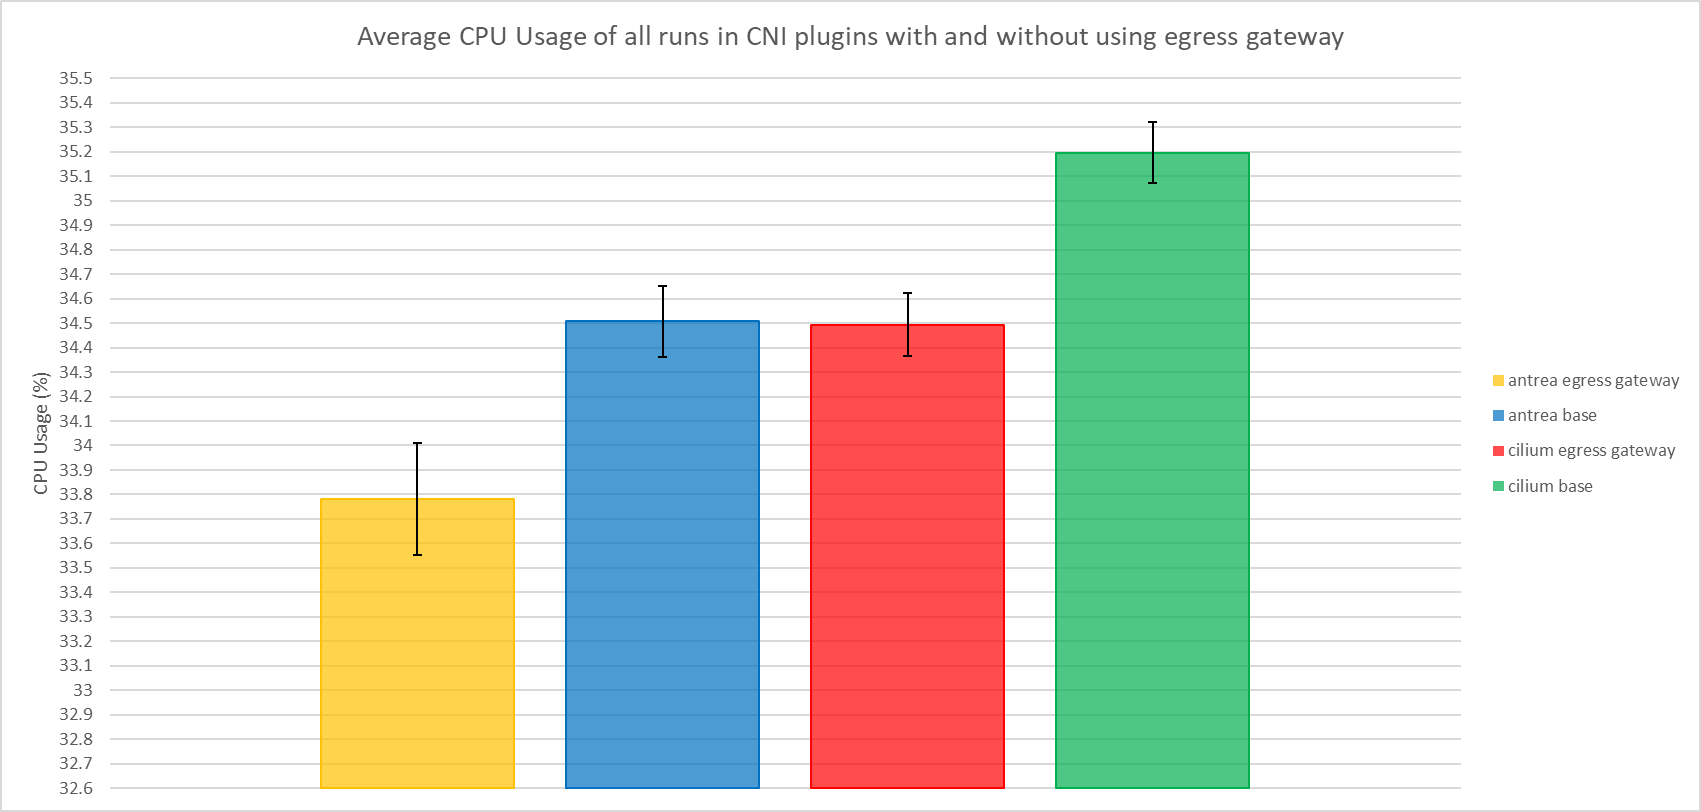
\includegraphics[width=\textwidth]{plots/egress/cpu_total_average.png}
        \caption{}
        \label{fig:cpu_avg}
    \end{subfigure}
    \begin{subfigure}[b]{0.55\textwidth}
        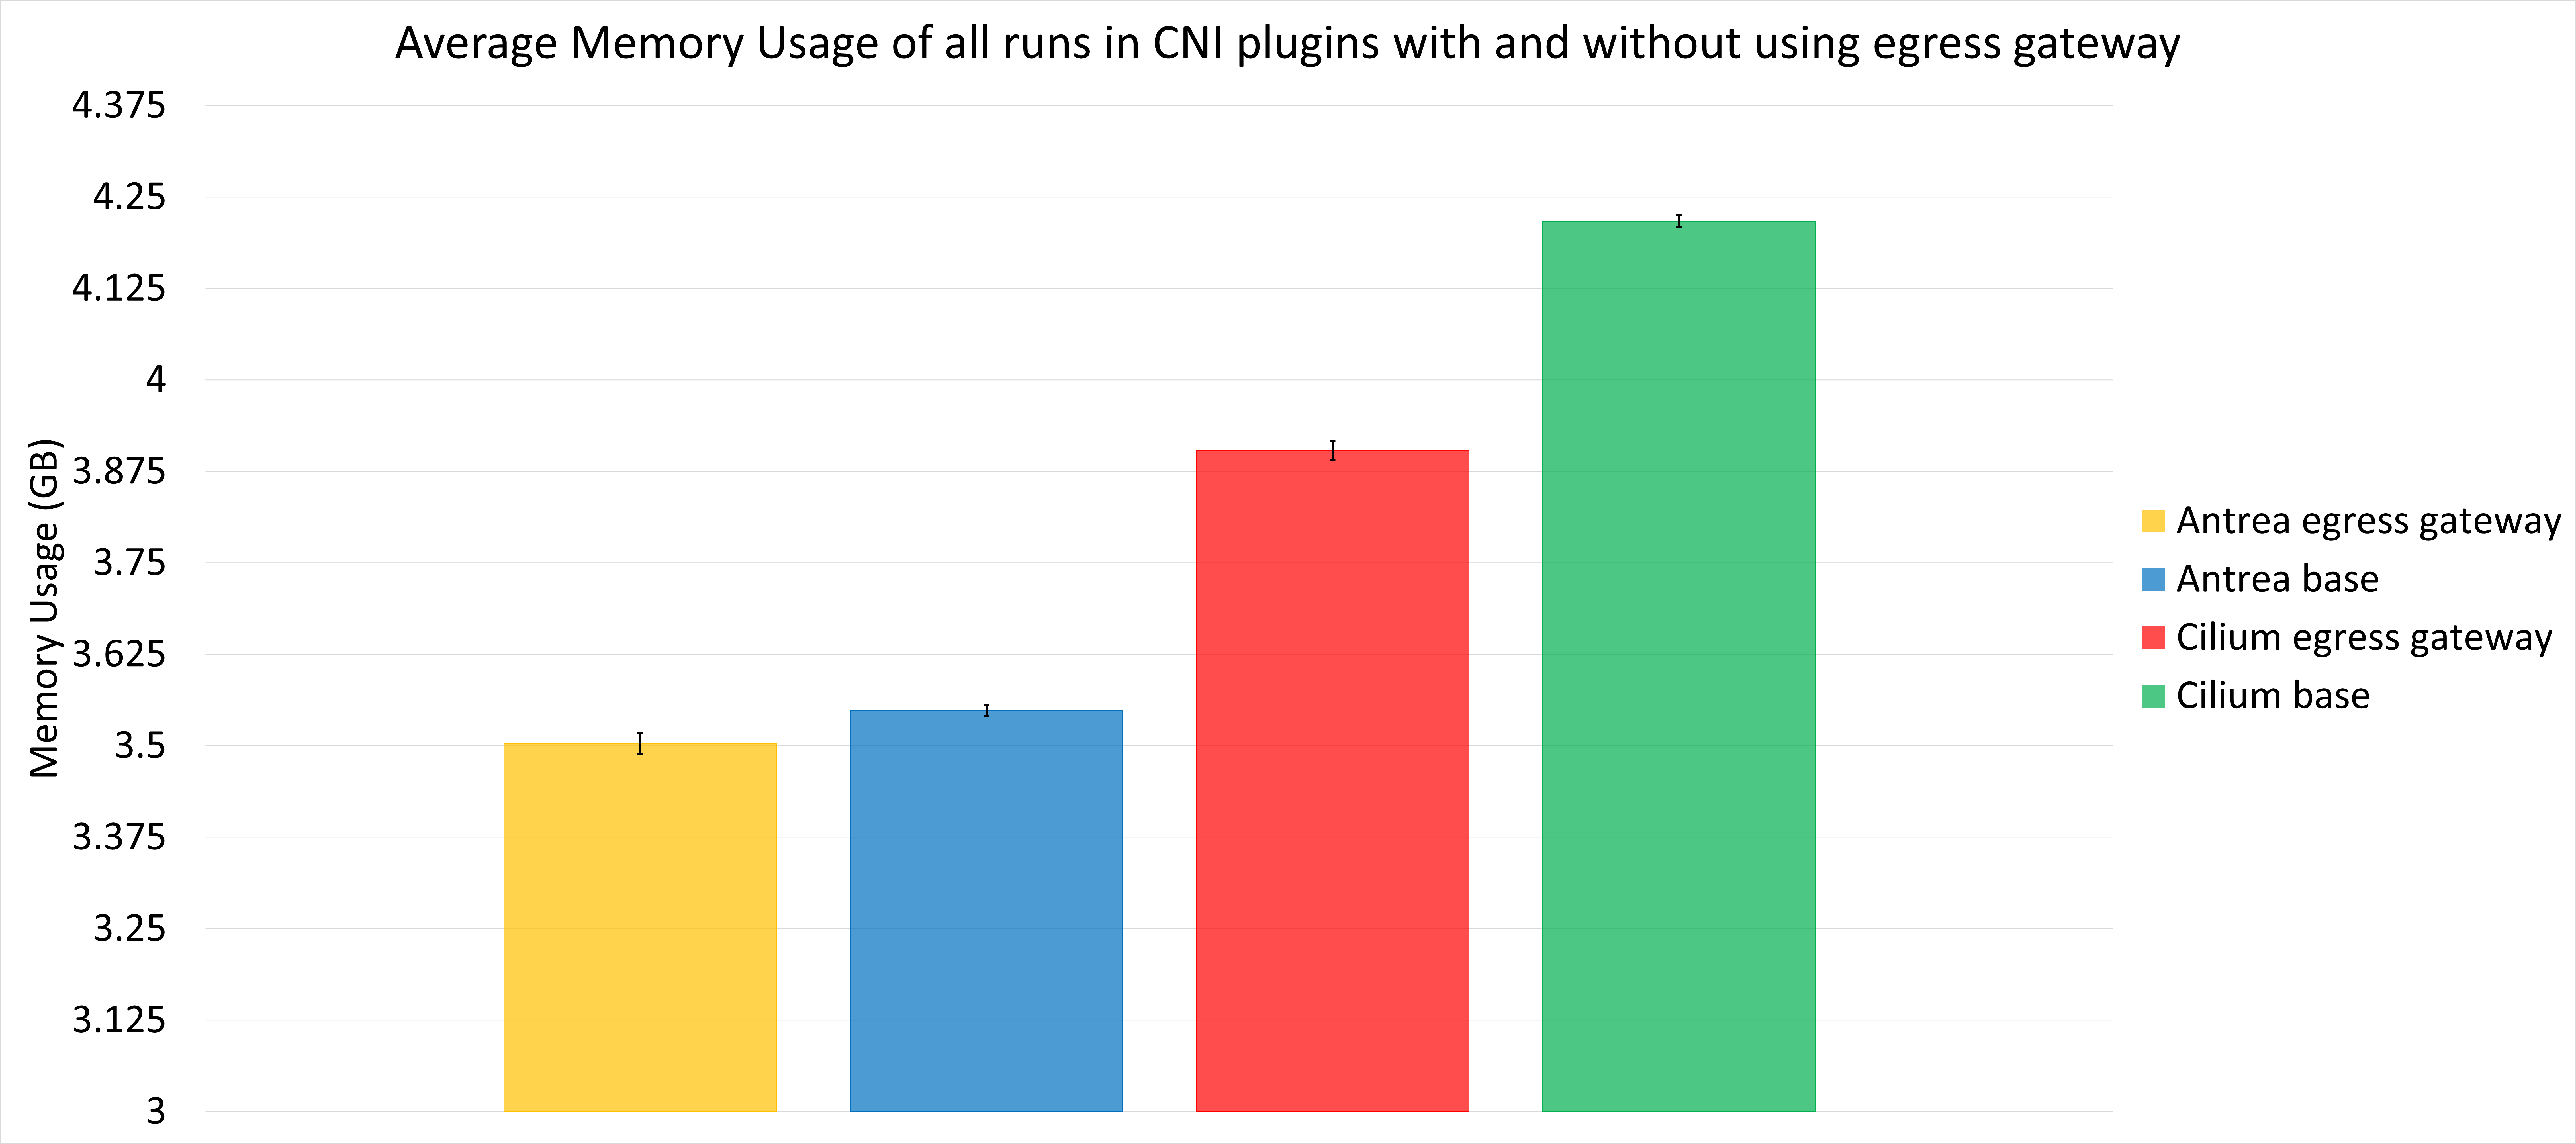
\includegraphics[width=\textwidth]{plots/egress/memory_total_average.png}
        \caption{}
        \label{fig:memory_avg}
    \end{subfigure}
    
    \caption{Average resource comsumption in egress scenario, (a) CPU, (b) Memory}
    \label{fig:res_avg}
\end{figure}


\begin{figure}[H]
    \centering
    \begin{subfigure}[b]{0.55\textwidth}
        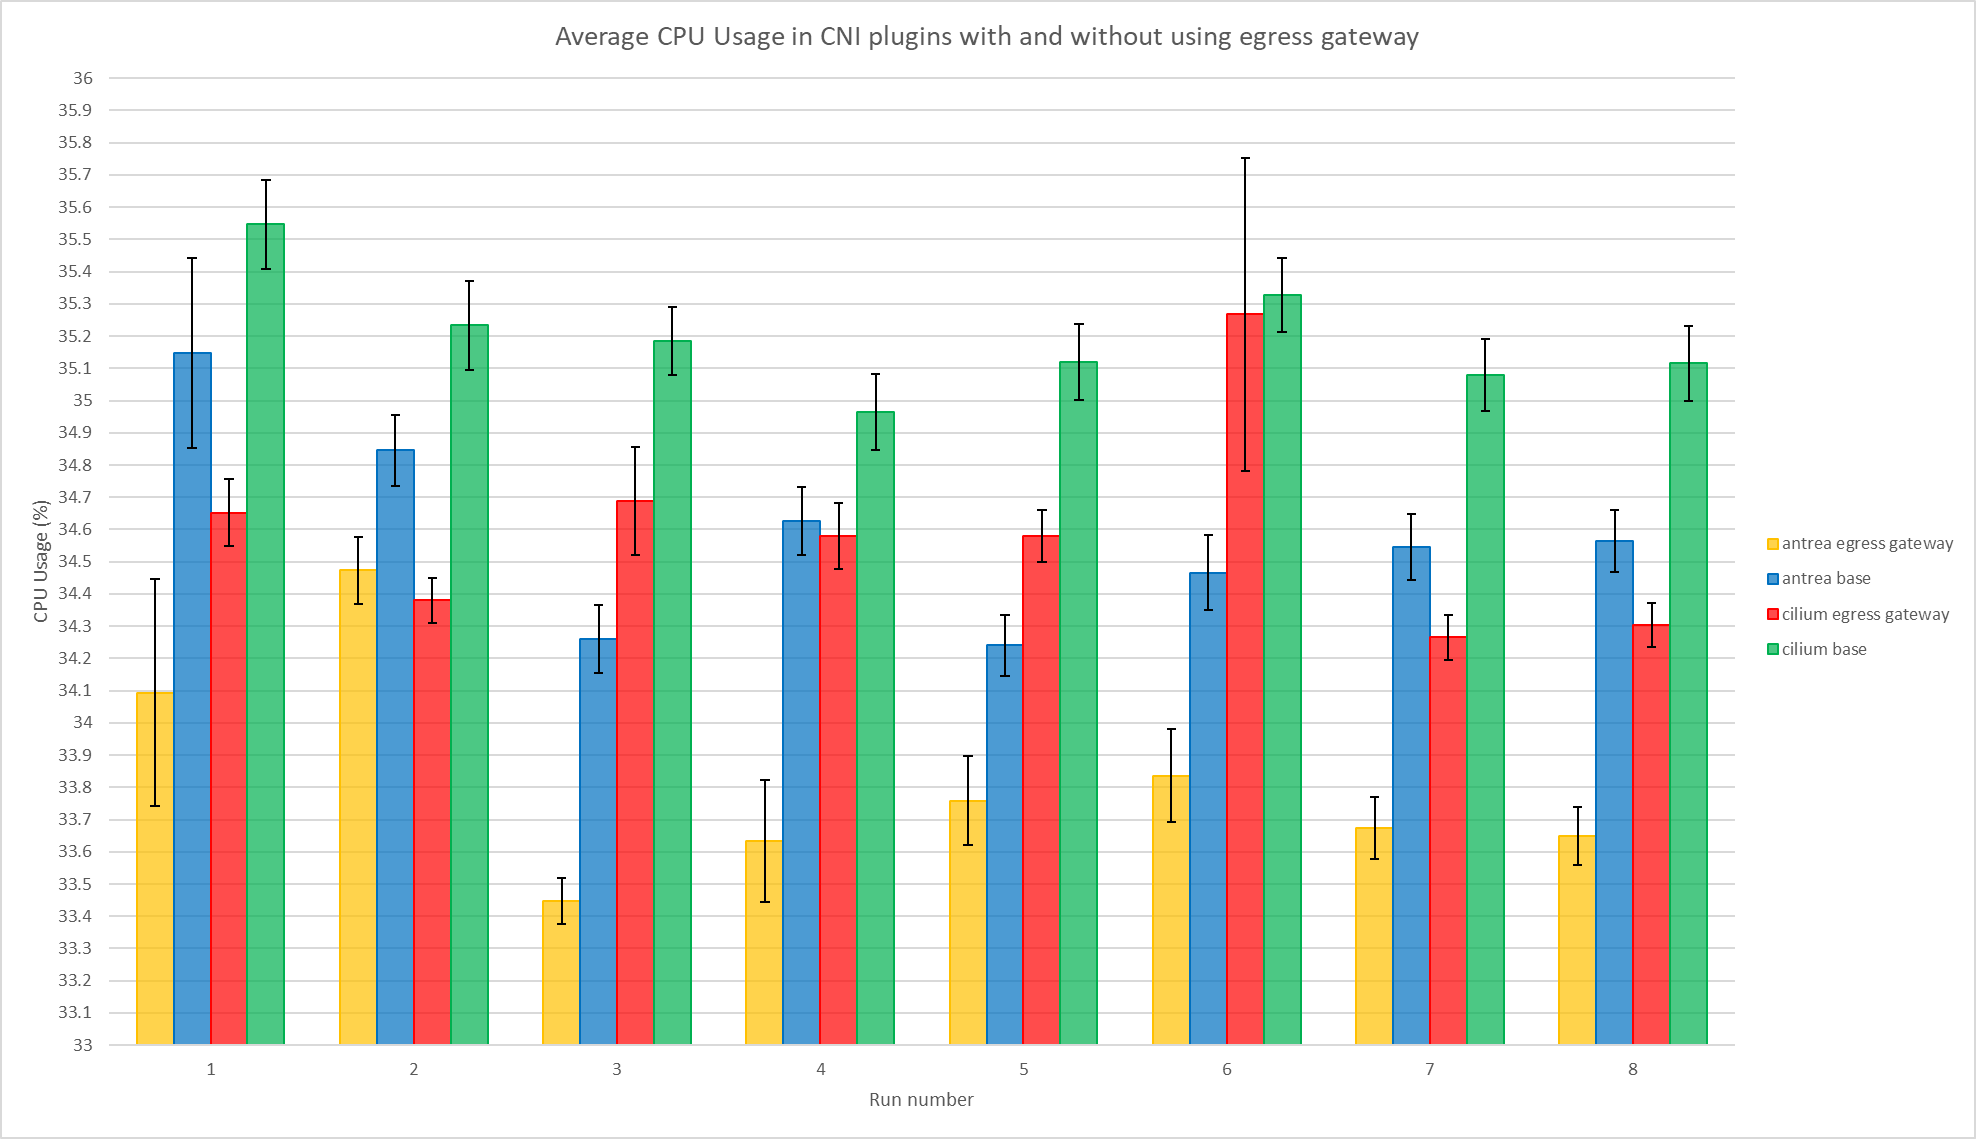
\includegraphics[width=\textwidth]{plots/egress/cpu_all.png}
        \caption{}
        \label{fig:cpu_all}
    \end{subfigure}
    \begin{subfigure}[b]{0.55\textwidth}
        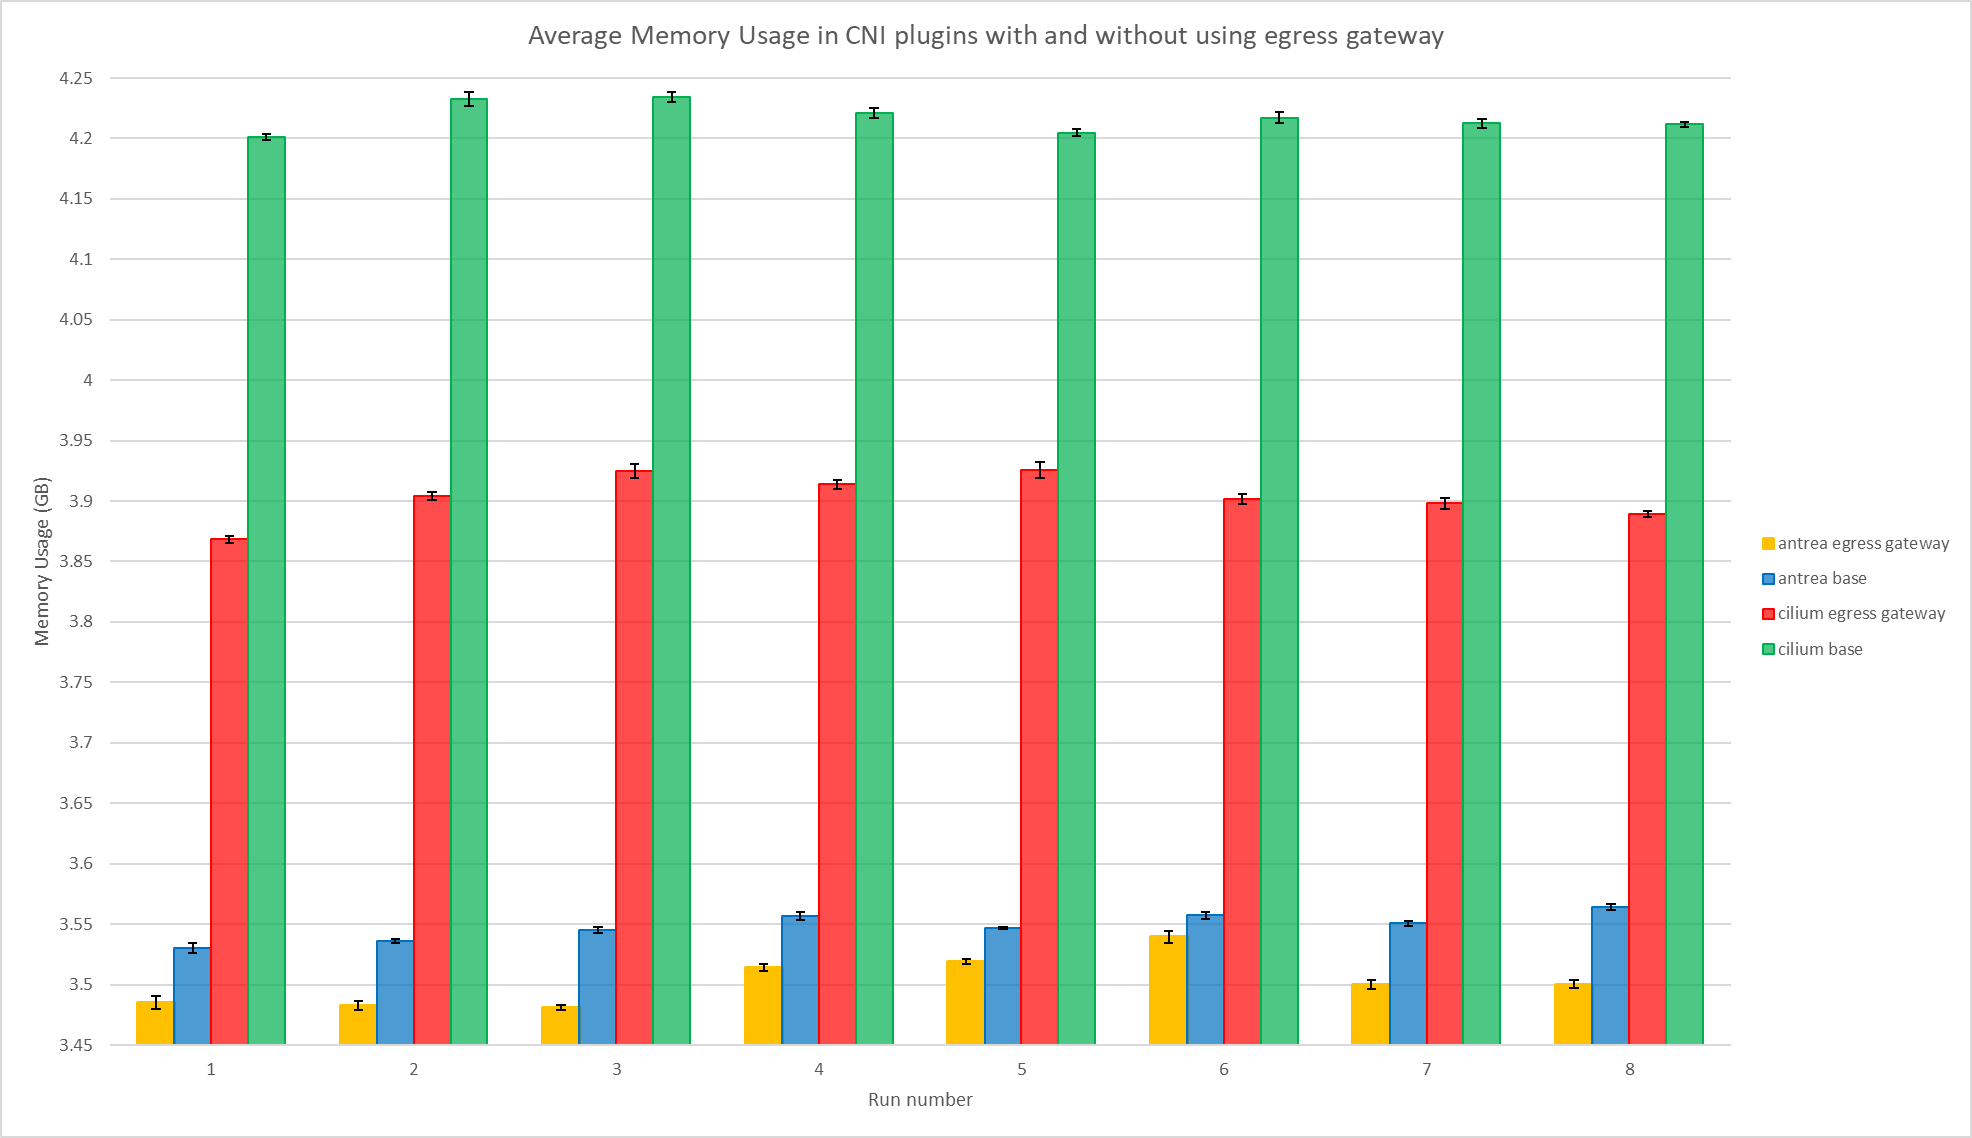
\includegraphics[width=\textwidth]{plots/egress/memory_all.png}
        \caption{}
        \label{fig:memory_all}
    \end{subfigure}
    
    \caption{Average resource comsumption in egress scenario in each run, (a) CPU, (b) Memory}
    \label{fig:res_all}
\end{figure}



\begin{figure}[H]
    \centering
    \begin{subfigure}[b]{0.35\textwidth}
        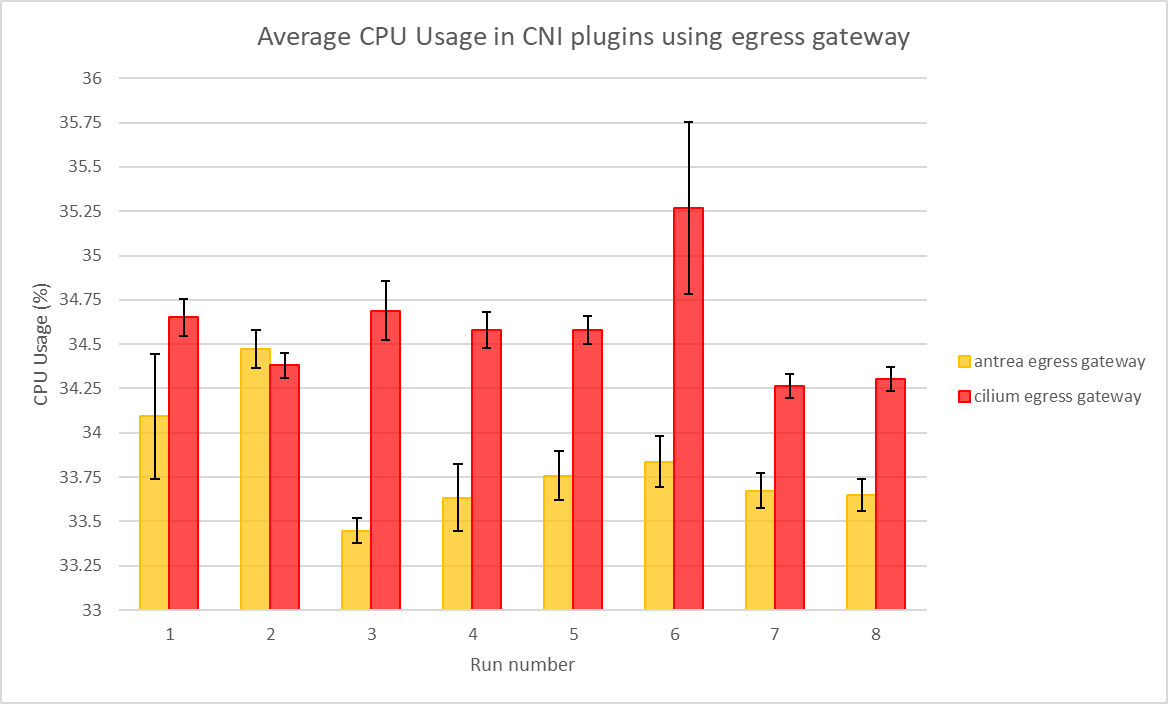
\includegraphics[width=\textwidth]{plots/small/cpu_egress.png}
        \caption{}
        \label{fig:cpu_a}
    \end{subfigure}
    \hfill
    \begin{subfigure}[b]{0.35\textwidth}
        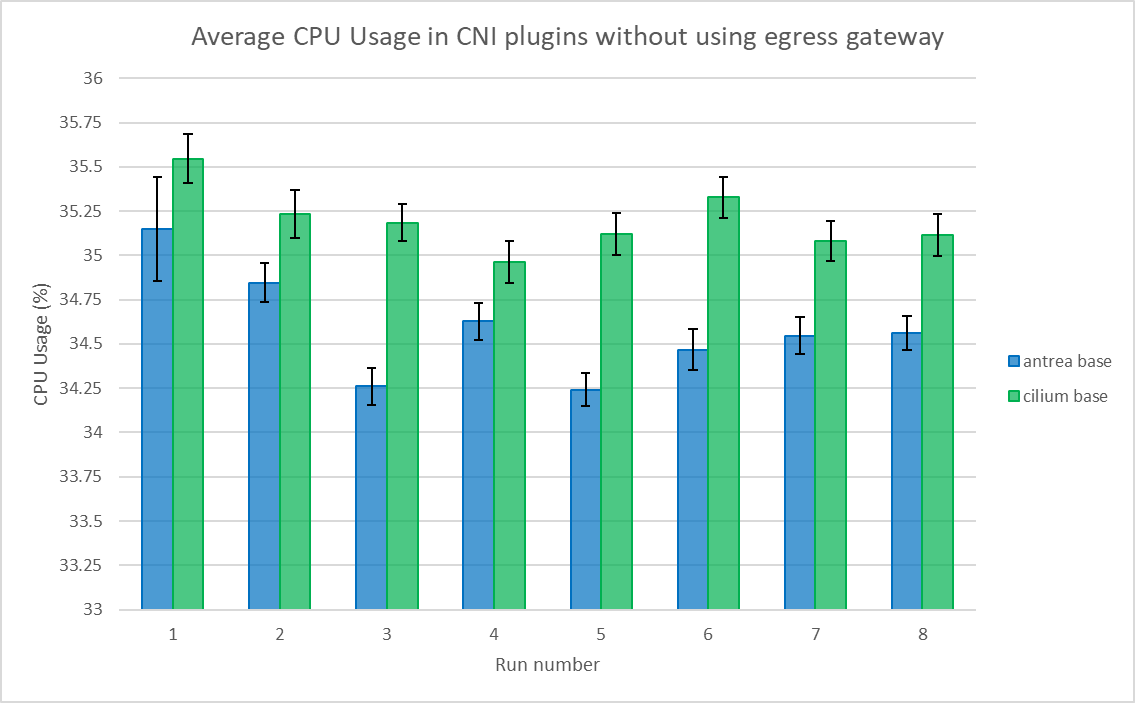
\includegraphics[width=\textwidth]{plots/small/cpu_base.png}
        \caption{}
        \label{fig:cpu_b}
    \end{subfigure}
    
    \vspace{10pt}
    
    \begin{subfigure}[b]{0.35\textwidth}
        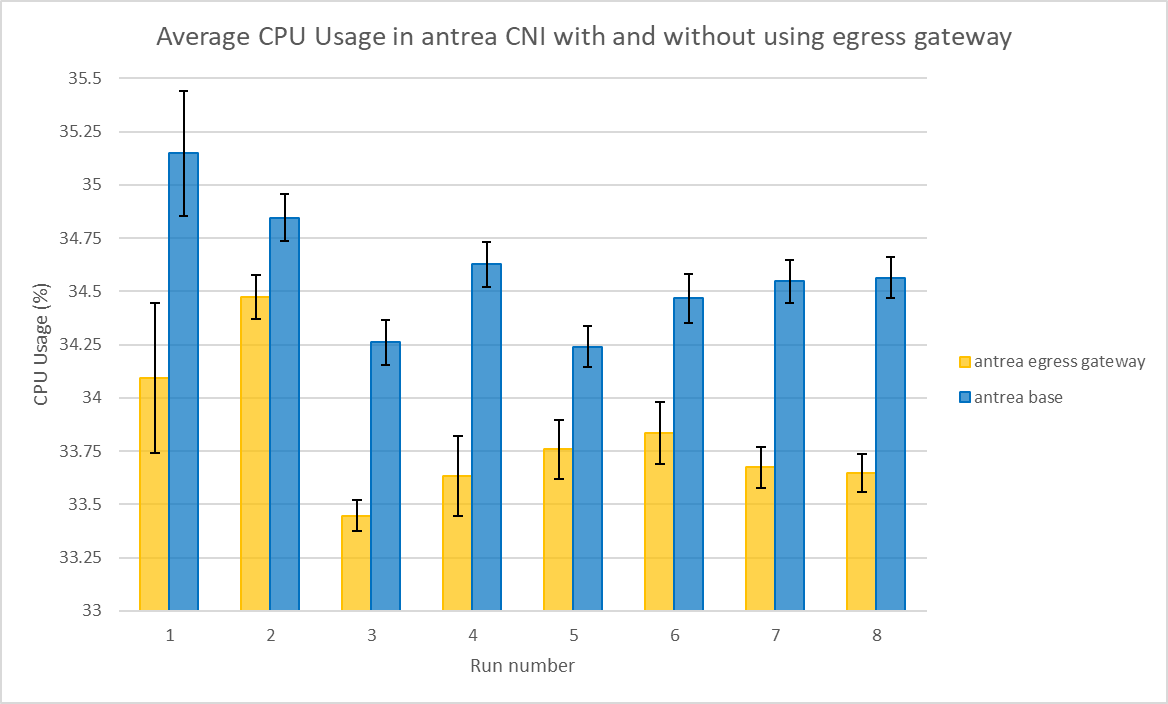
\includegraphics[width=\textwidth]{plots/small/cpu_antrea.png}
        \caption{}
        \label{fig:cpu_c}
    \end{subfigure}
    \hfill
    \begin{subfigure}[b]{0.35\textwidth}
        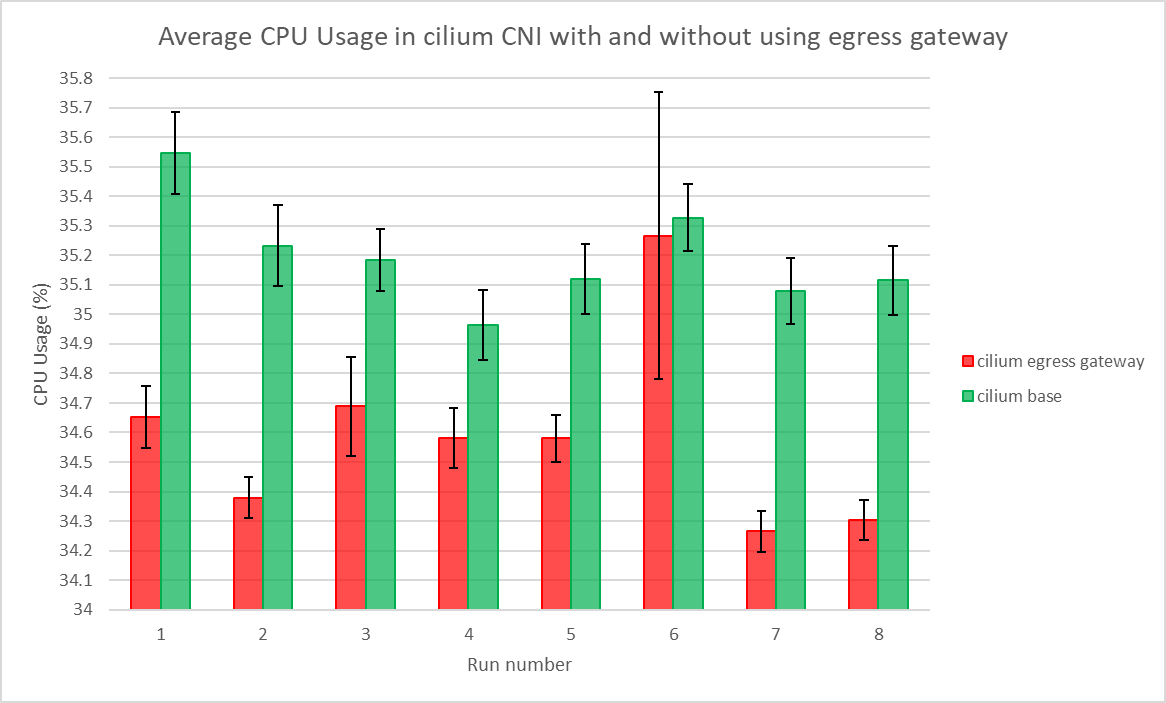
\includegraphics[width=\textwidth]{plots/small/cpu_cilium.png}
        \caption{}
        \label{fig:cpu_d}
    \end{subfigure}
    
    \caption{CPU usage in all four test cases.}
    \label{fig:cpuFour}
\end{figure}

\begin{figure}[H]
    \centering
    \begin{subfigure}[b]{0.35\textwidth}
        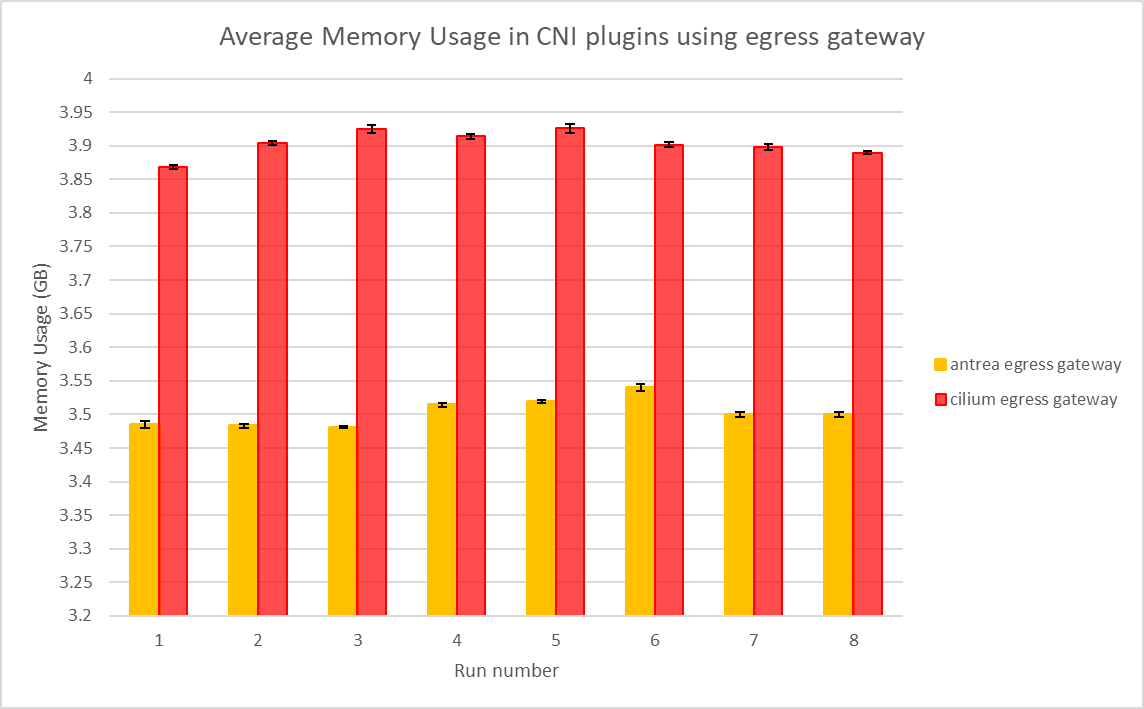
\includegraphics[width=\textwidth]{plots/small/memory_egress.png}
        \caption{}
        \label{fig:memory_a}
    \end{subfigure}
    \hfill
    \begin{subfigure}[b]{0.35\textwidth}
        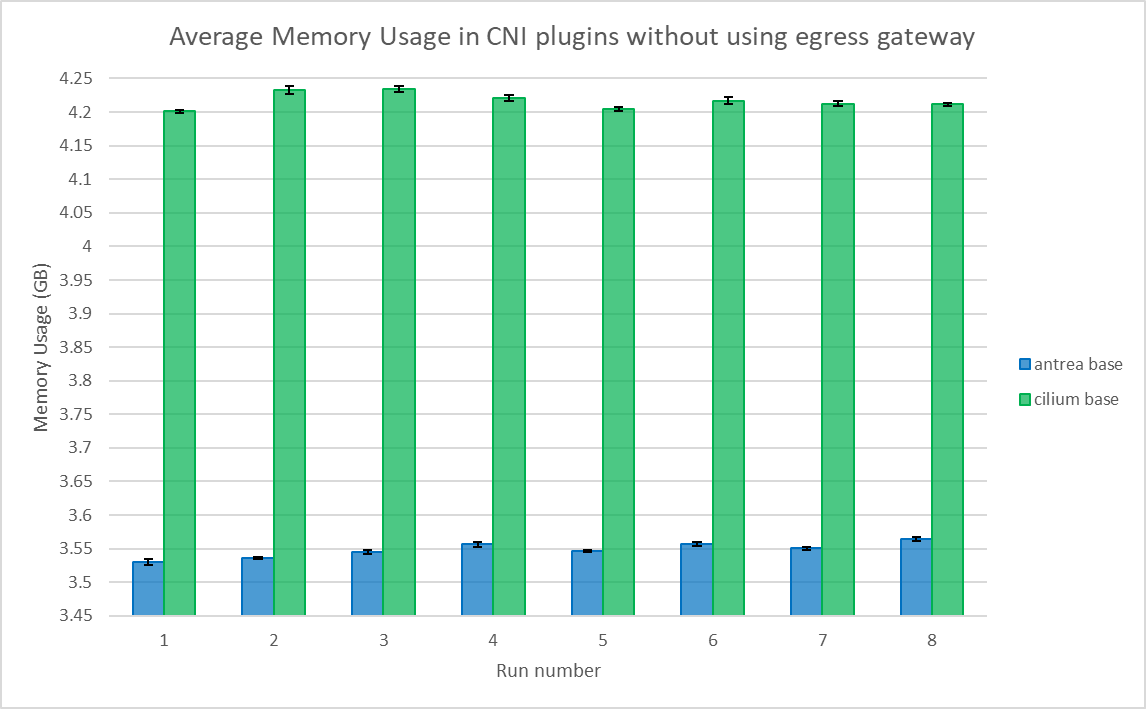
\includegraphics[width=\textwidth]{plots/small/memory_base.png}
        \caption{}
        \label{fig:memory_b}
    \end{subfigure}
    
    \vspace{10pt}
    
    \begin{subfigure}[b]{0.35\textwidth}
        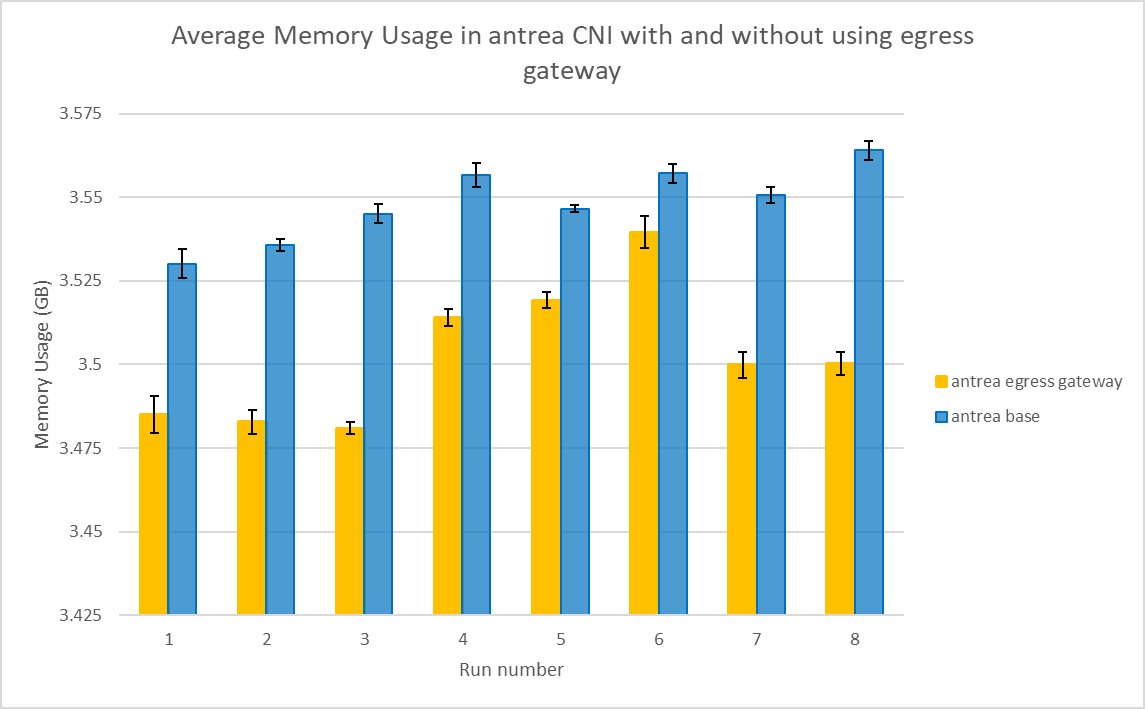
\includegraphics[width=\textwidth]{plots/small/memory_antrea.png}
        \caption{}
        \label{fig:memory_c}
    \end{subfigure}
    \hfill
    \begin{subfigure}[b]{0.35\textwidth}
        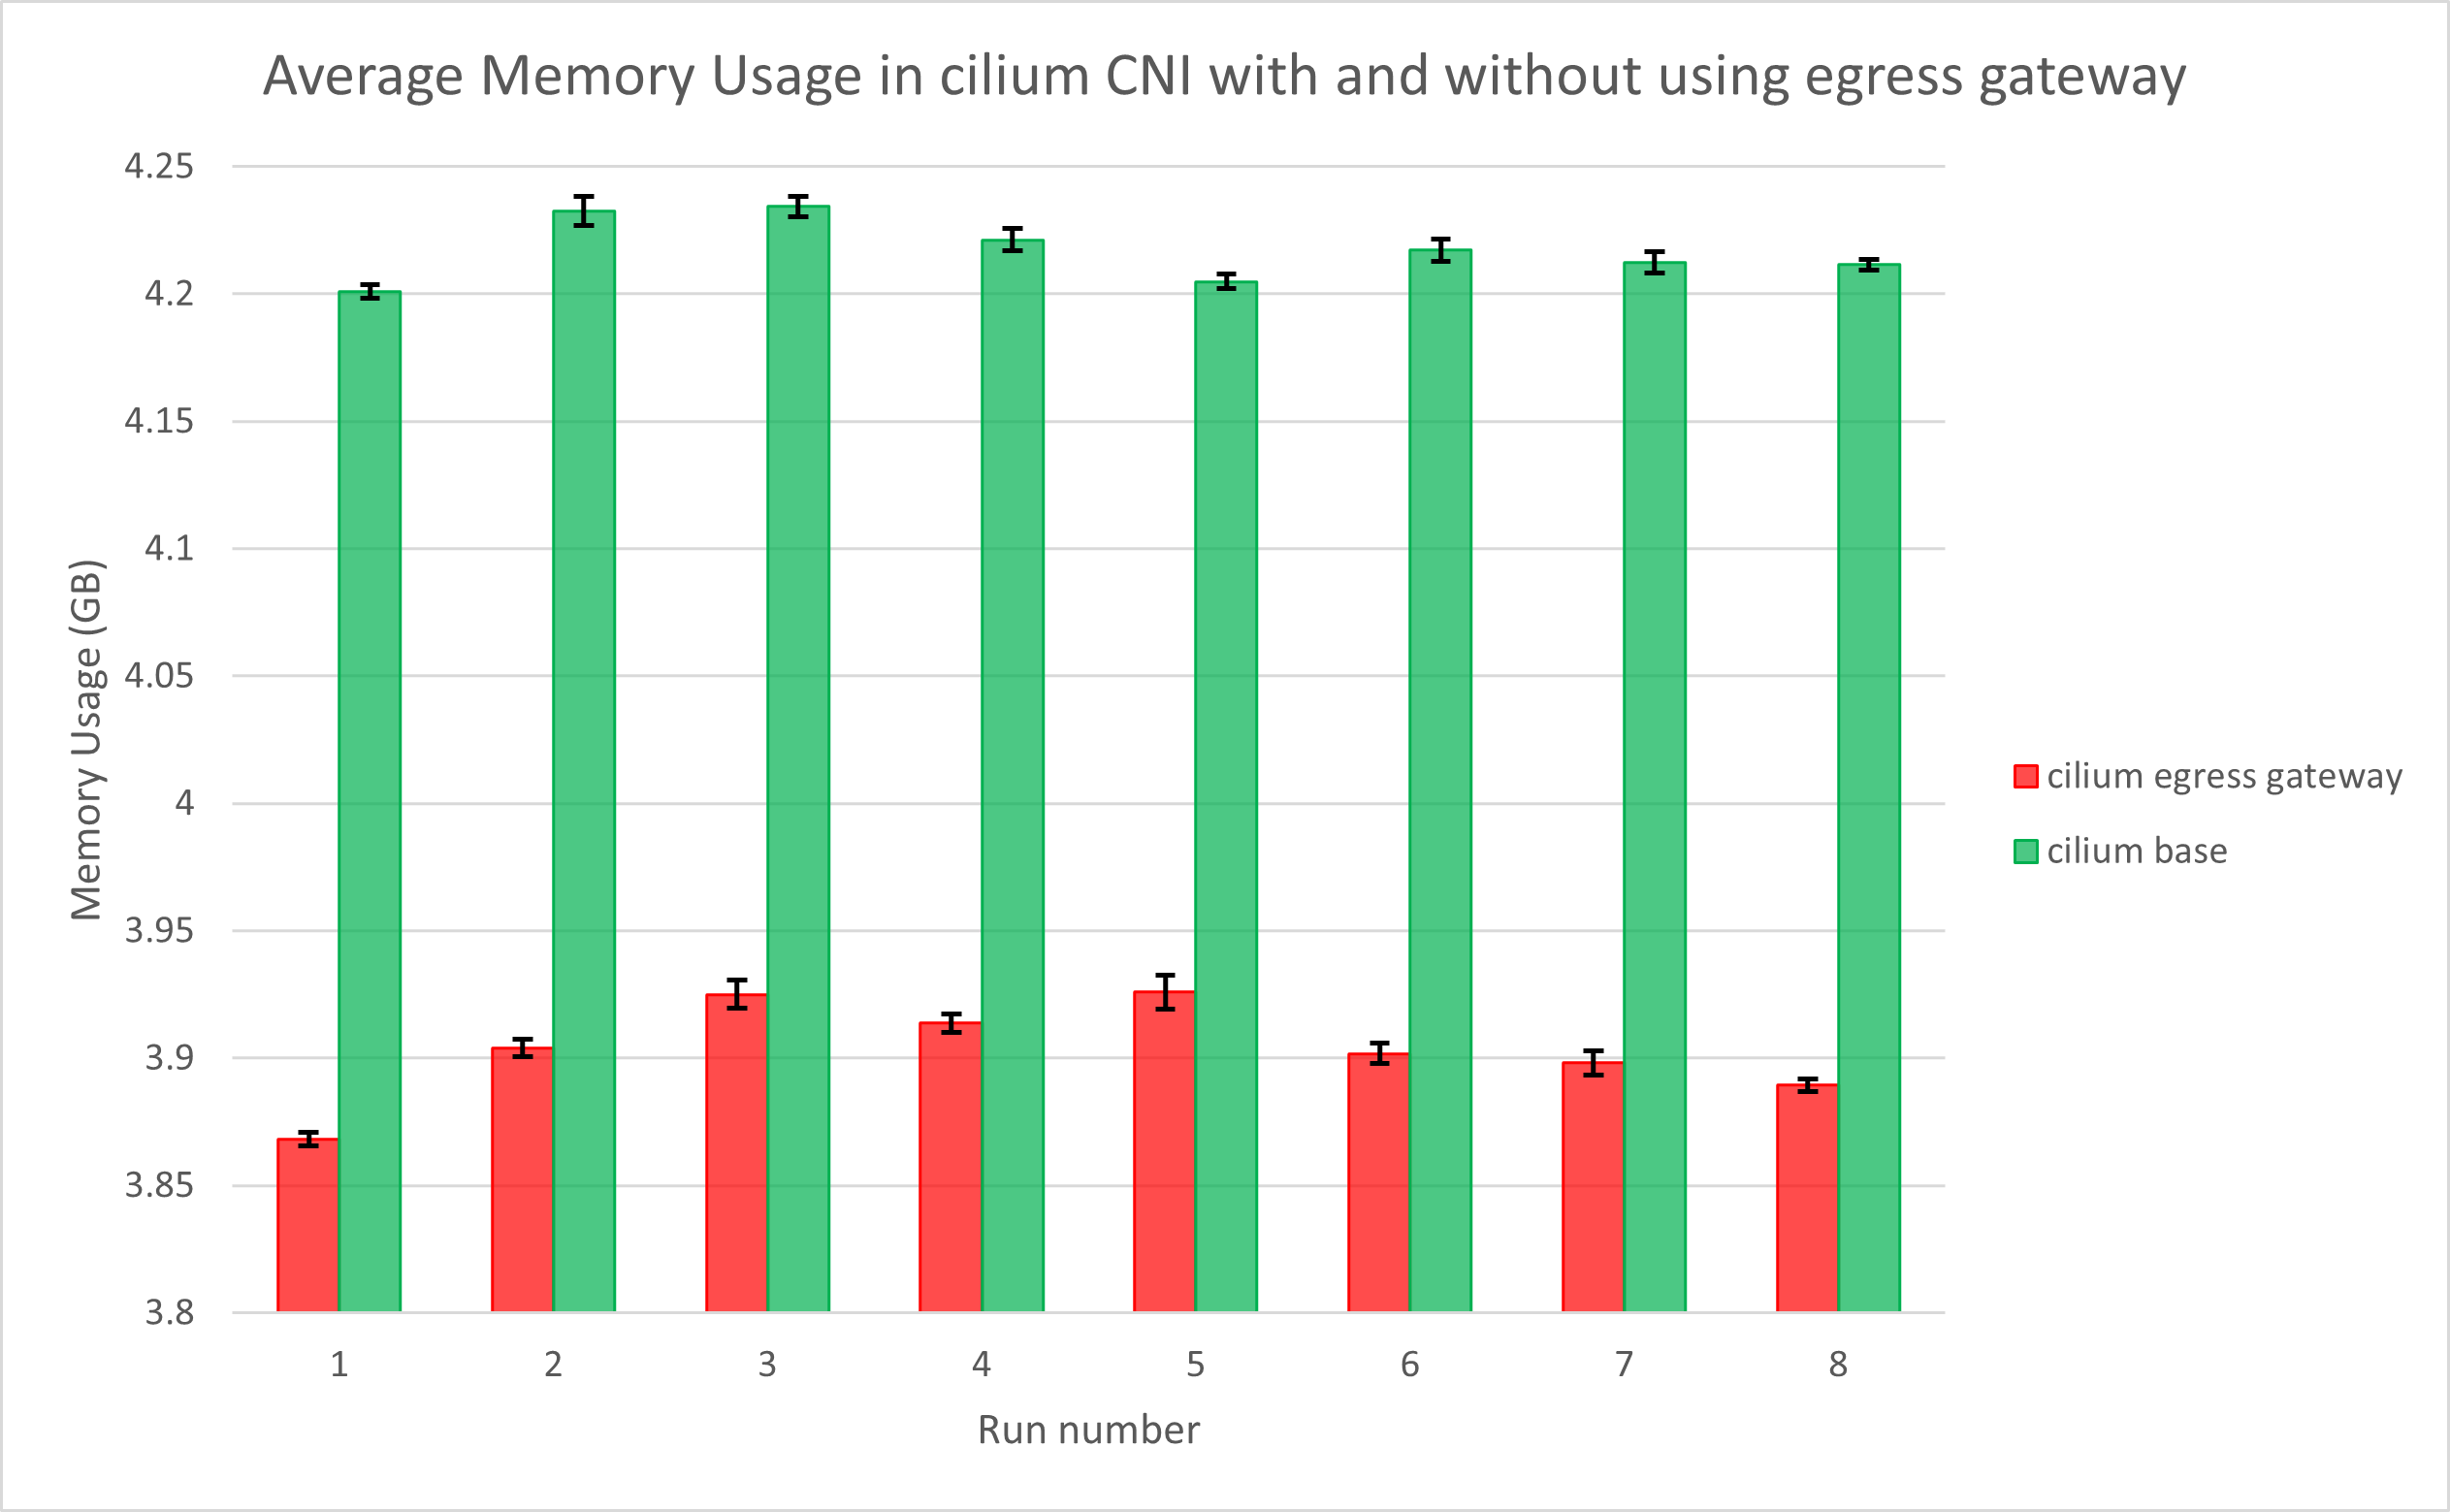
\includegraphics[width=\textwidth]{plots/small/memory_cilium.png}
        \caption{}
        \label{fig:memory_d}
    \end{subfigure}
    
    \caption{Memory usage in all four test cases.}
    \label{fig:memoryFour}
\end{figure}

Figures~\ref{fig:cpu_a},~\ref{fig:cpu_b},~\ref{fig:memory_a},~\ref{fig:memory_b} compare average CPU and memory usage between cilium and Antrea CNI in each of eight runs. It shows how both container network interface plugins perform under the same test conditions, what helps to evaluate which plugin consumes less resources. In only second run Antrea has not used less CPU than cilium used.
Comparing resource utilization showed on figures~\ref{fig:cpu_c},~\ref{fig:cpu_d},~\ref{fig:memory_c},~\ref{fig:memory_d}, highlights how using an egress gateway with each CNI plugins affects resource usage compared to not using one.

\subsubsection{Networking performance}
\label{sec:egressNetworkingPerformance}

The figures~\ref{fig:throughput_avg} and~\ref{fig:rtt_avg} provide overall performance summary as an average of all runs. Antrea handles traffic more efficiently, with lower round trip time regardless of using egress gateway or not. The plots in~\ref{fig:throughput_all} and~\ref{fig:rtt_all} display the results of all eight runs for each test case, showing that Antrea outperforms cilium in every single run, achieving higher throughput and lower bidirectional latency.

\begin{figure}[H]
    \centering
    \begin{subfigure}[b]{0.7\textwidth}
        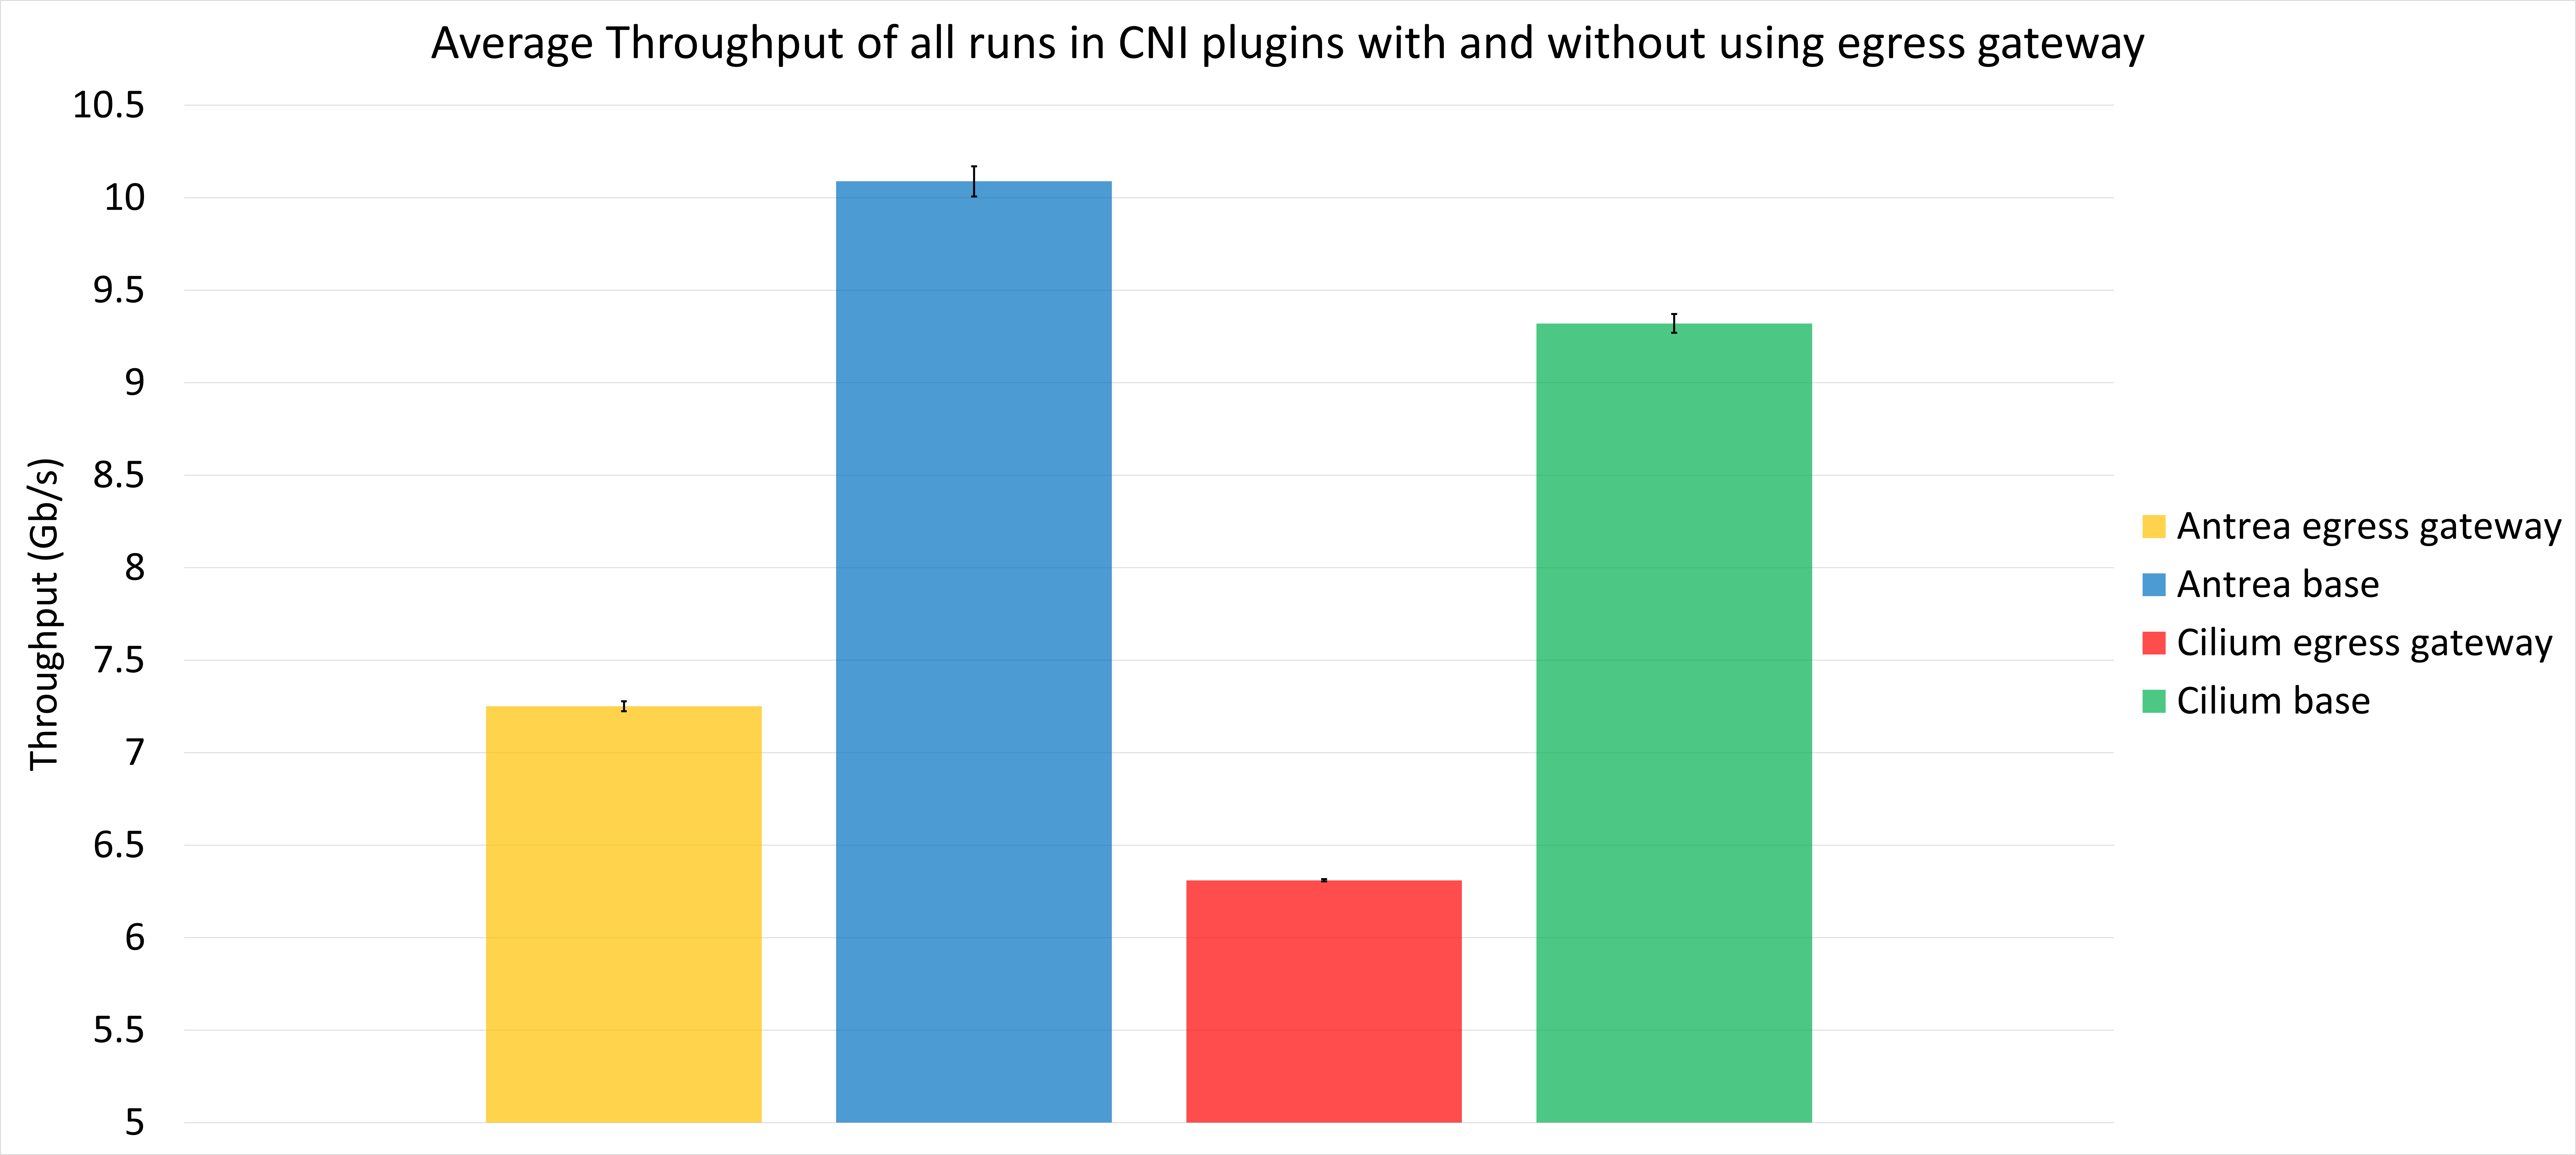
\includegraphics[width=\textwidth]{plots/egress/throughput_total_average.png}
        \caption{}
        \label{fig:throughput_avg}
    \end{subfigure}
    \begin{subfigure}[b]{0.7\textwidth}
        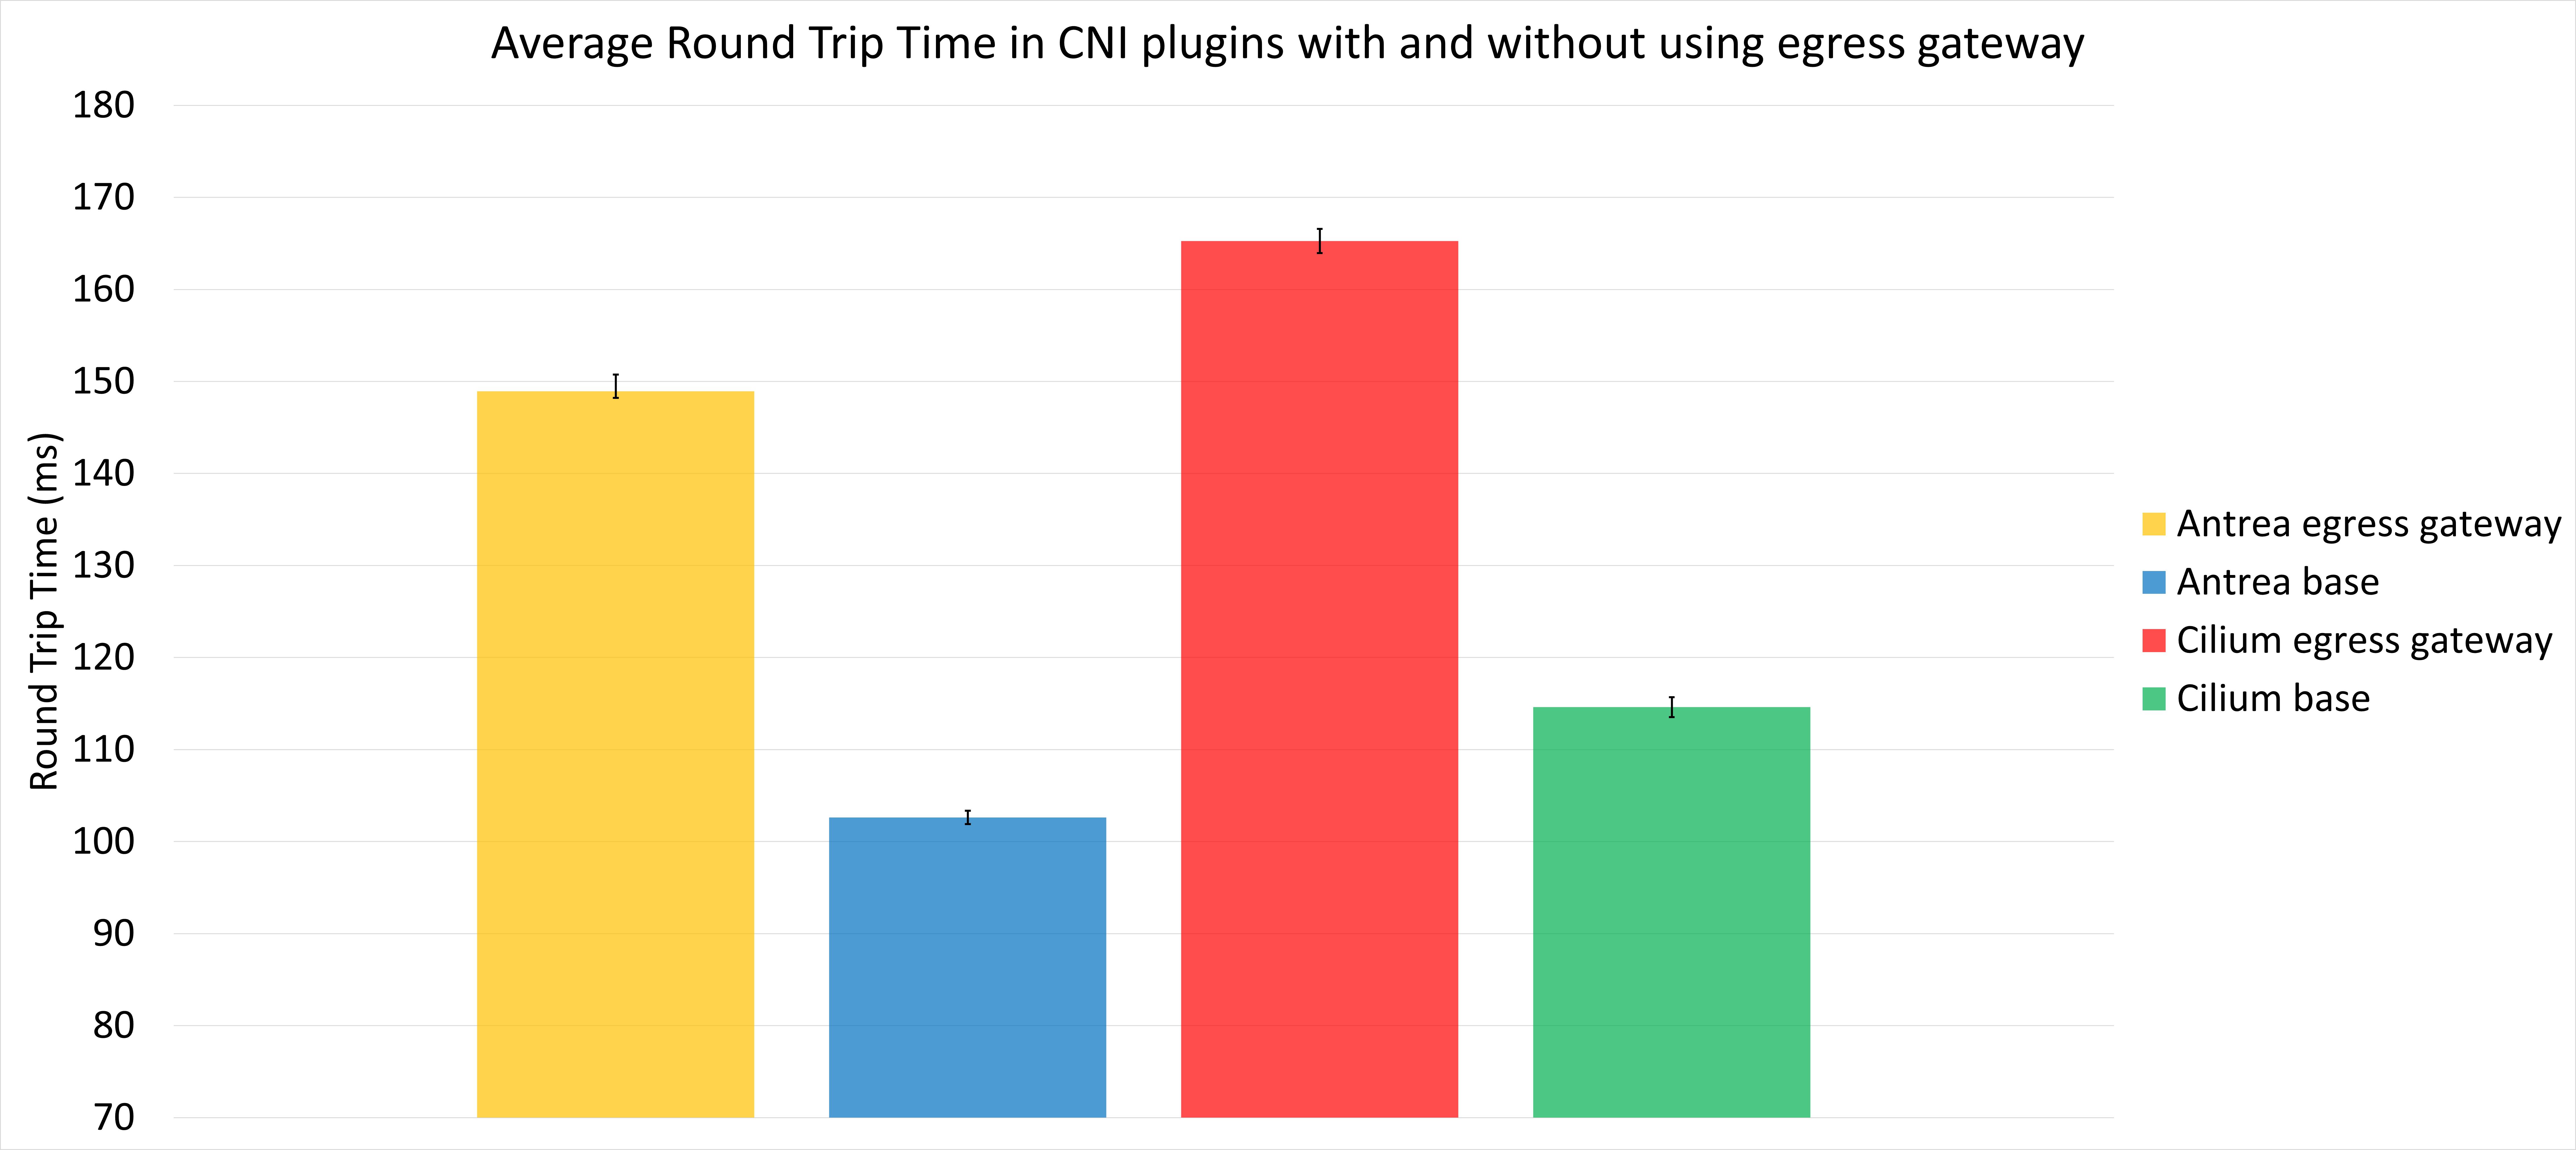
\includegraphics[width=\textwidth]{plots/egress/rtt_total_average.png}
        \caption{}
        \label{fig:rtt_avg}
    \end{subfigure}
    
    \caption{Average networking performance in egress scenario, (a) Throughput, (b) Round Trip Time}
    \label{fig:networking_avg}
\end{figure}

\begin{figure}[H]
    \centering
    \begin{subfigure}[b]{0.7\textwidth}
        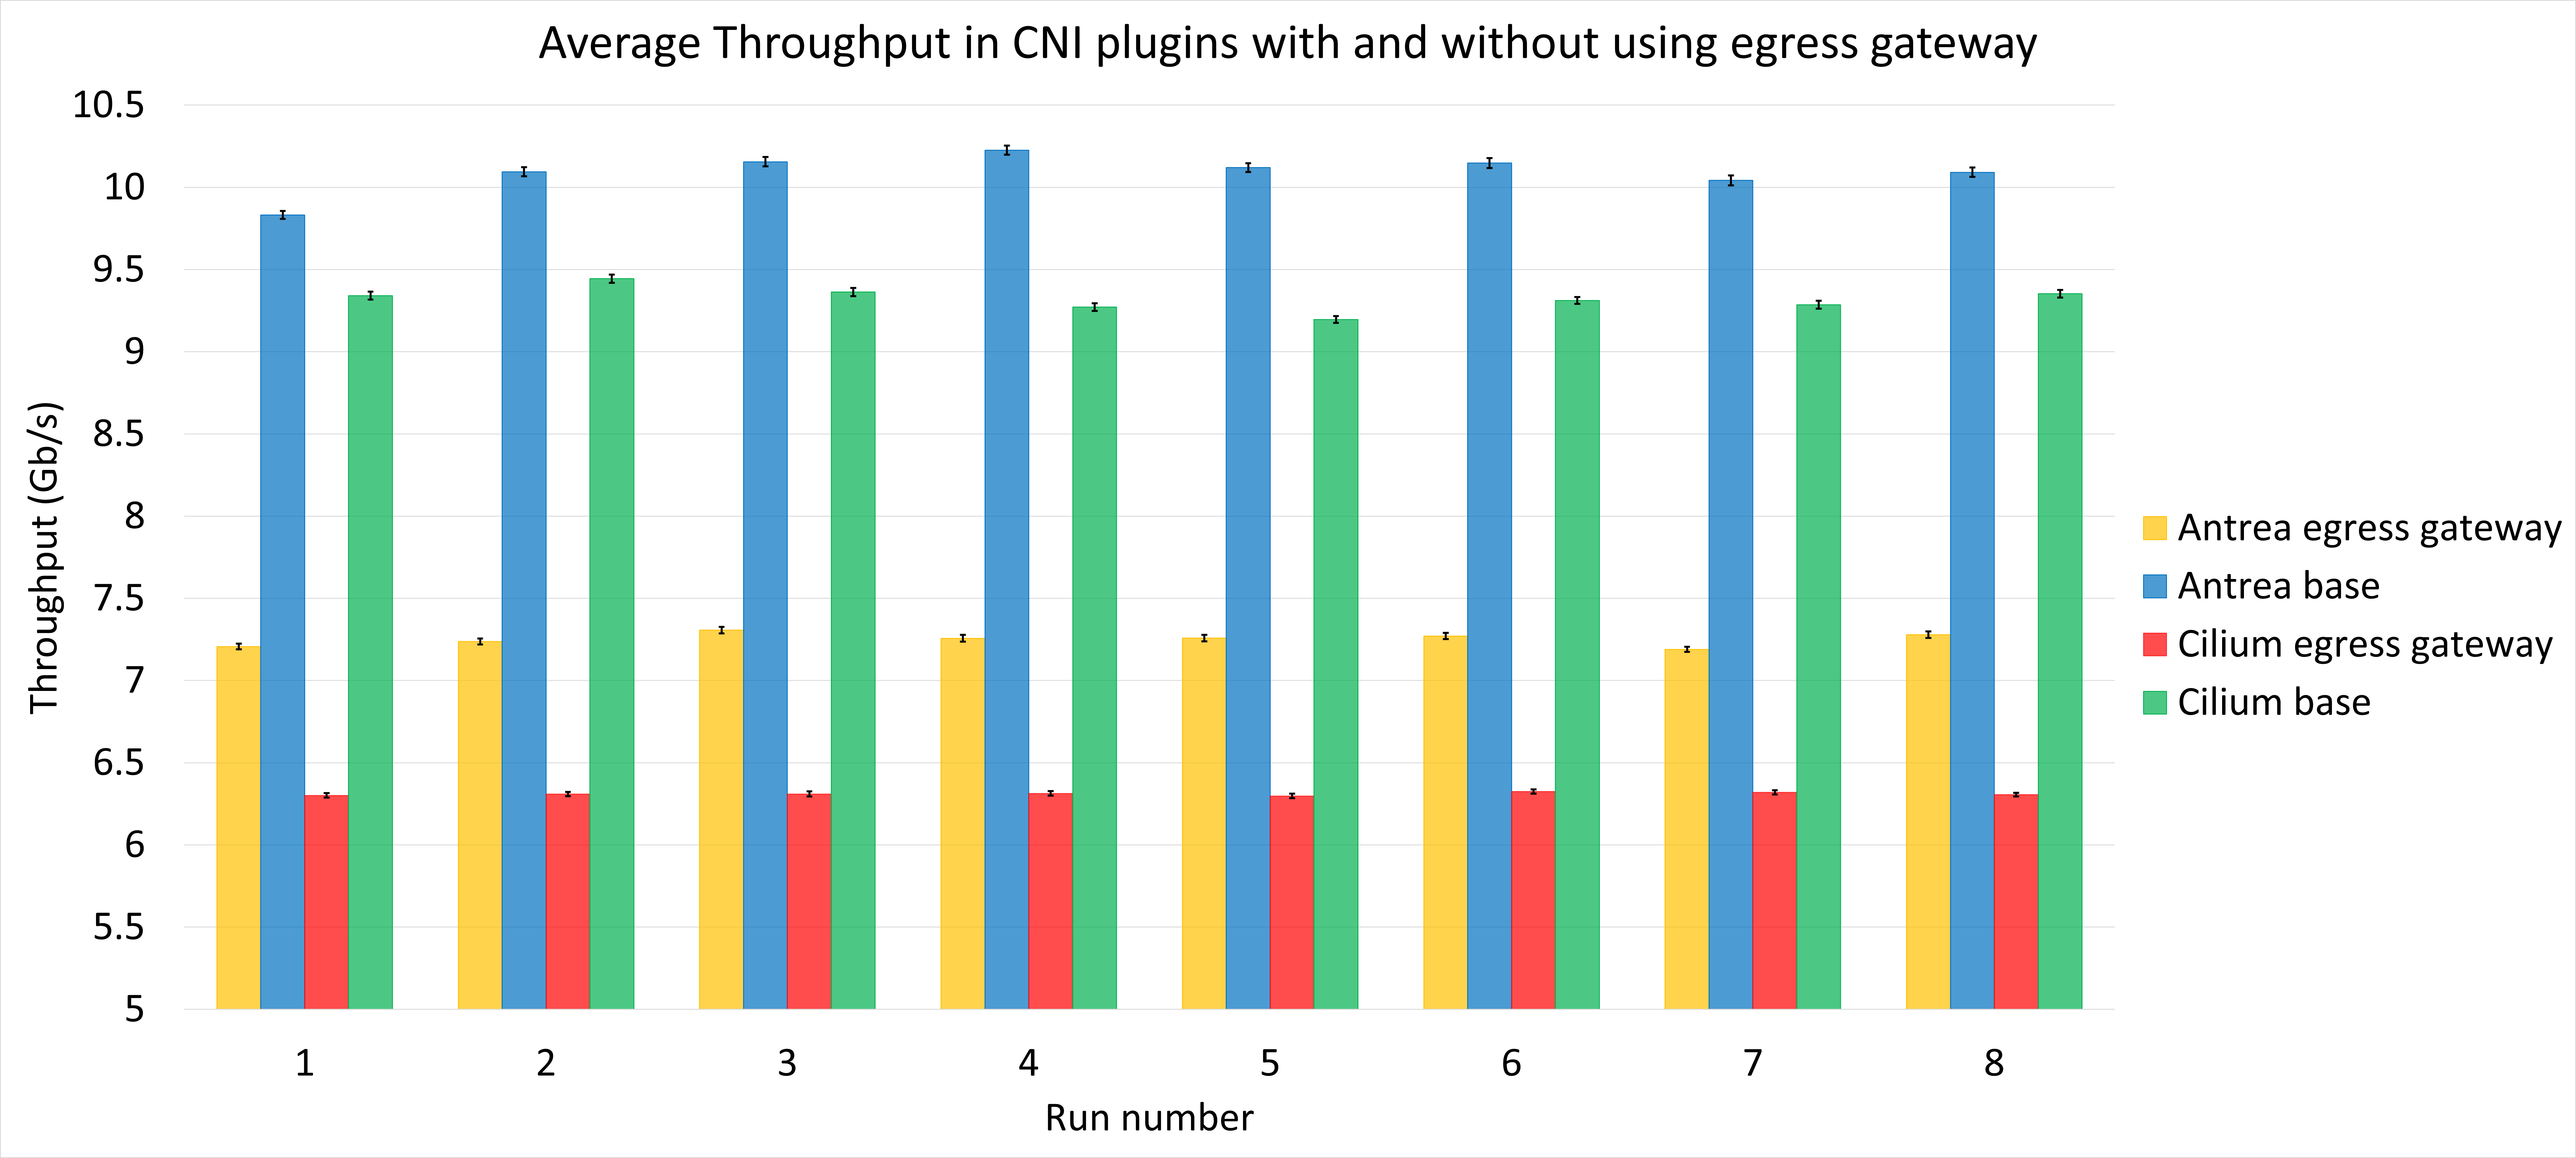
\includegraphics[width=\textwidth]{plots/egress/throughput_all.png}
        \caption{}
        \label{fig:throughput_all}
    \end{subfigure}
    \begin{subfigure}[b]{0.7\textwidth}
        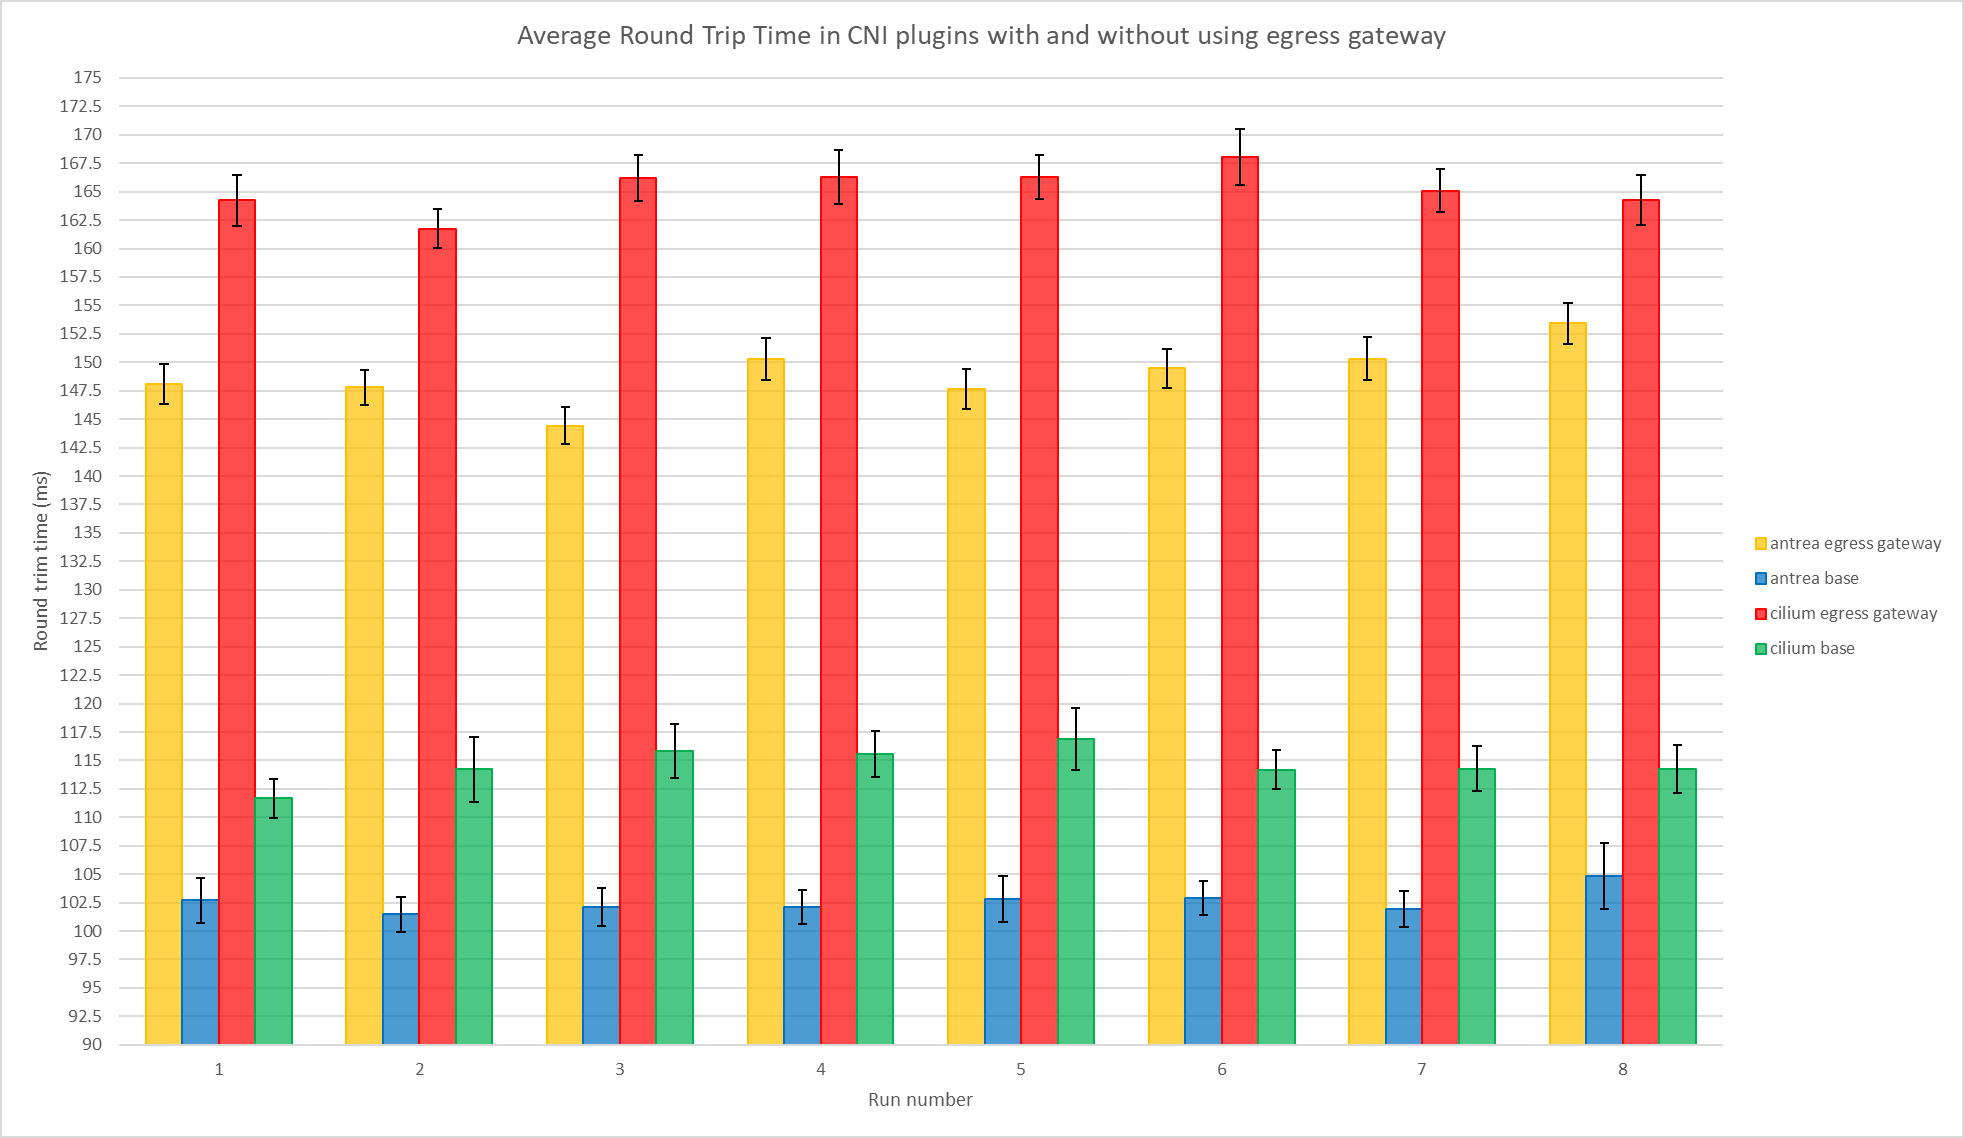
\includegraphics[width=\textwidth]{plots/egress/rtt_all.png}
        \caption{}
        \label{fig:rtt_all}
    \end{subfigure}
    
    \caption{Average networking performance in egress scenario in each run, (a) Throughput, (b) Round Trip Time}
    \label{fig:networking_avg_all}
\end{figure}




Figures~\ref{fig:throughput_a},~\ref{fig:throughput_b},~\ref{fig:rtt_a},~\ref{fig:rtt_b} illustrate average throughput and round trip time in eight runs, comparing the performance of networking plugins. Throughput with cilium egress gateway remains stable, hovering around 6.3 Gb/s and with tighter confidence intervals indicating more stability. Every single run shows the Antrea's advantage in transfer data rate and RTT.
Figures~\ref{fig:throughput_c},~\ref{fig:throughput_d},~\ref{fig:rtt_c}, and~\ref{fig:rtt_d} compare the performance of CNI plugins with and without the use of an egress gateway. They highlight whether using an egress gateway is worth, showing significant differences in throughput and round-trip time.


\begin{figure}[H]
    \centering
    \begin{subfigure}[b]{0.45\textwidth}
        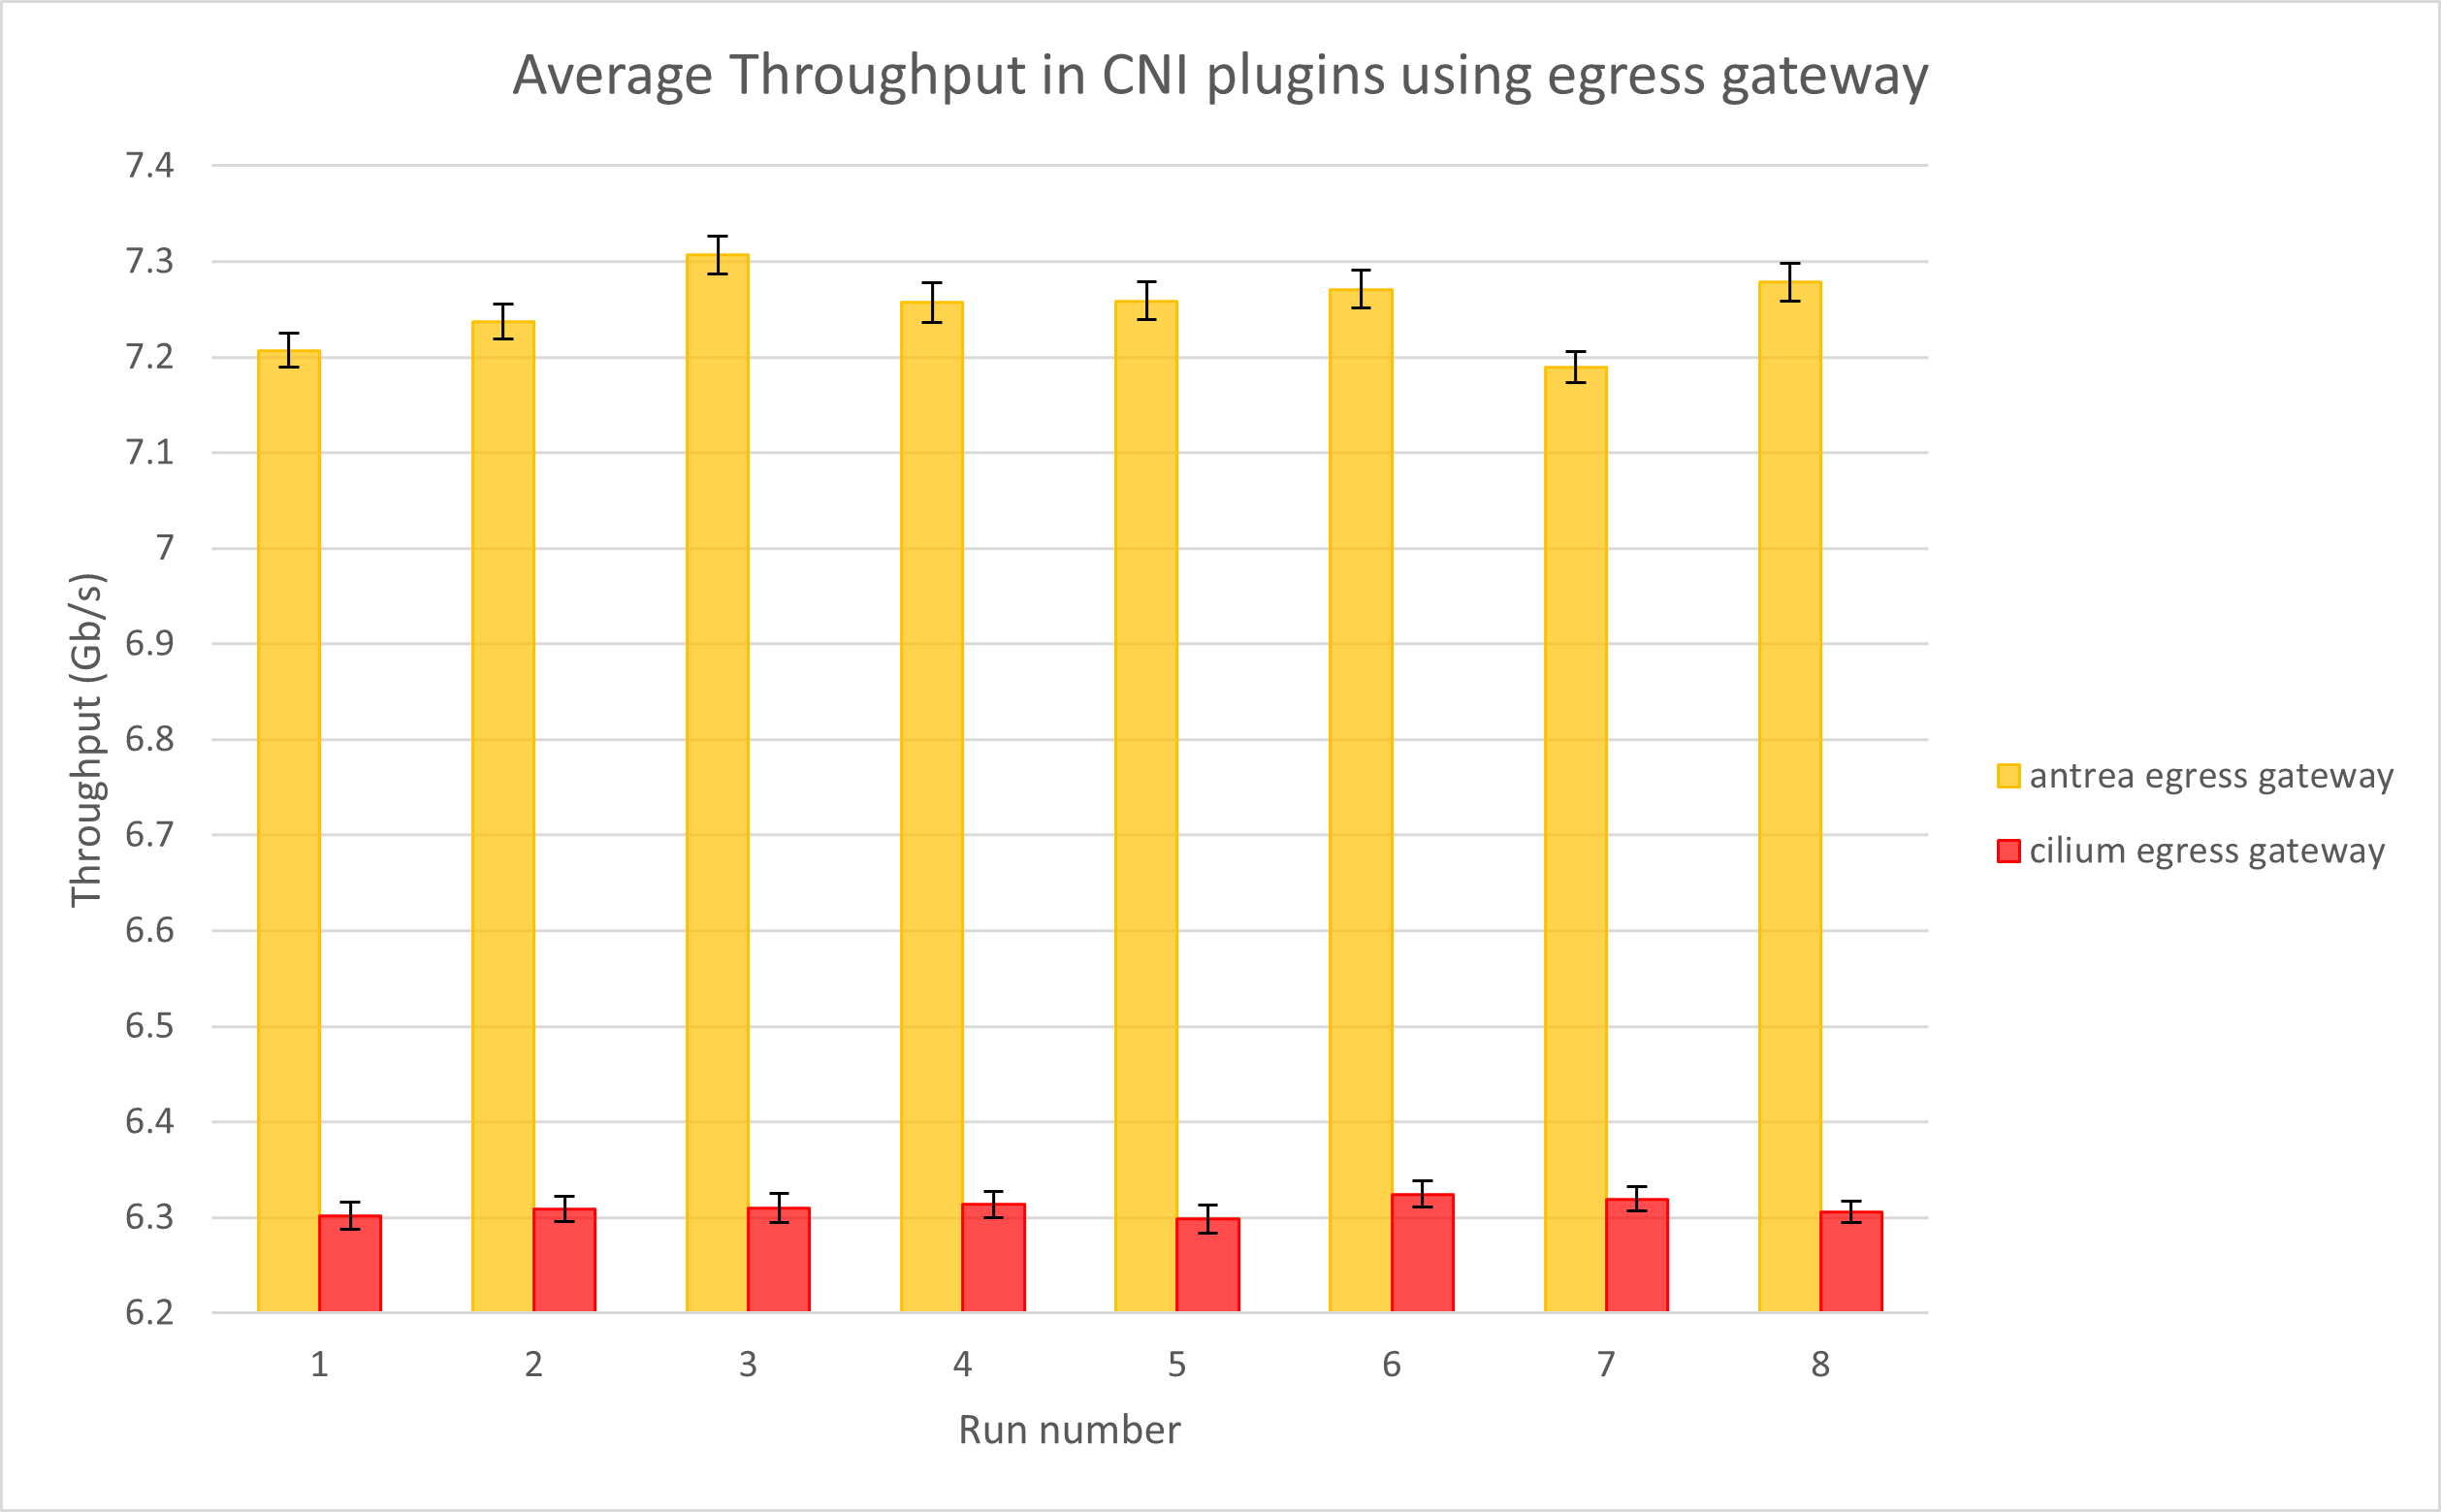
\includegraphics[width=\textwidth]{plots/small/throughput_egress.png}
        \caption{}
        \label{fig:throughput_a}
    \end{subfigure}
    \hfill
    \begin{subfigure}[b]{0.45\textwidth}
        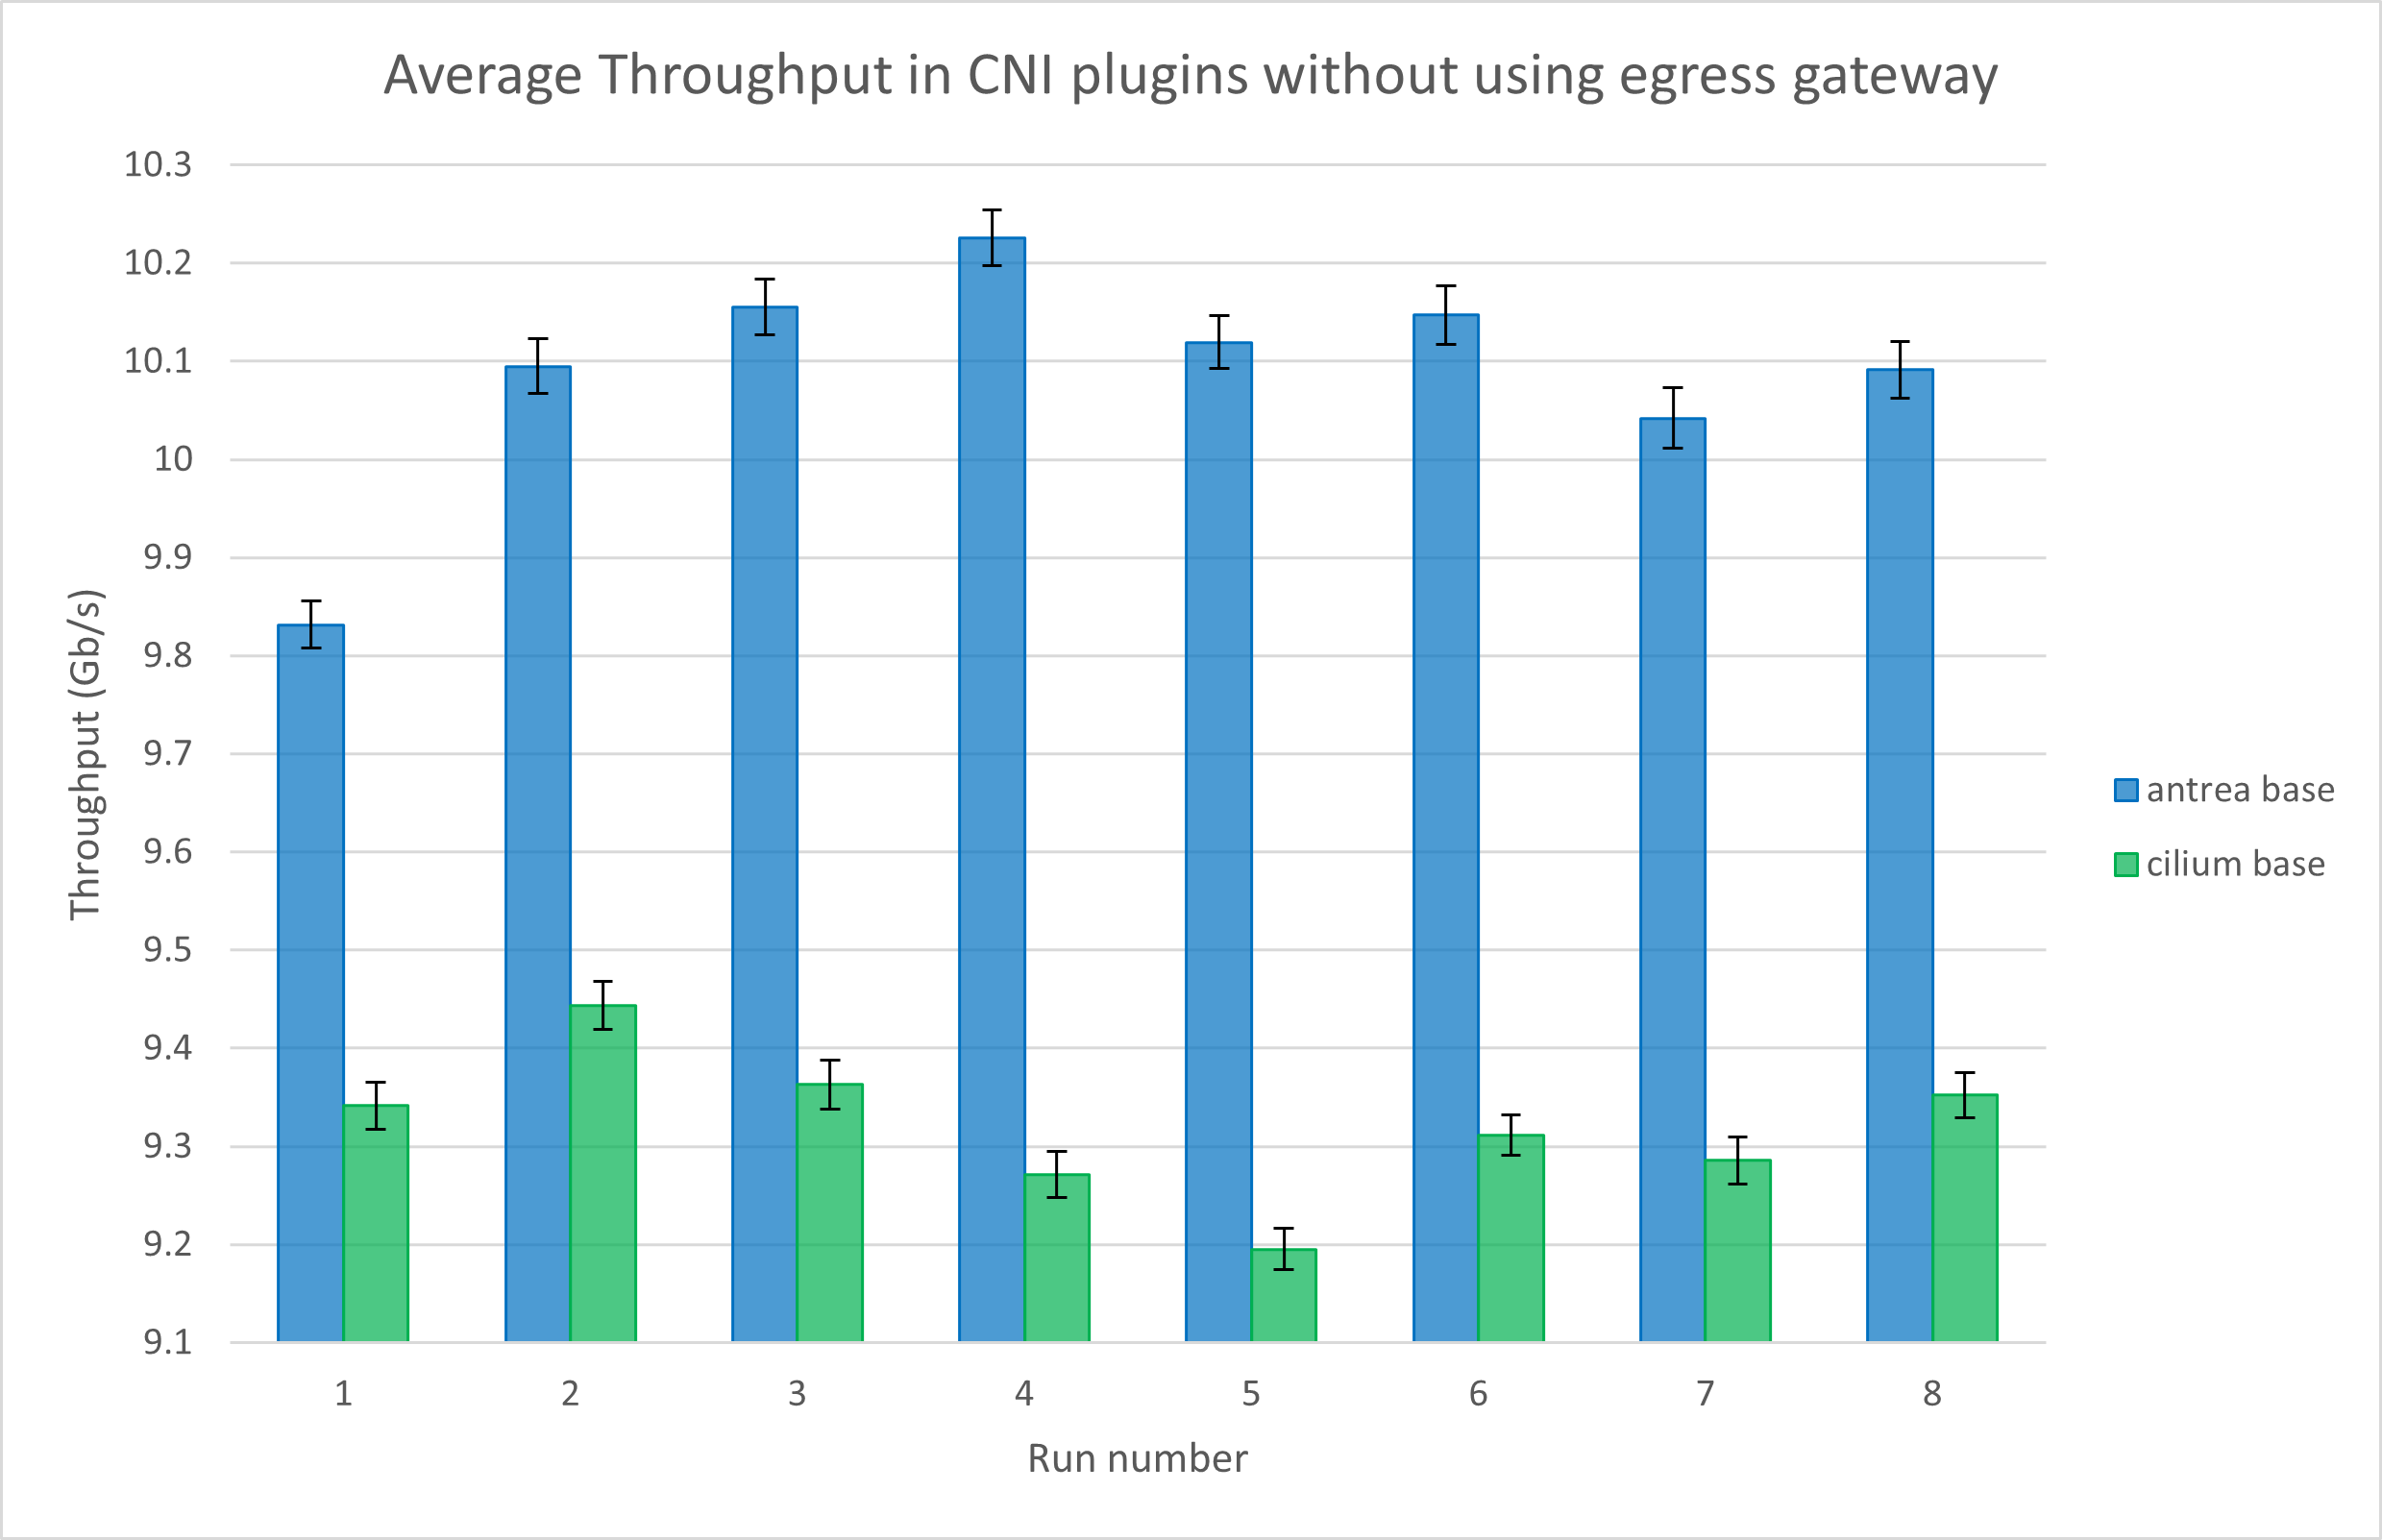
\includegraphics[width=\textwidth]{plots/small/throughput_base.png}
        \caption{}
        \label{fig:throughput_b}
    \end{subfigure}
    
    \vspace{10pt}
    
    \begin{subfigure}[b]{0.45\textwidth}
        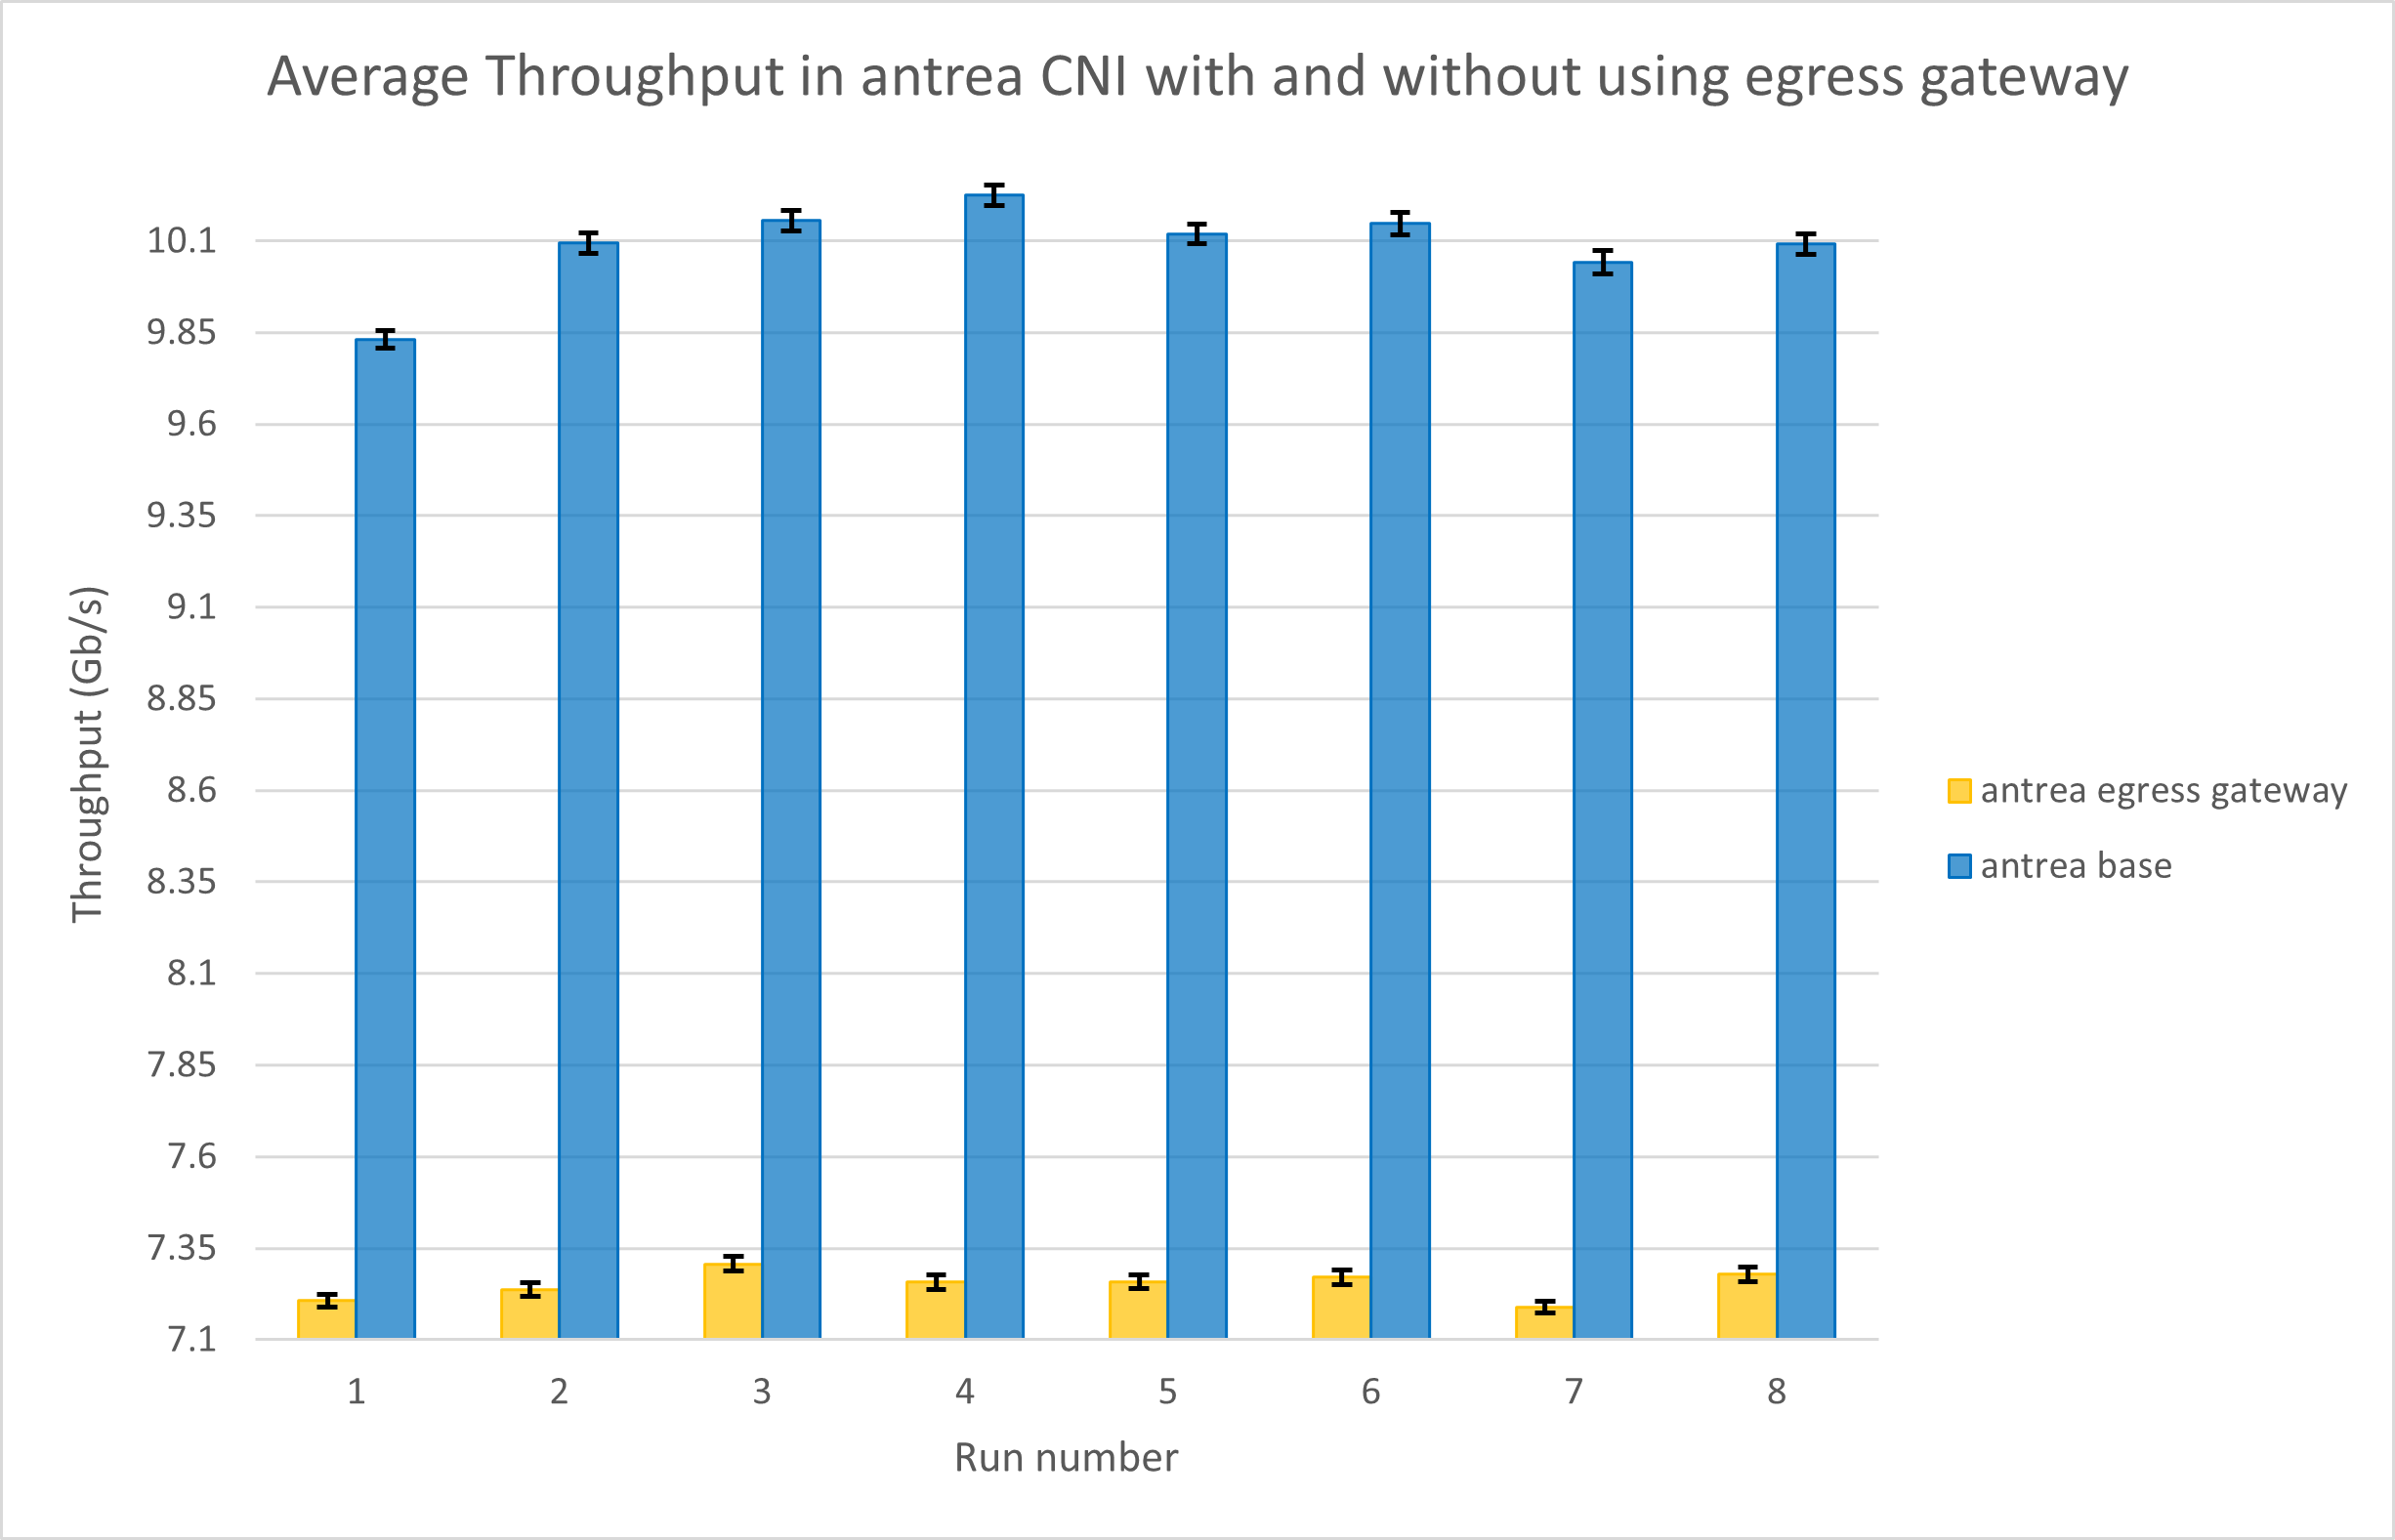
\includegraphics[width=\textwidth]{plots/small/throughput_antrea.png}
        \caption{}
        \label{fig:throughput_c}
    \end{subfigure}
    \hfill
    \begin{subfigure}[b]{0.45\textwidth}
        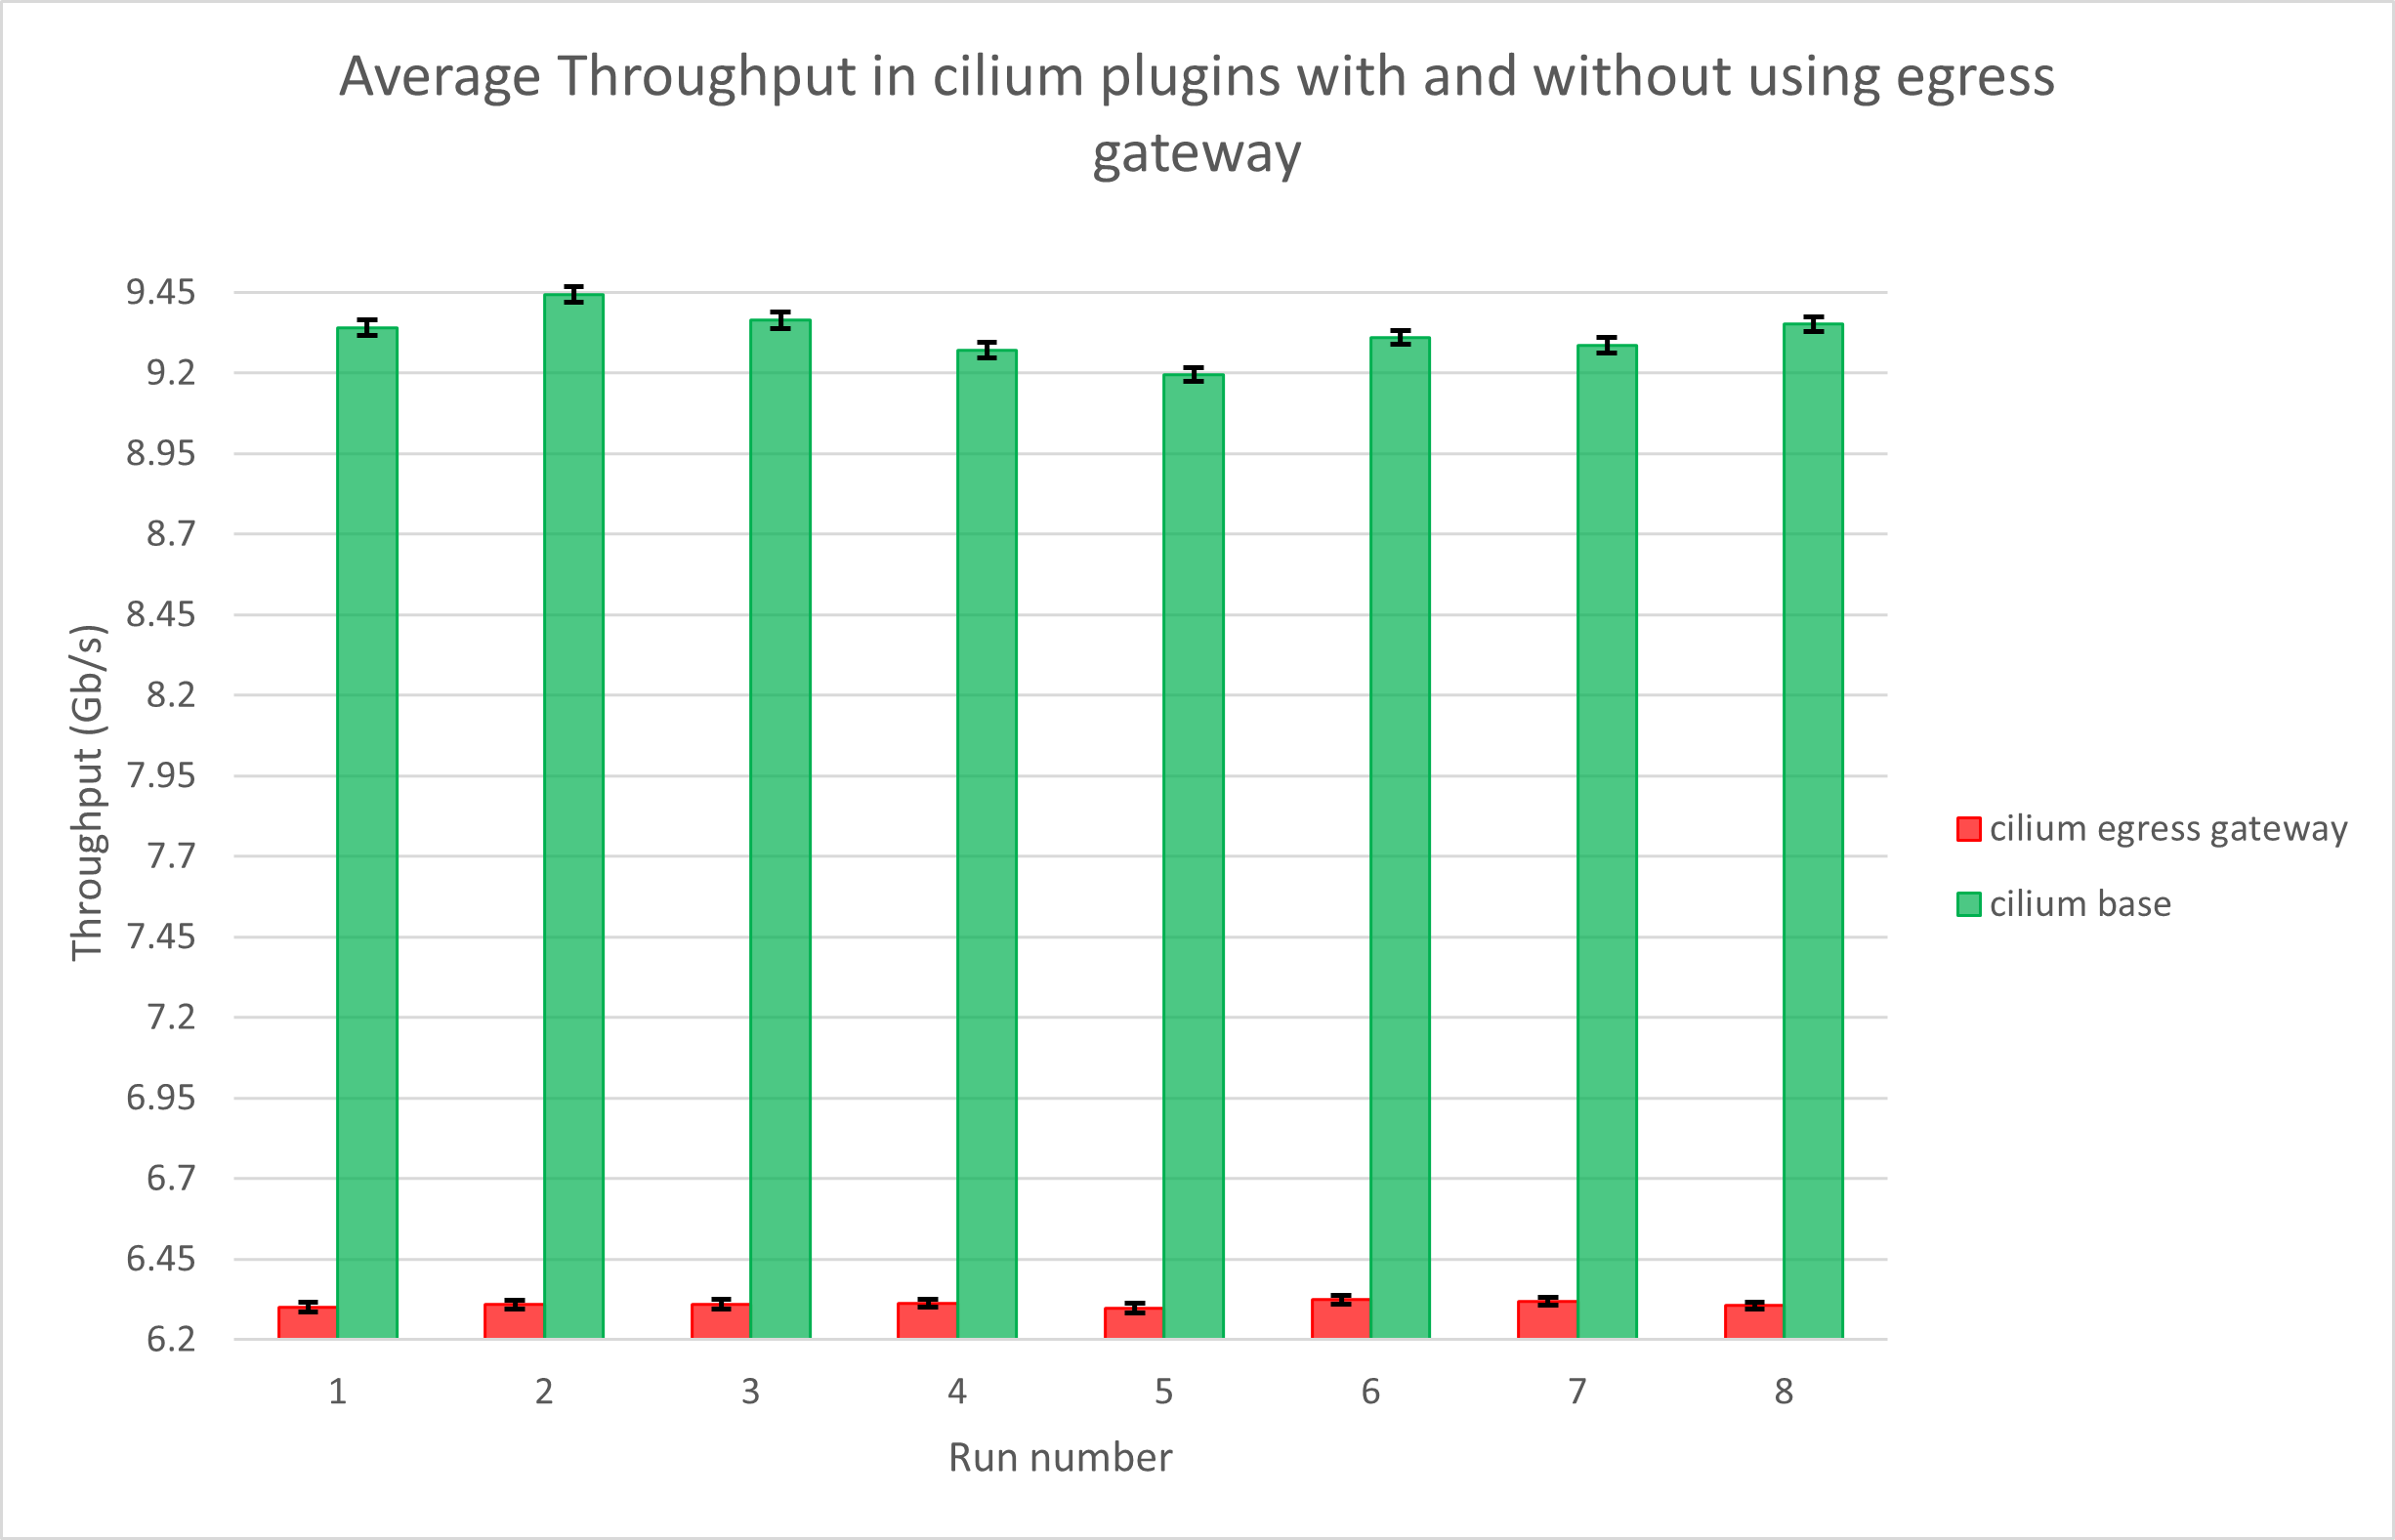
\includegraphics[width=\textwidth]{plots/small/throughput_cilium.png}
        \caption{}
        \label{fig:throughput_d}
    \end{subfigure}
    
    \caption{Throughput in all four test cases.}
    \label{fig:throughFour}
\end{figure}

\begin{figure}[H]
    \centering
    \begin{subfigure}[b]{0.45\textwidth}
        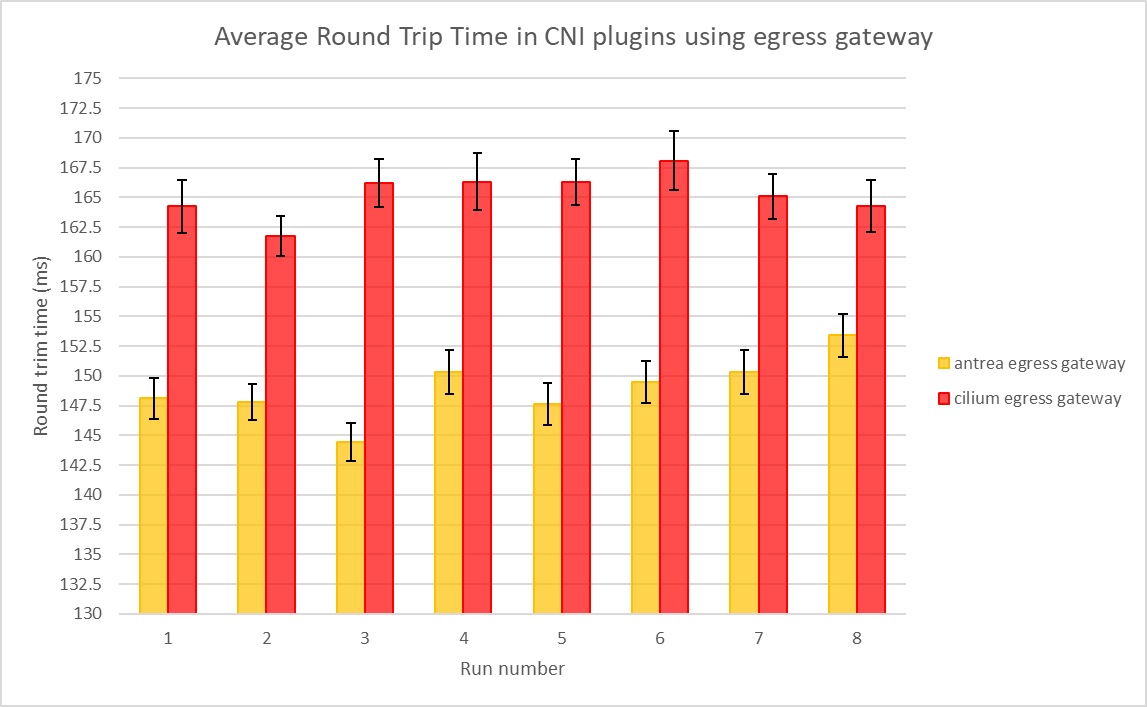
\includegraphics[width=\textwidth]{plots/small/rtt_egress.png}
        \caption{}
        \label{fig:rtt_a}
    \end{subfigure}
    \hfill
    \begin{subfigure}[b]{0.45\textwidth}
        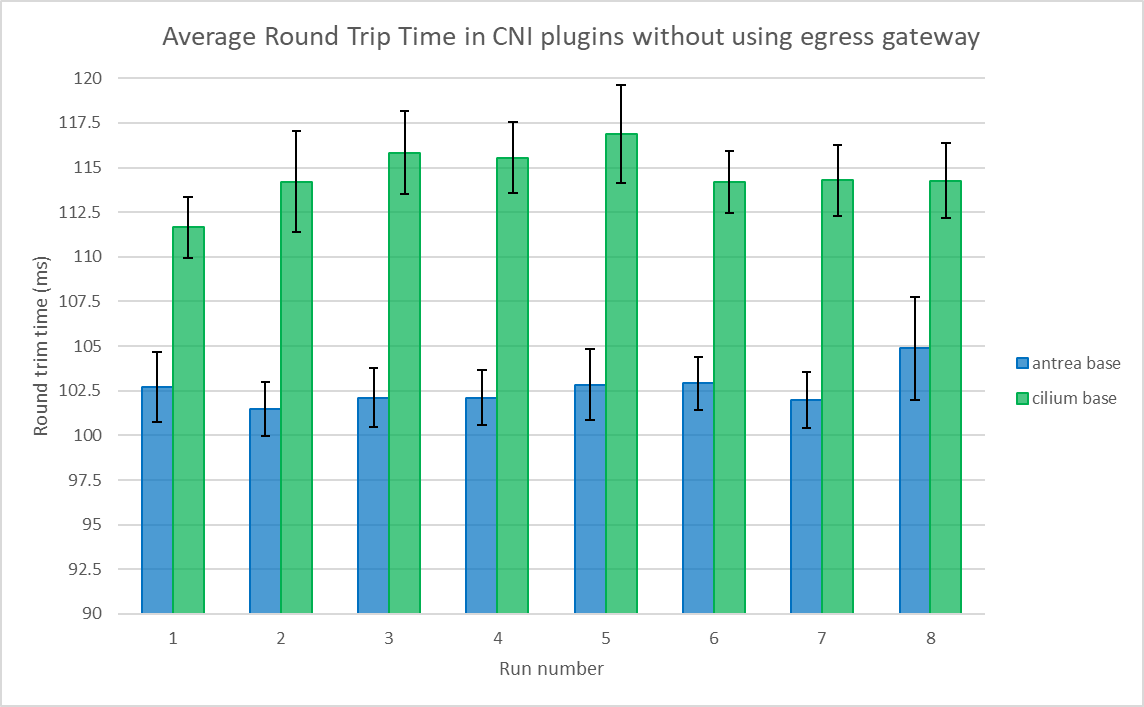
\includegraphics[width=\textwidth]{plots/small/rtt_base.png}
        \caption{}
        \label{fig:rtt_b}
    \end{subfigure}
    
    \vspace{10pt}
    
    \begin{subfigure}[b]{0.45\textwidth}
        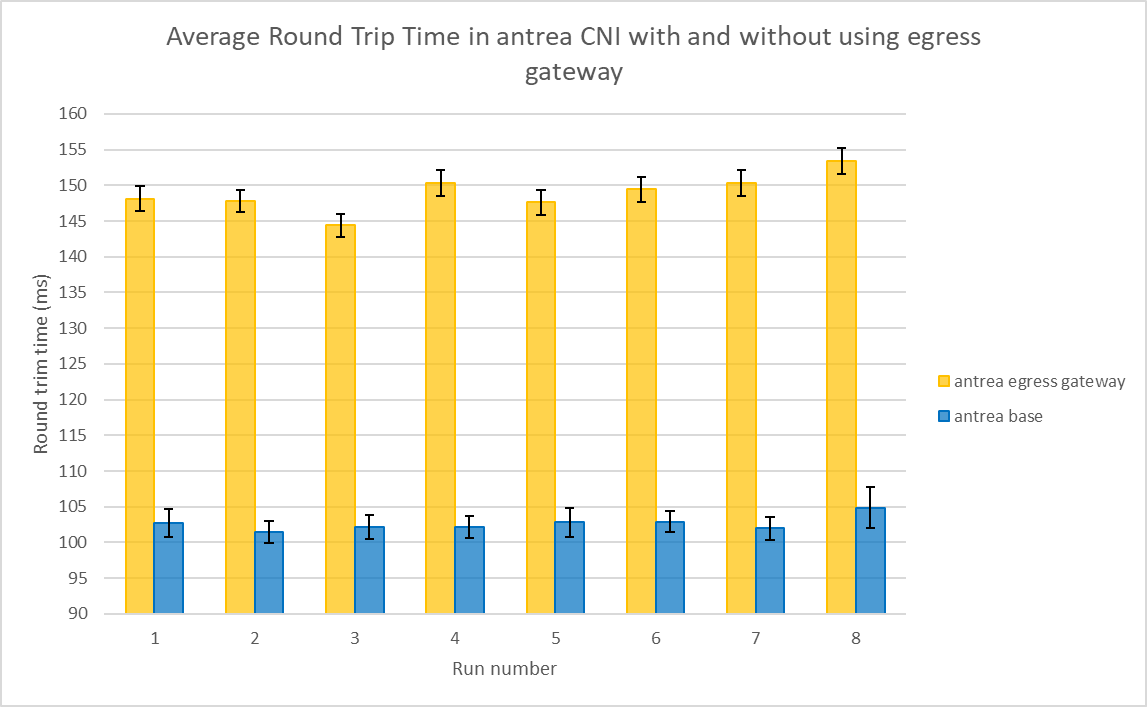
\includegraphics[width=\textwidth]{plots/small/rtt_antrea.png}
        \caption{}
        \label{fig:rtt_c}
    \end{subfigure}
    \hfill
    \begin{subfigure}[b]{0.45\textwidth}
        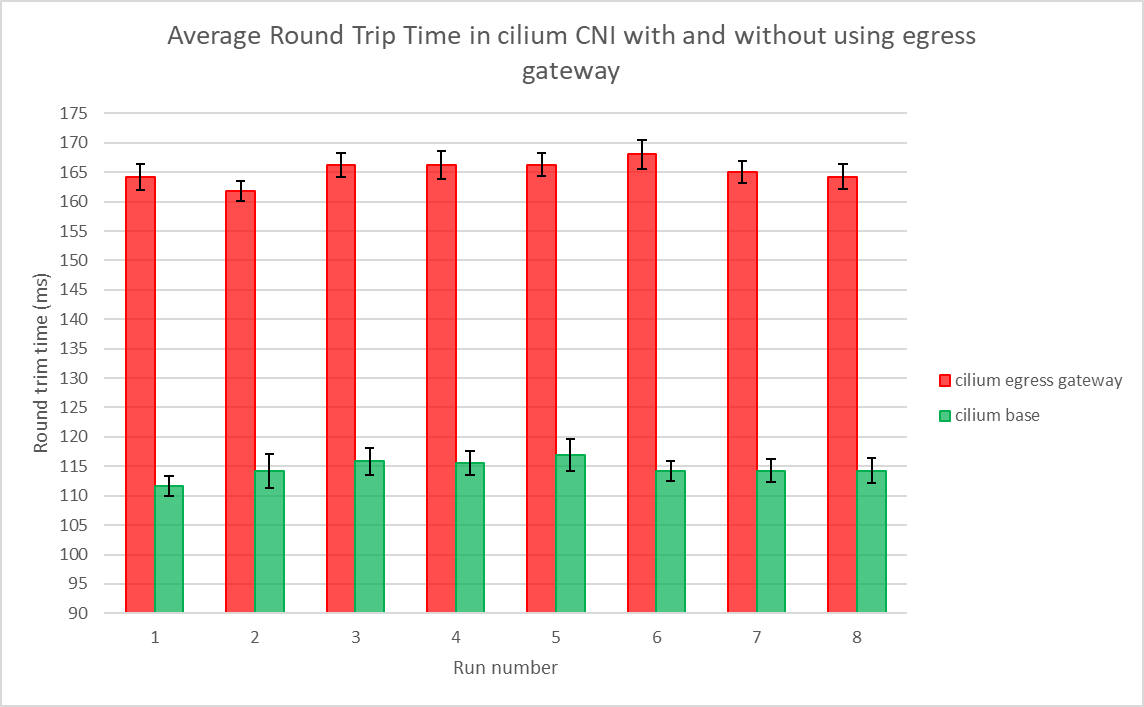
\includegraphics[width=\textwidth]{plots/small/rtt_cilium.png}
        \caption{}
        \label{fig:rtt_d}
    \end{subfigure}
    
    \caption{Round Trip Time in all four test cases.}
    \label{fig:rttFour}
\end{figure}

\section{Ingress Scenario}
\label{sec:ingressComparison}

\subsubsection{Resource consumption}
\label{sec:ingressResoureComsumption}


\begin{figure}[H]
    \centering
    \begin{subfigure}[b]{0.8\textwidth}
        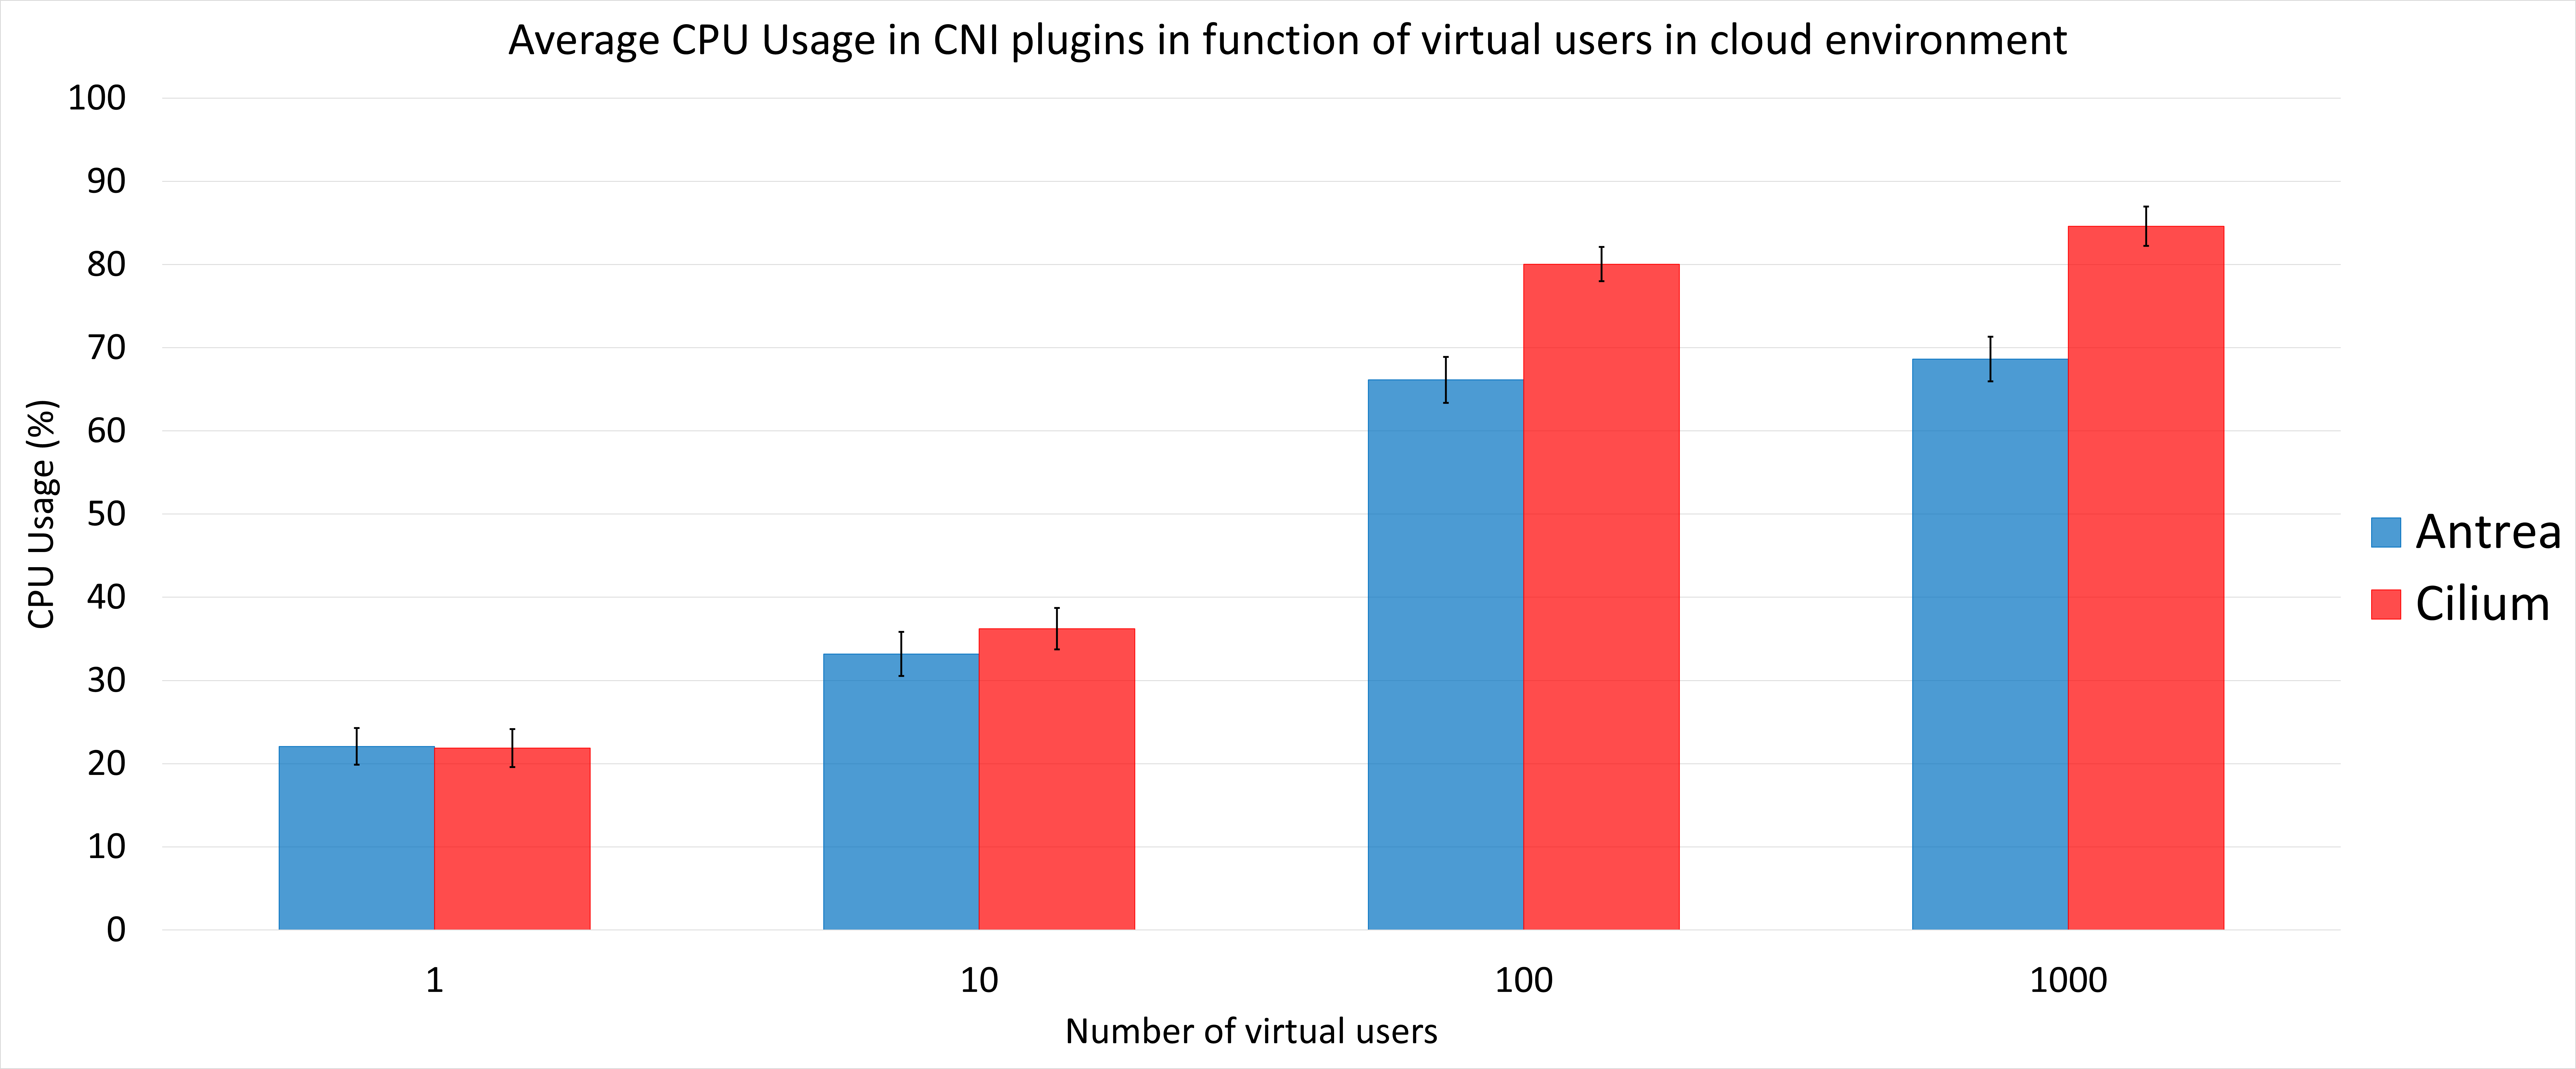
\includegraphics[width=\textwidth]{plots/traffic-splitting/cpu_cloud.png}
        \caption{}
        \label{fig:cpu_cloud_avg}
    \end{subfigure}
    \begin{subfigure}[b]{0.8\textwidth}
        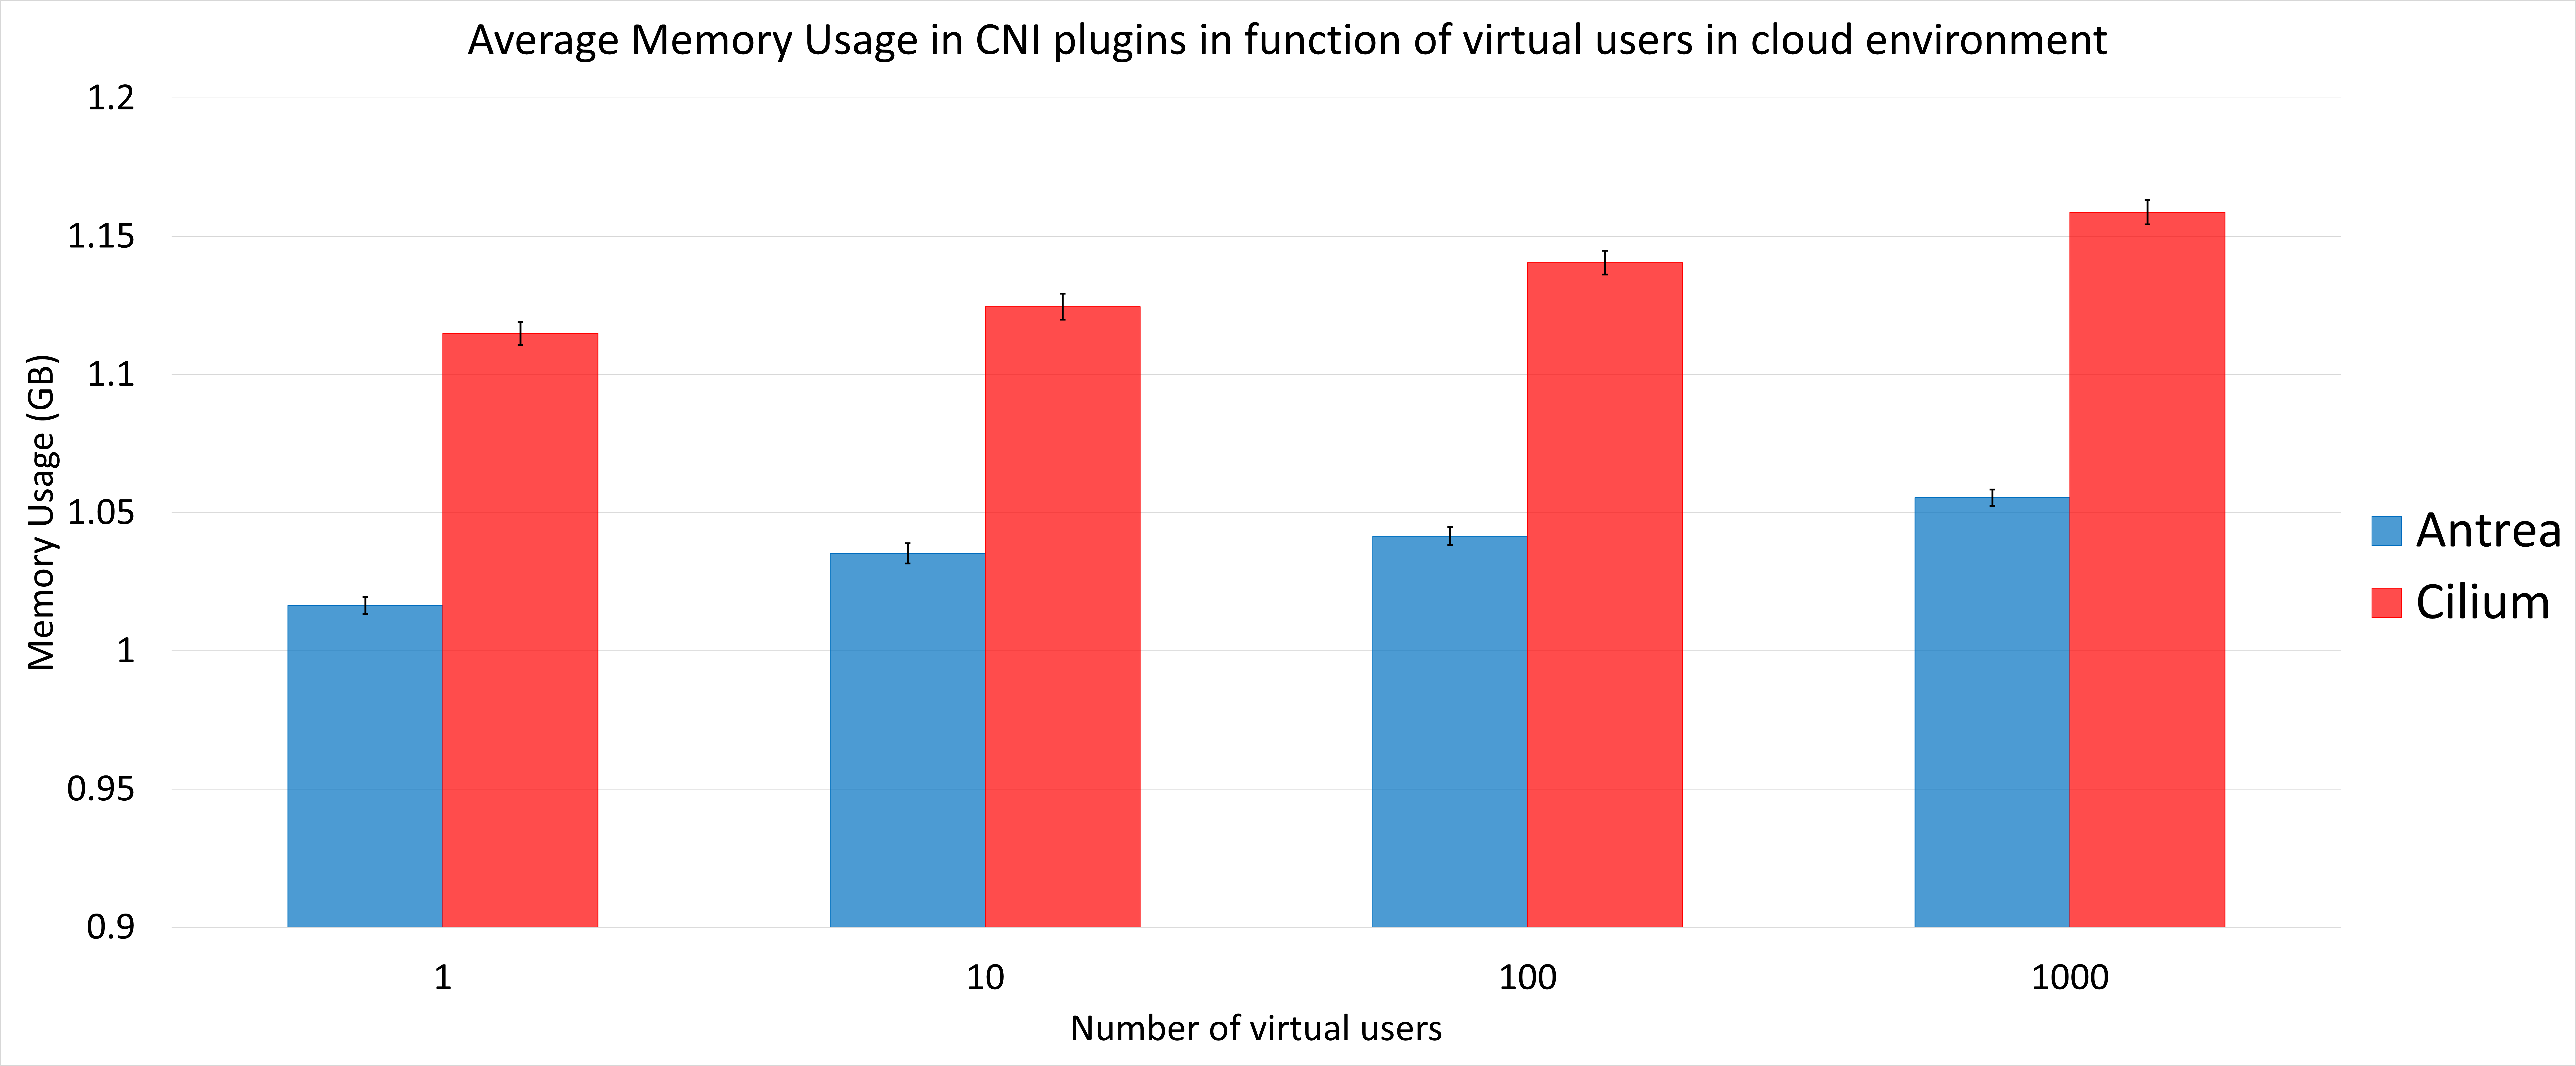
\includegraphics[width=\textwidth]{plots/traffic-splitting/memory_cloud.png}
        \caption{}
        \label{fig:memory_cloud_avg}
    \end{subfigure}
    
    \caption{Average resource utilization in ingress scenario with increasing virtual users in cloud environment, (a) CPU, (b) Memory}
    \label{fig:resource_cloud_avg}
\end{figure}

\begin{figure}[H]
    \centering
    \begin{subfigure}[b]{0.8\textwidth}
        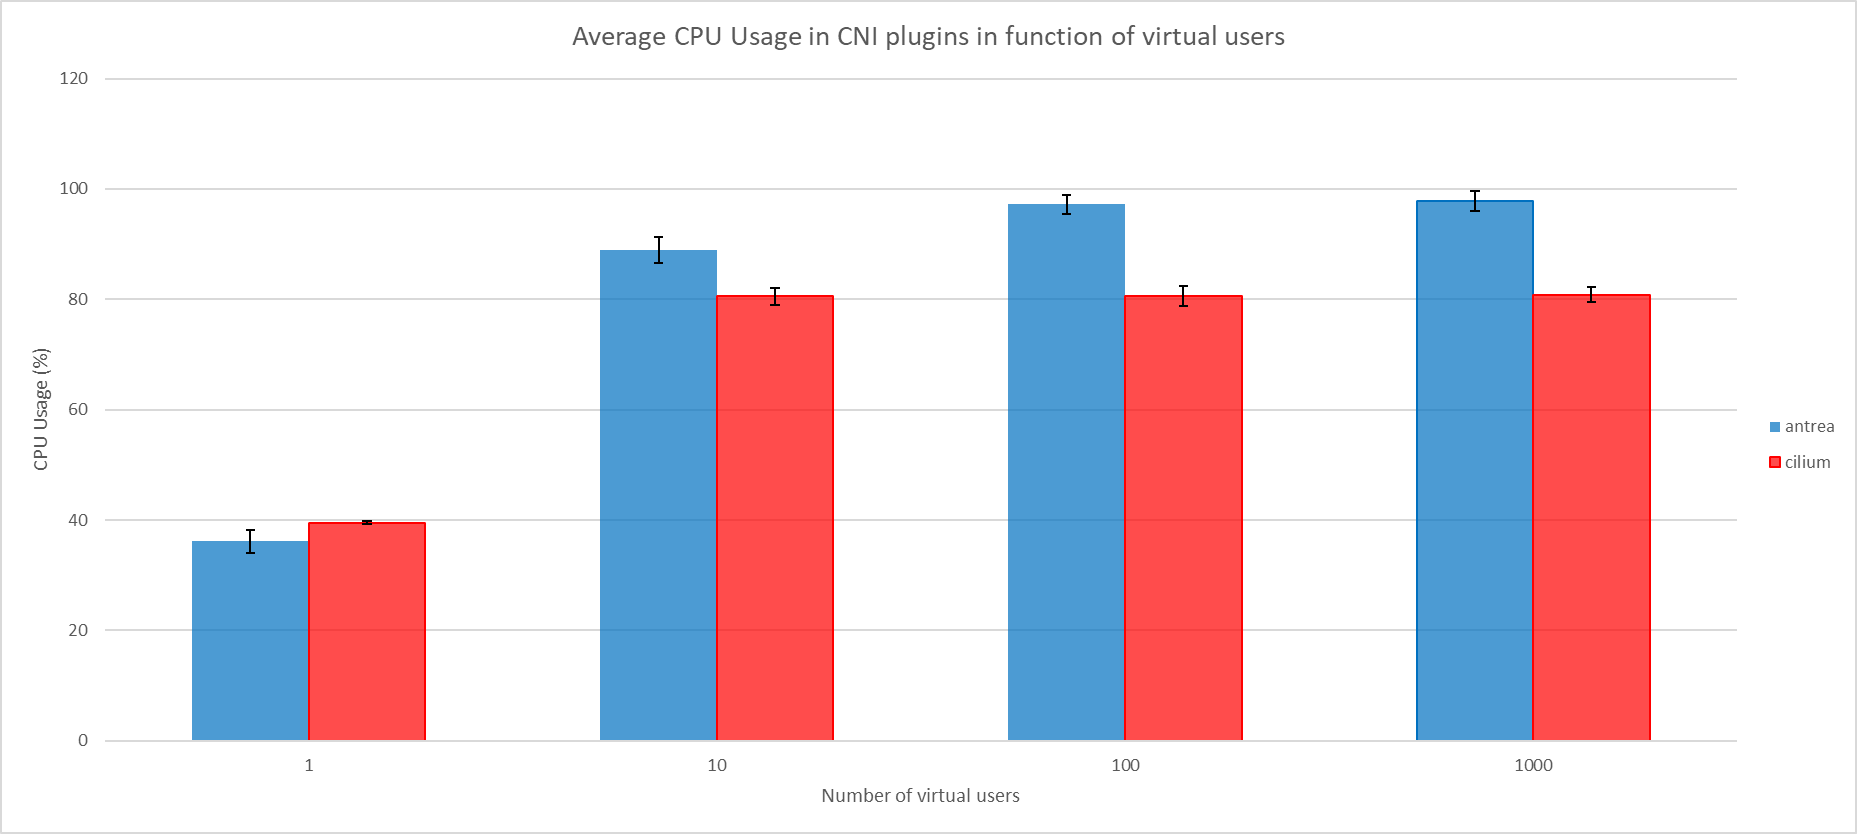
\includegraphics[width=\textwidth]{plots/traffic-splitting/cpu_local.png}
        \caption{}
        \label{fig:cpu_local_avg}
    \end{subfigure}
    \begin{subfigure}[b]{0.8\textwidth}
        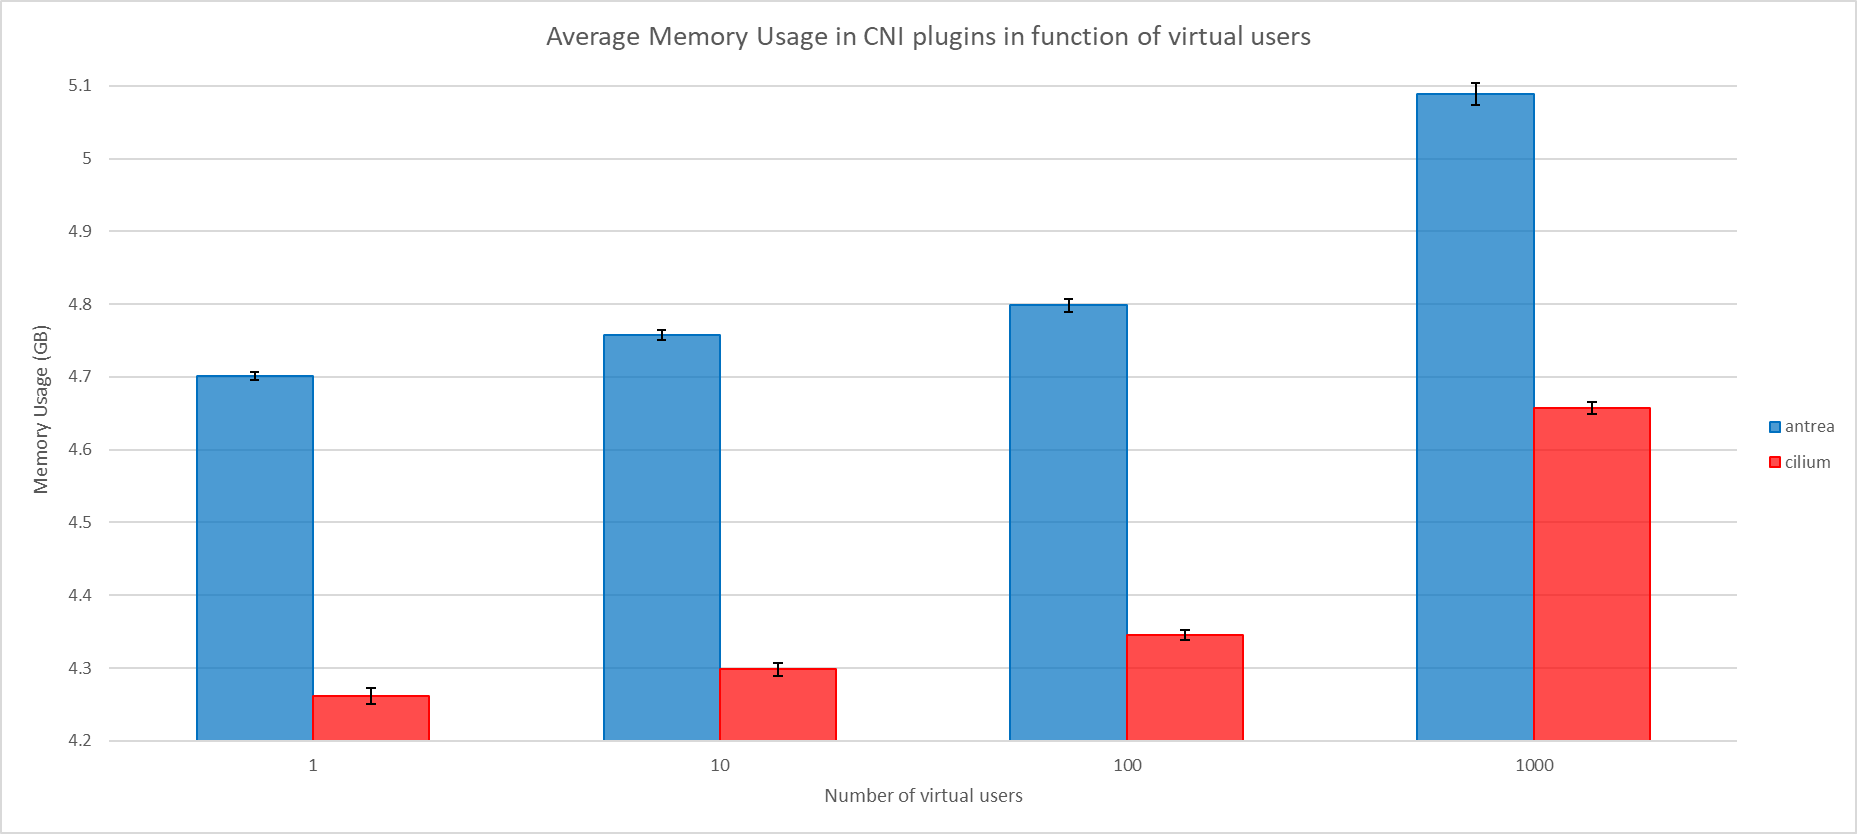
\includegraphics[width=\textwidth]{plots/traffic-splitting/memory_local.png}
        \caption{}
        \label{fig:memory_local_avg}
    \end{subfigure}
    
    \caption{Average resource utilization in ingress scenario with increasing virtual users in local environment, (a) CPU, (b) Memory}
    \label{fig:resource_local_avg}
\end{figure}

Comparing Figures~\ref{fig:resource_cloud_avg} and~\ref{fig:resource_local_avg}, it is evident that traffic management primarily impacts CPU usage rather than memory consumption, as the memory usage shows lower increases. In the cloud environment, Antrea demonstrates better resource efficiency, whereas in the cloud environment, Cilium consumes less resources.


\begin{figure}[H]
    \centering
    \begin{subfigure}[b]{0.8\textwidth}
        
\includegraphics[width=\textwidth]{plots/traffic-splitting/vus_cloud_all.png}
        \caption{}
        \label{fig:vus_cloud_avg}
    \end{subfigure}
    \begin{subfigure}[b]{0.8\textwidth}
        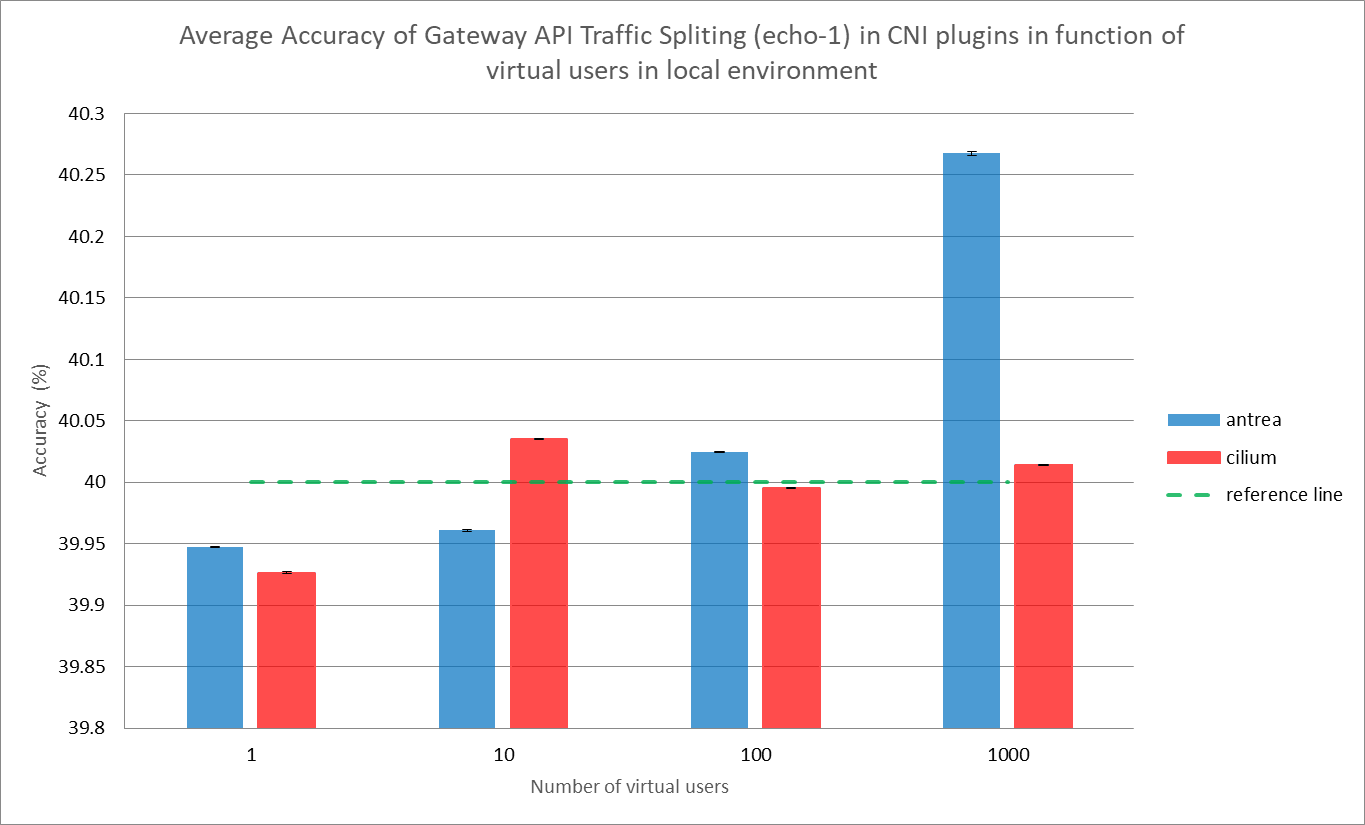
\includegraphics[width=\textwidth]{plots/traffic-splitting/vus_local_all.png}
        \caption{}
        \label{fig:vus_local_avg}
    \end{subfigure}
    
    \caption{Average traffic splitting accuracy in ingress scenario with increasing virtual users (a) Cloud, (b) Local}
    \label{fig:vus_avg}
\end{figure}

When comparing traffic weighting accuracy with an increasing number of virtual users in a cloud environment, antrea proves to be more precise both when a single user makes a request and when thousand users generate massive load. In a local environment, Cilium is more accurate in splitting traffic to a value specified in HTTPRoute in every scenario except for the case of a single user. Antrea in local environment has wider confidential intervals, and distance from reference point is high in comparison to cilium, making it less effective during high load period.

\begin{figure}[H]
    \centering
    \begin{subfigure}[b]{0.8\textwidth}
        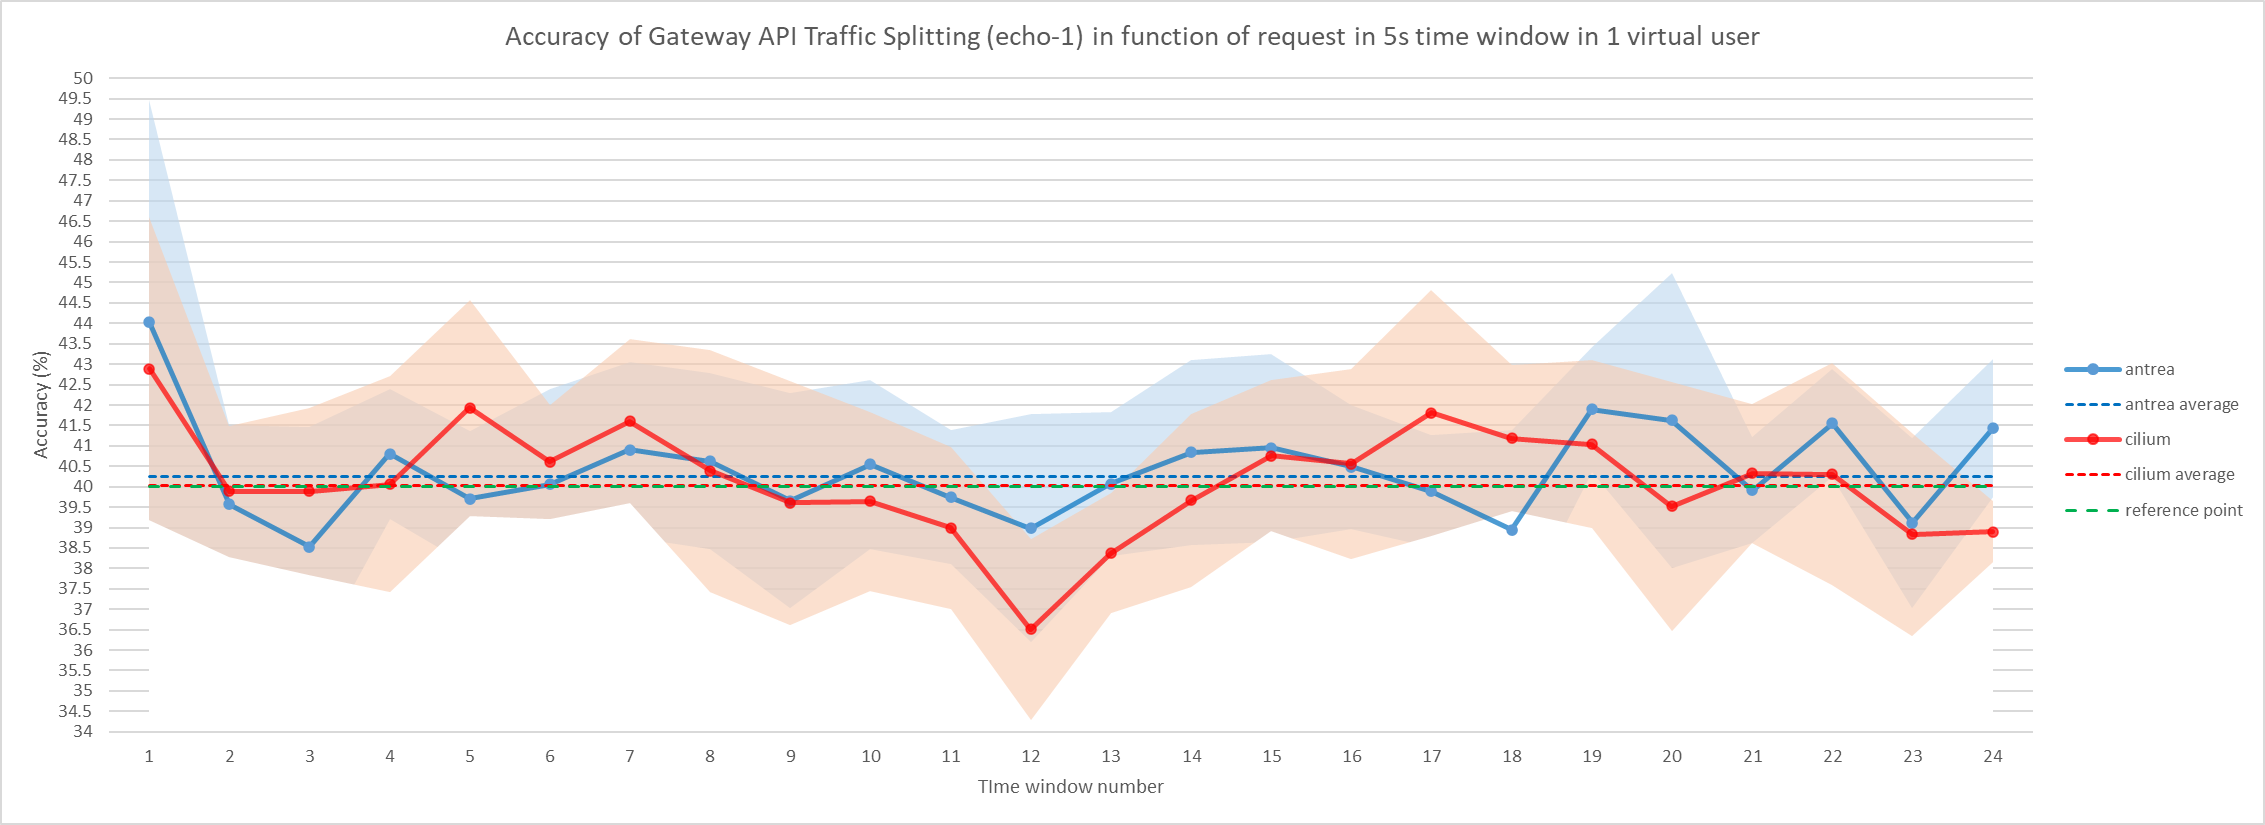
\includegraphics[width=\textwidth]{plots/traffic-splitting/time_window_5_1vu_cloud.png}
        \label{fig:time_window_1vu}
    \end{subfigure}

    \vspace{-0.1cm} % Adjusted minimal space between subfigures

    \begin{subfigure}[b]{0.8\textwidth}
        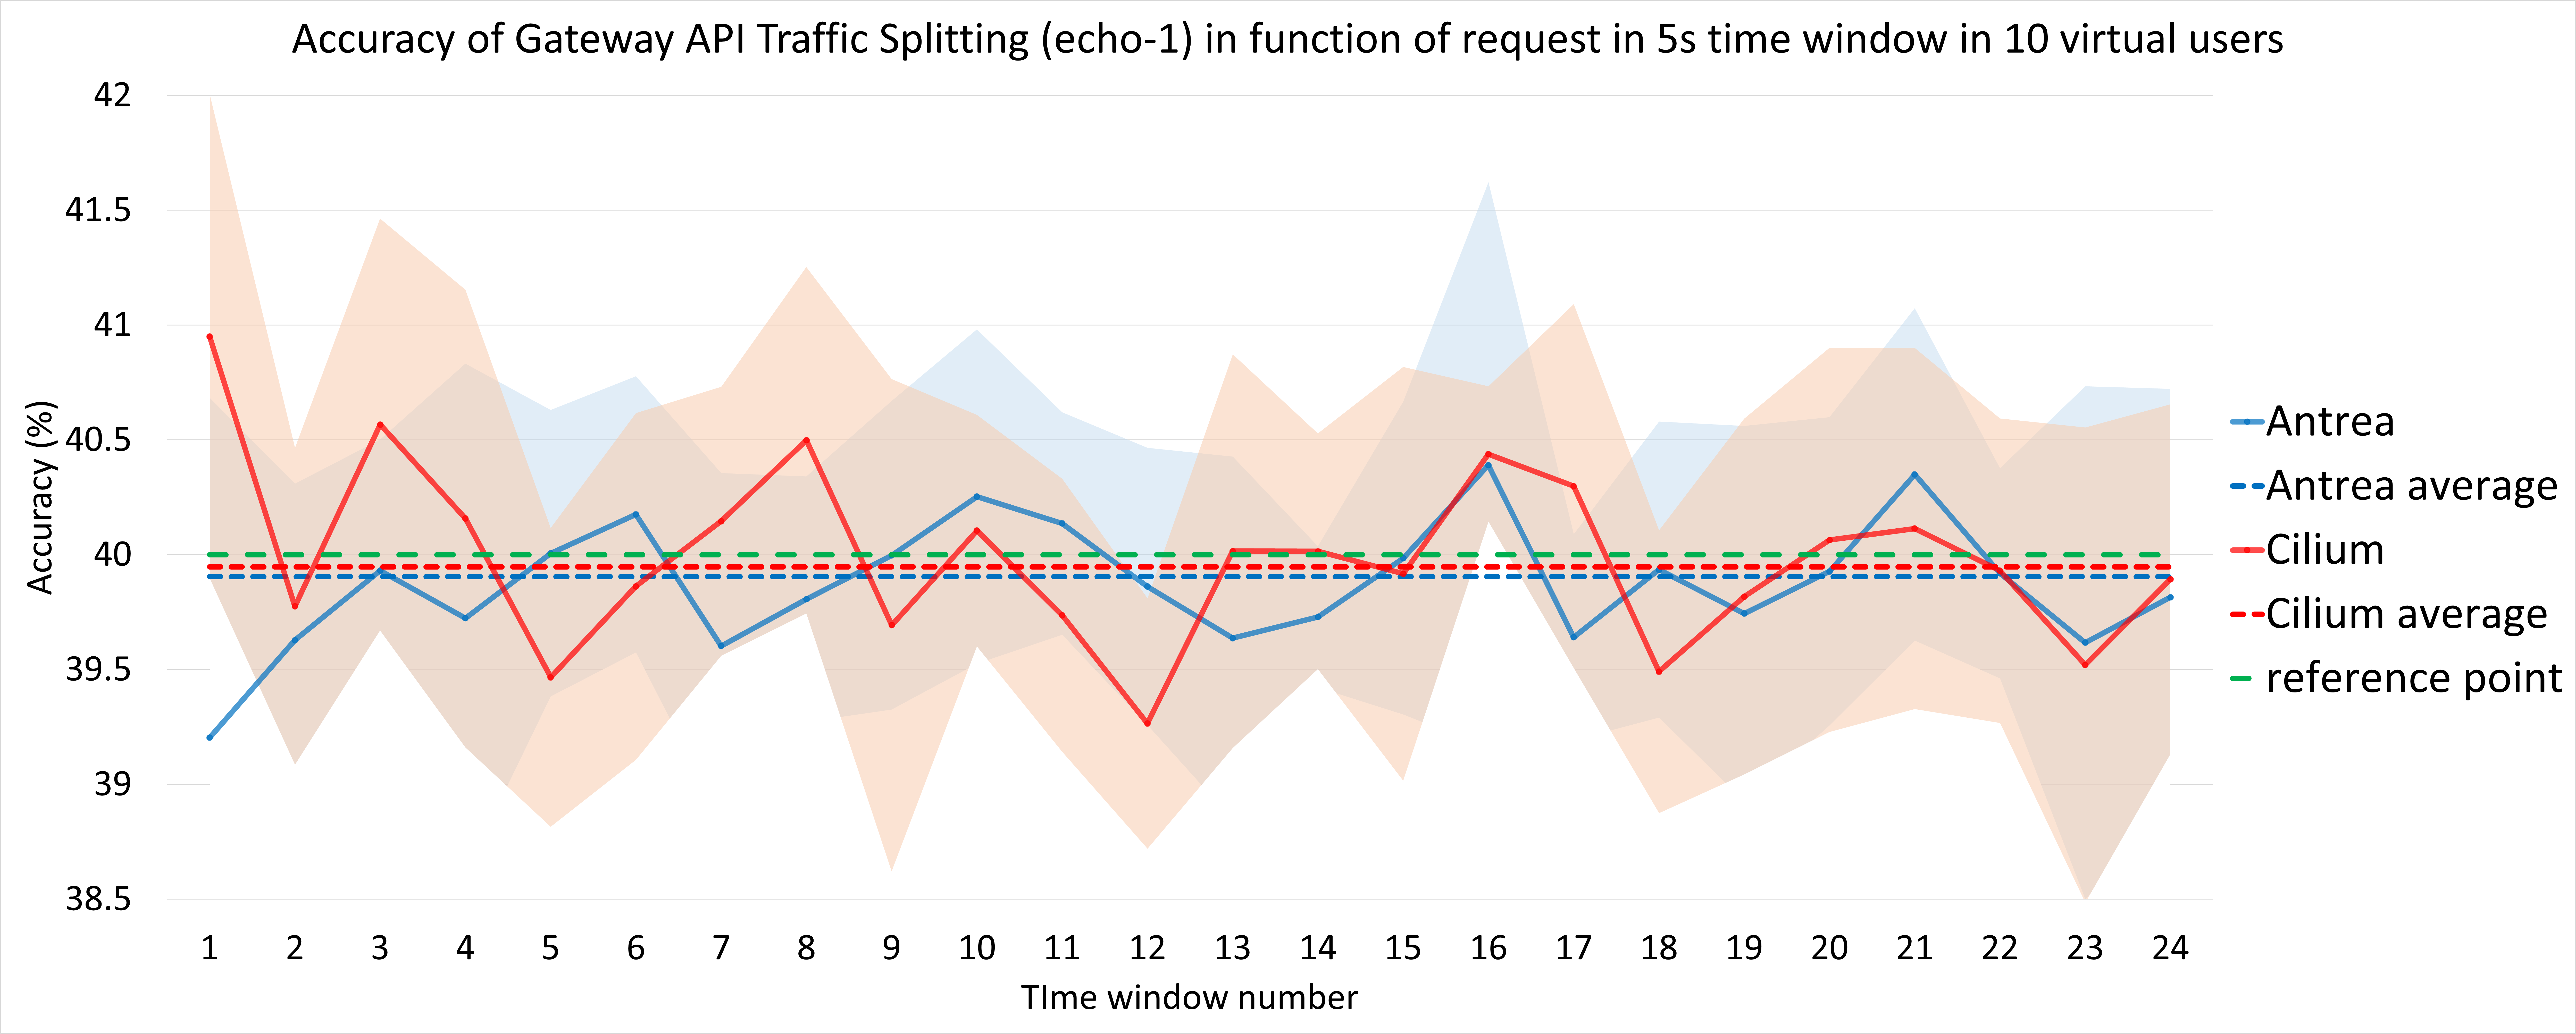
\includegraphics[width=\textwidth]{plots/traffic-splitting/time_window_5_10vu_cloud.png}
        \label{fig:time_window_10vu}
    \end{subfigure}

    \vspace{-0.1cm} % Adjusted minimal space between subfigures

    \begin{subfigure}[b]{0.8\textwidth}
        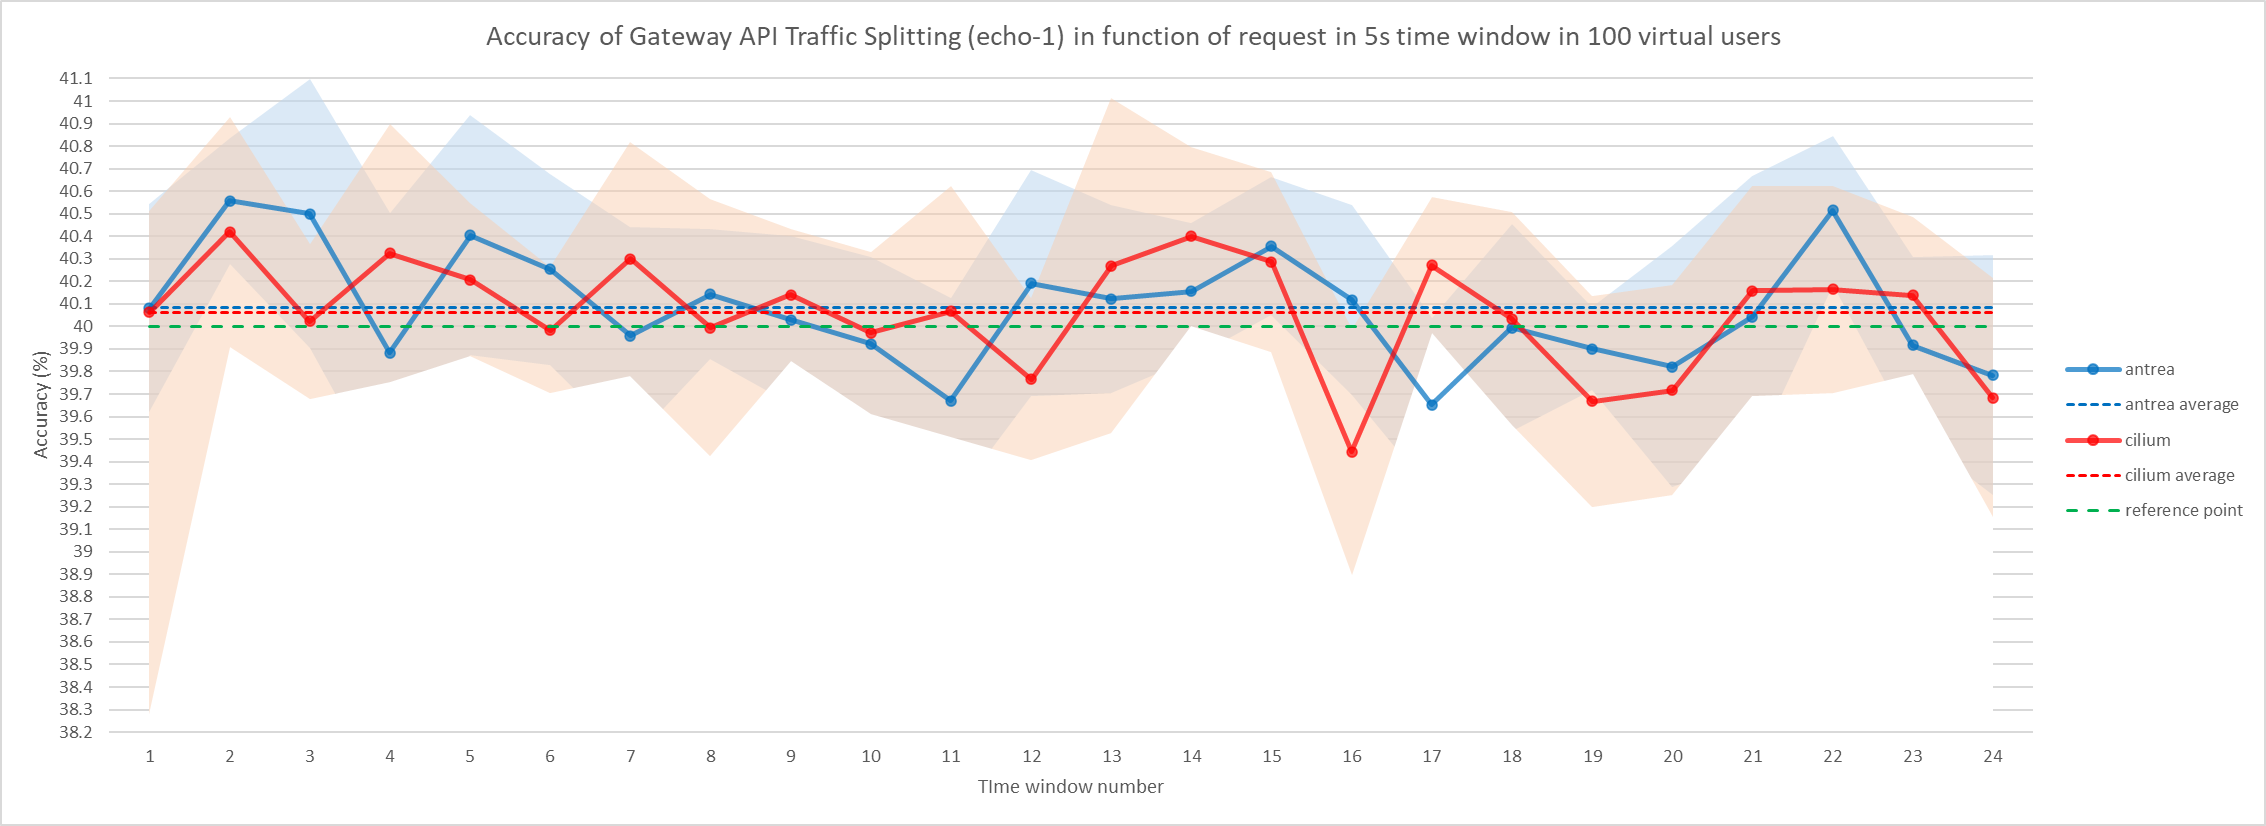
\includegraphics[width=\textwidth]{plots/traffic-splitting/time_window_5_100vu_cloud.png}
        \label{fig:time_window_100vu}
    \end{subfigure}

    \vspace{-0.1cm} % Adjusted minimal space between subfigures

    \begin{subfigure}[b]{0.8\textwidth}
        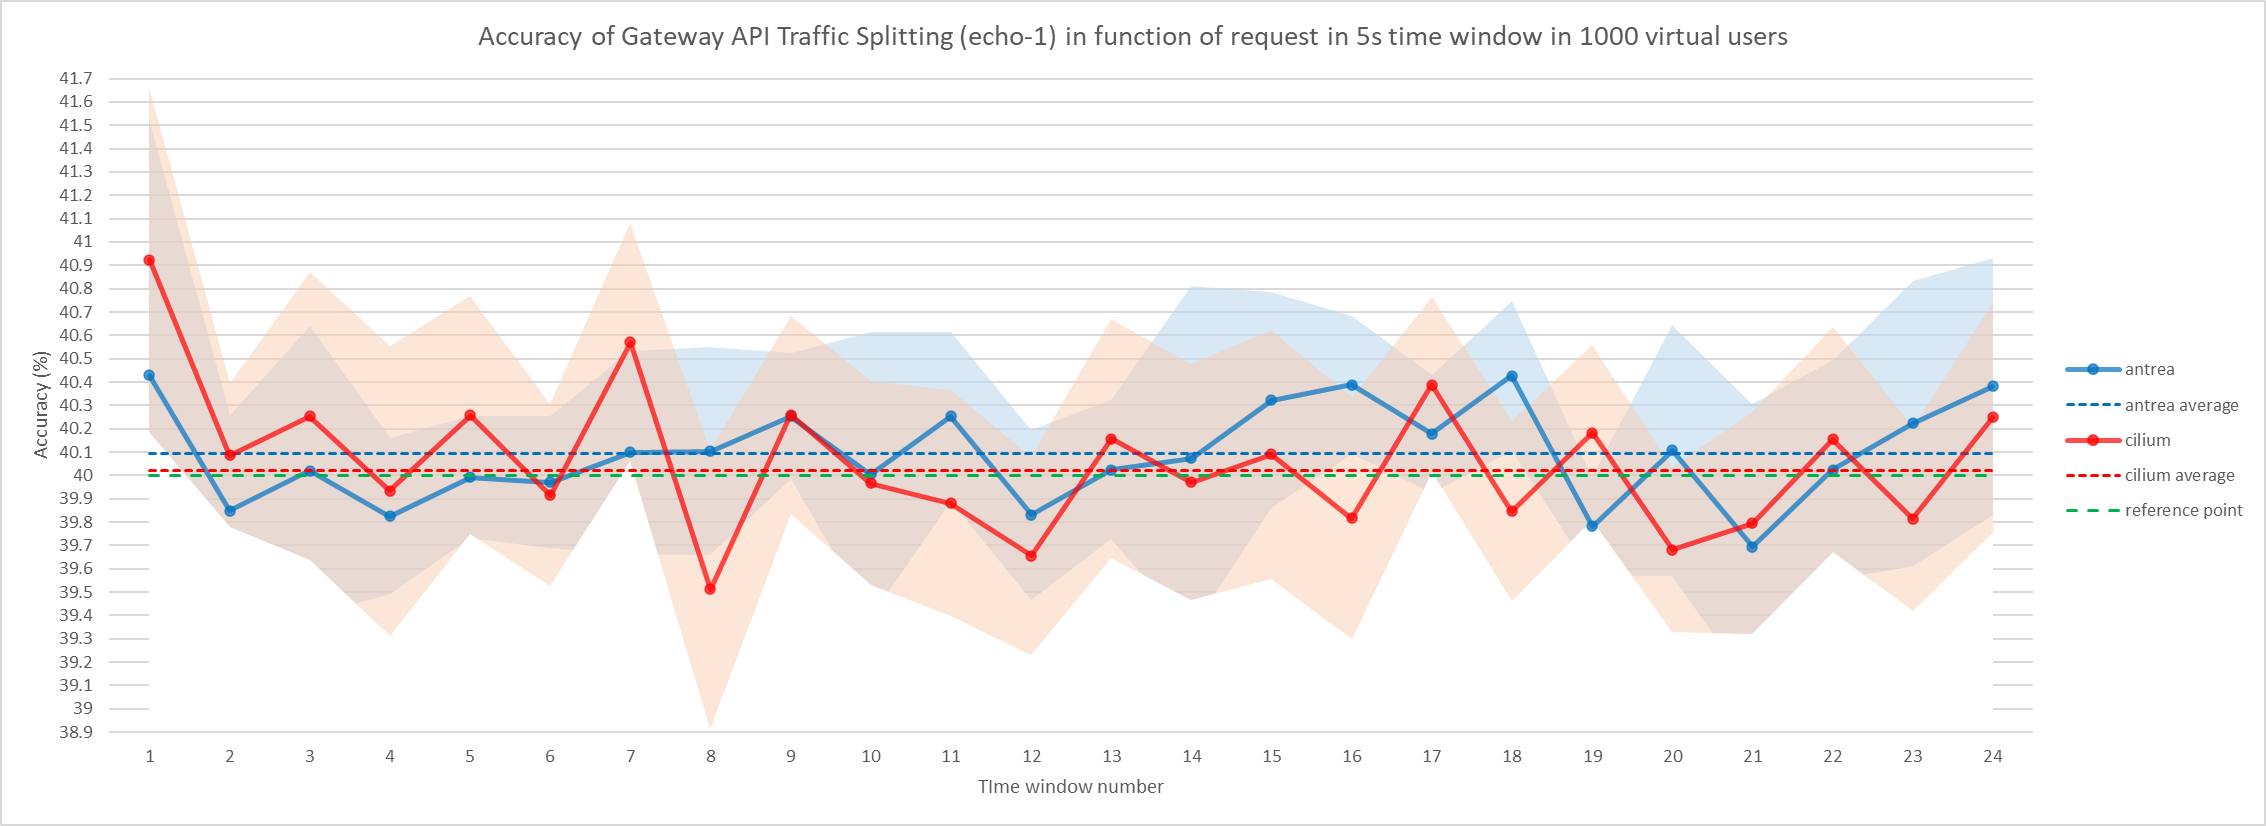
\includegraphics[width=\textwidth]{plots/traffic-splitting/time_window_5_1000vu_cloud.png}
        \label{fig:time_window_1000vu}
    \end{subfigure}

    \vspace{-0.3cm} % Reduced space between the last subfigure and the caption

    \caption{Average traffic splitting ratio in function of five second request time window with increasing virtual users; one, ten, houndred and tousand}
    \label{fig:avg_vus}
\end{figure}







\begin{figure}[H]
    \centering
    \begin{subfigure}[b]{0.48\textwidth}
        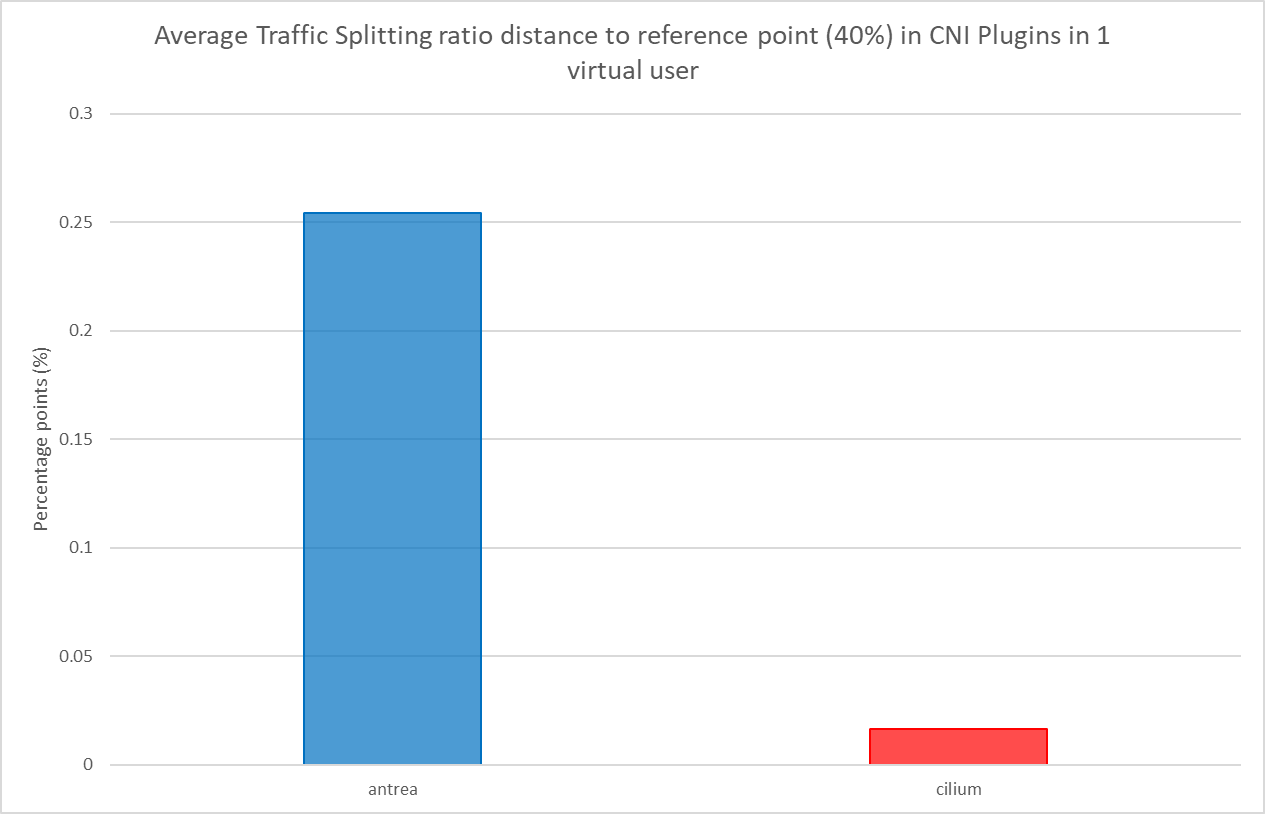
\includegraphics[width=\textwidth]{plots/traffic-splitting/time_window_5_1vu_reference_cloud.png}
        \label{fig:reference_1vu}
        \caption{}
    \end{subfigure}
    \begin{subfigure}[b]{0.48\textwidth}
        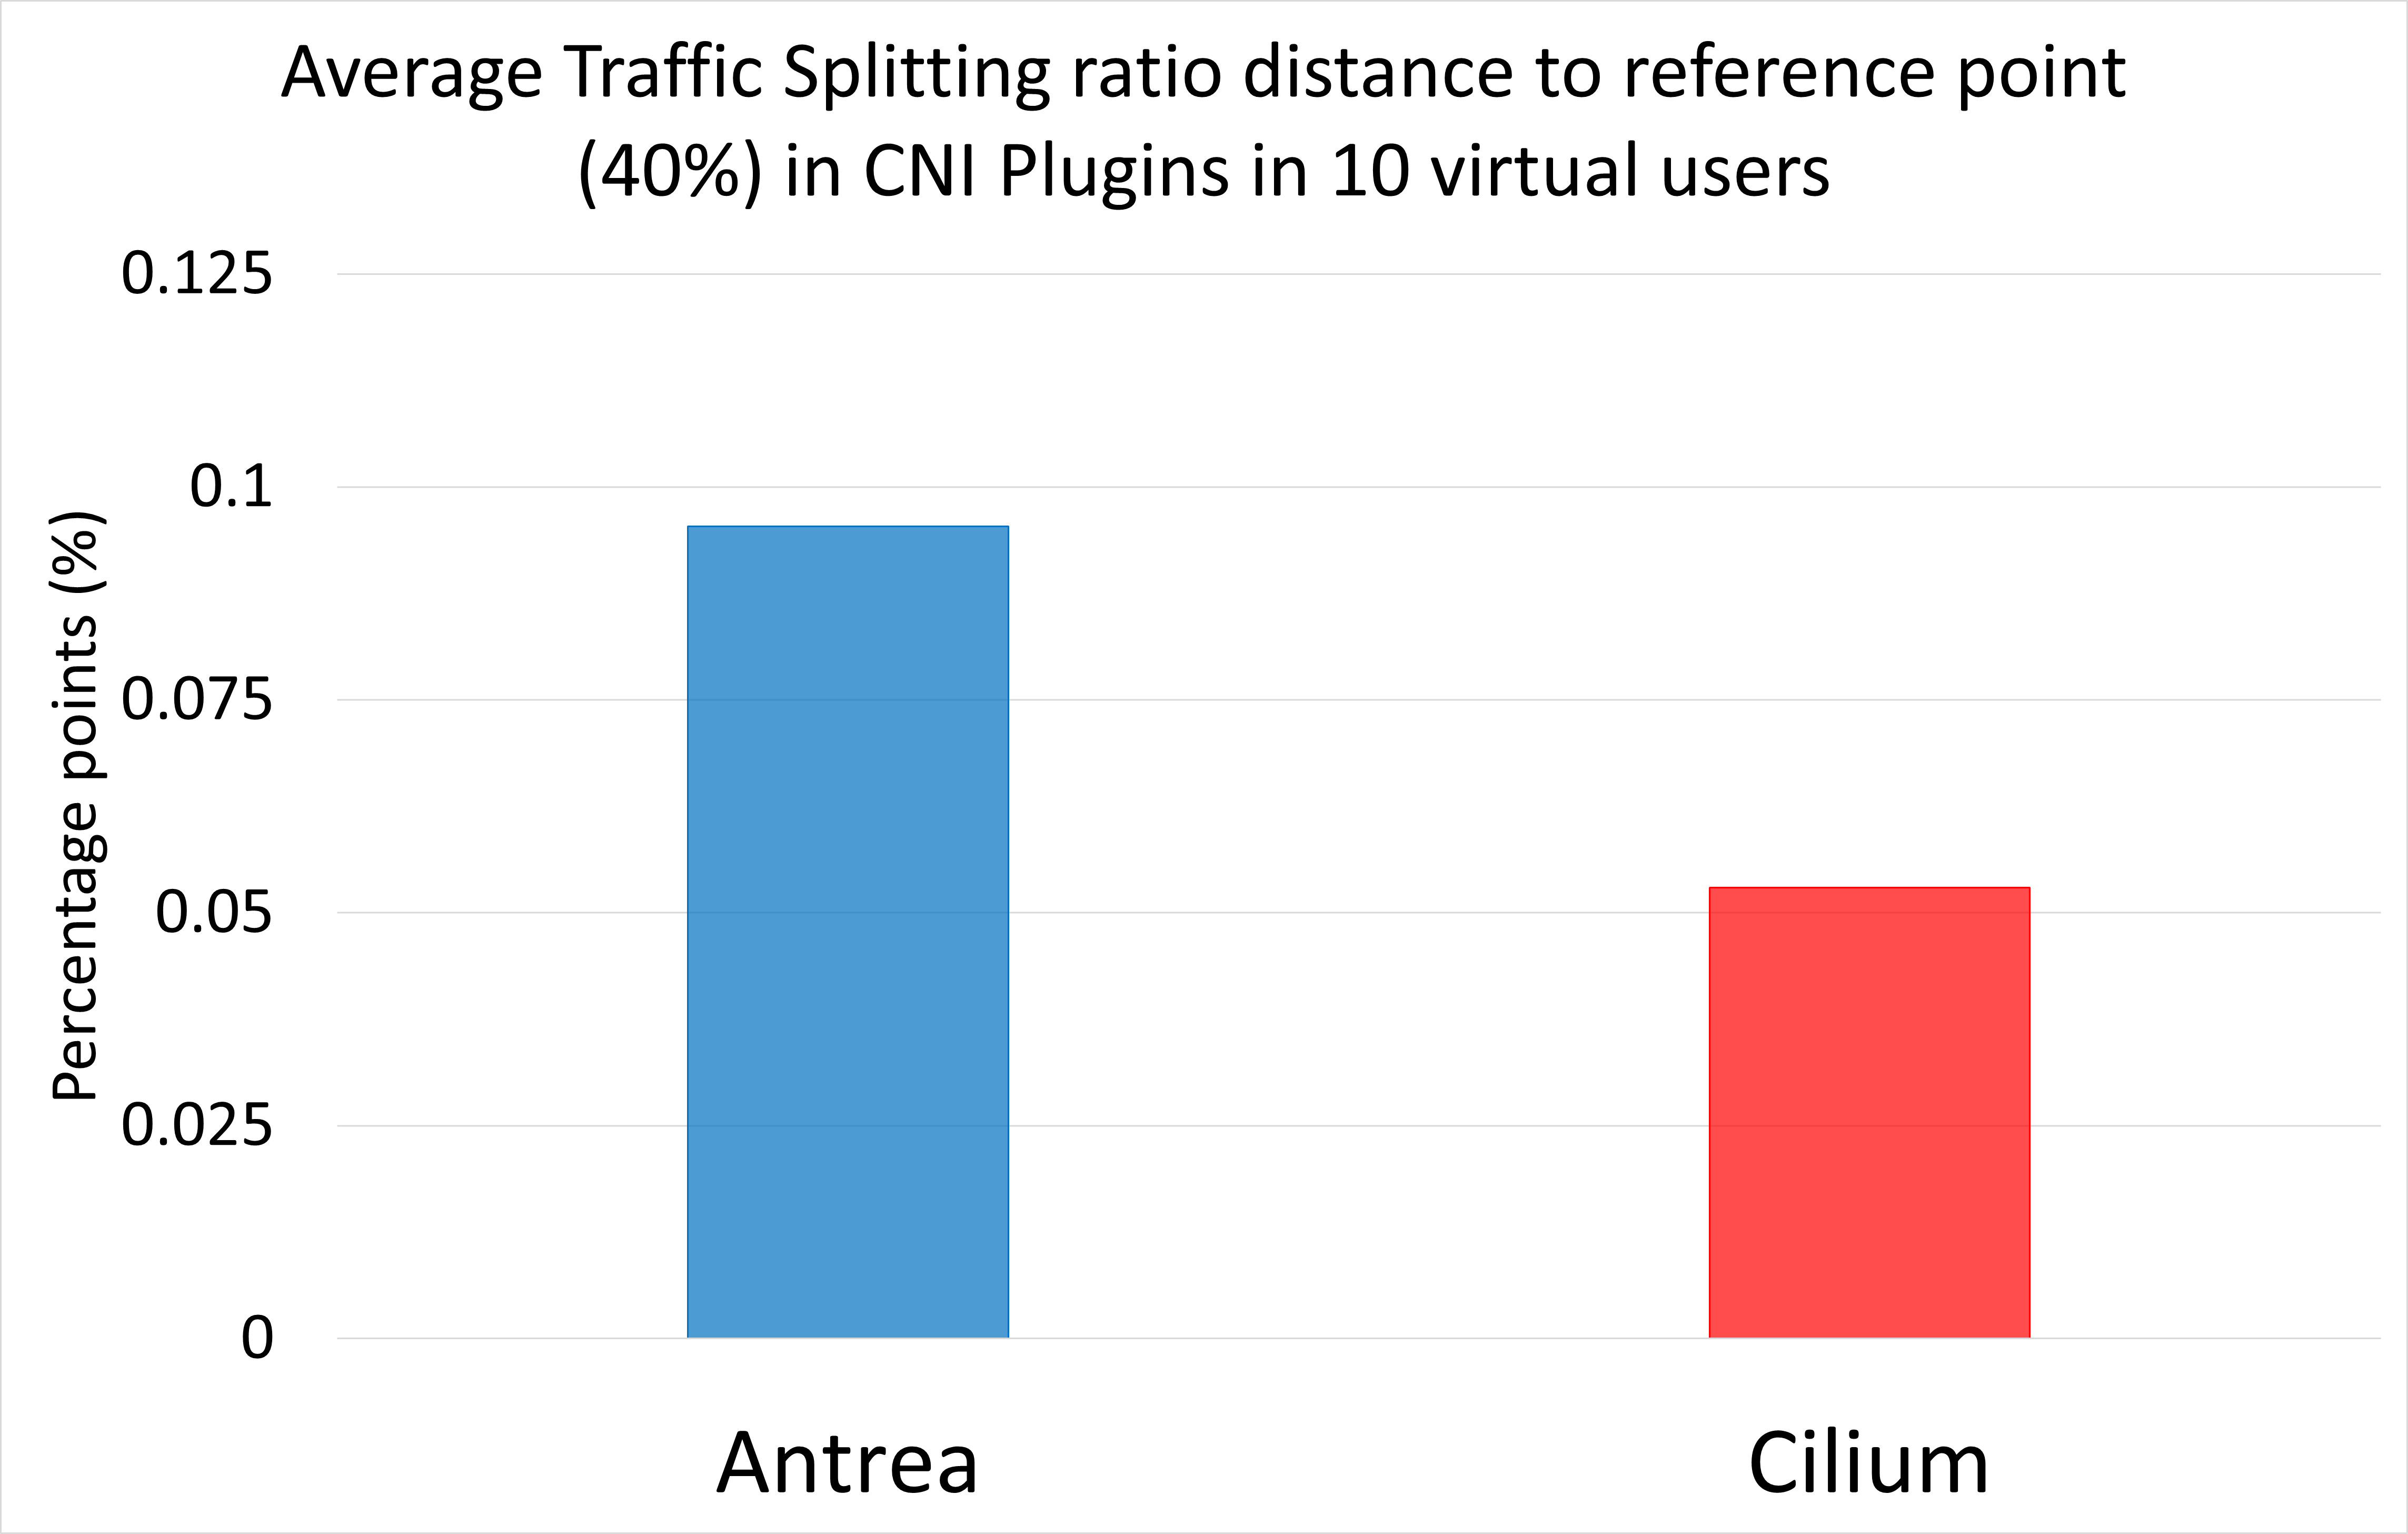
\includegraphics[width=\textwidth]{plots/traffic-splitting/time_window_5_10vu_reference_cloud.png}
        \label{fig:reference_10vu}
        \caption{}
    \end{subfigure}

    \vspace{0.5cm}

    \begin{subfigure}[b]{0.48\textwidth}
        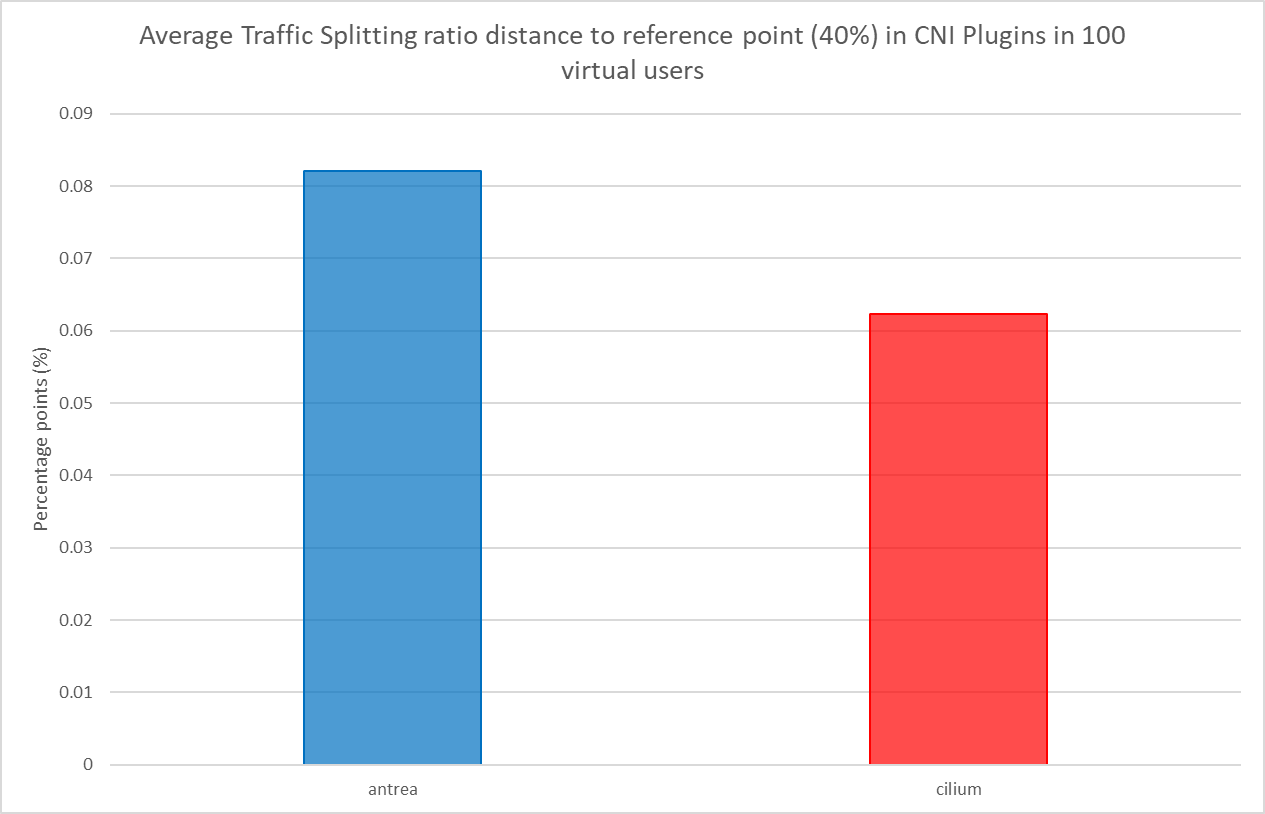
\includegraphics[width=\textwidth]{plots/traffic-splitting/time_window_5_100vu_reference_cloud.png}
        \label{fig:reference_100vu}
        \caption{}
    \end{subfigure}
    \begin{subfigure}[b]{0.48\textwidth}
        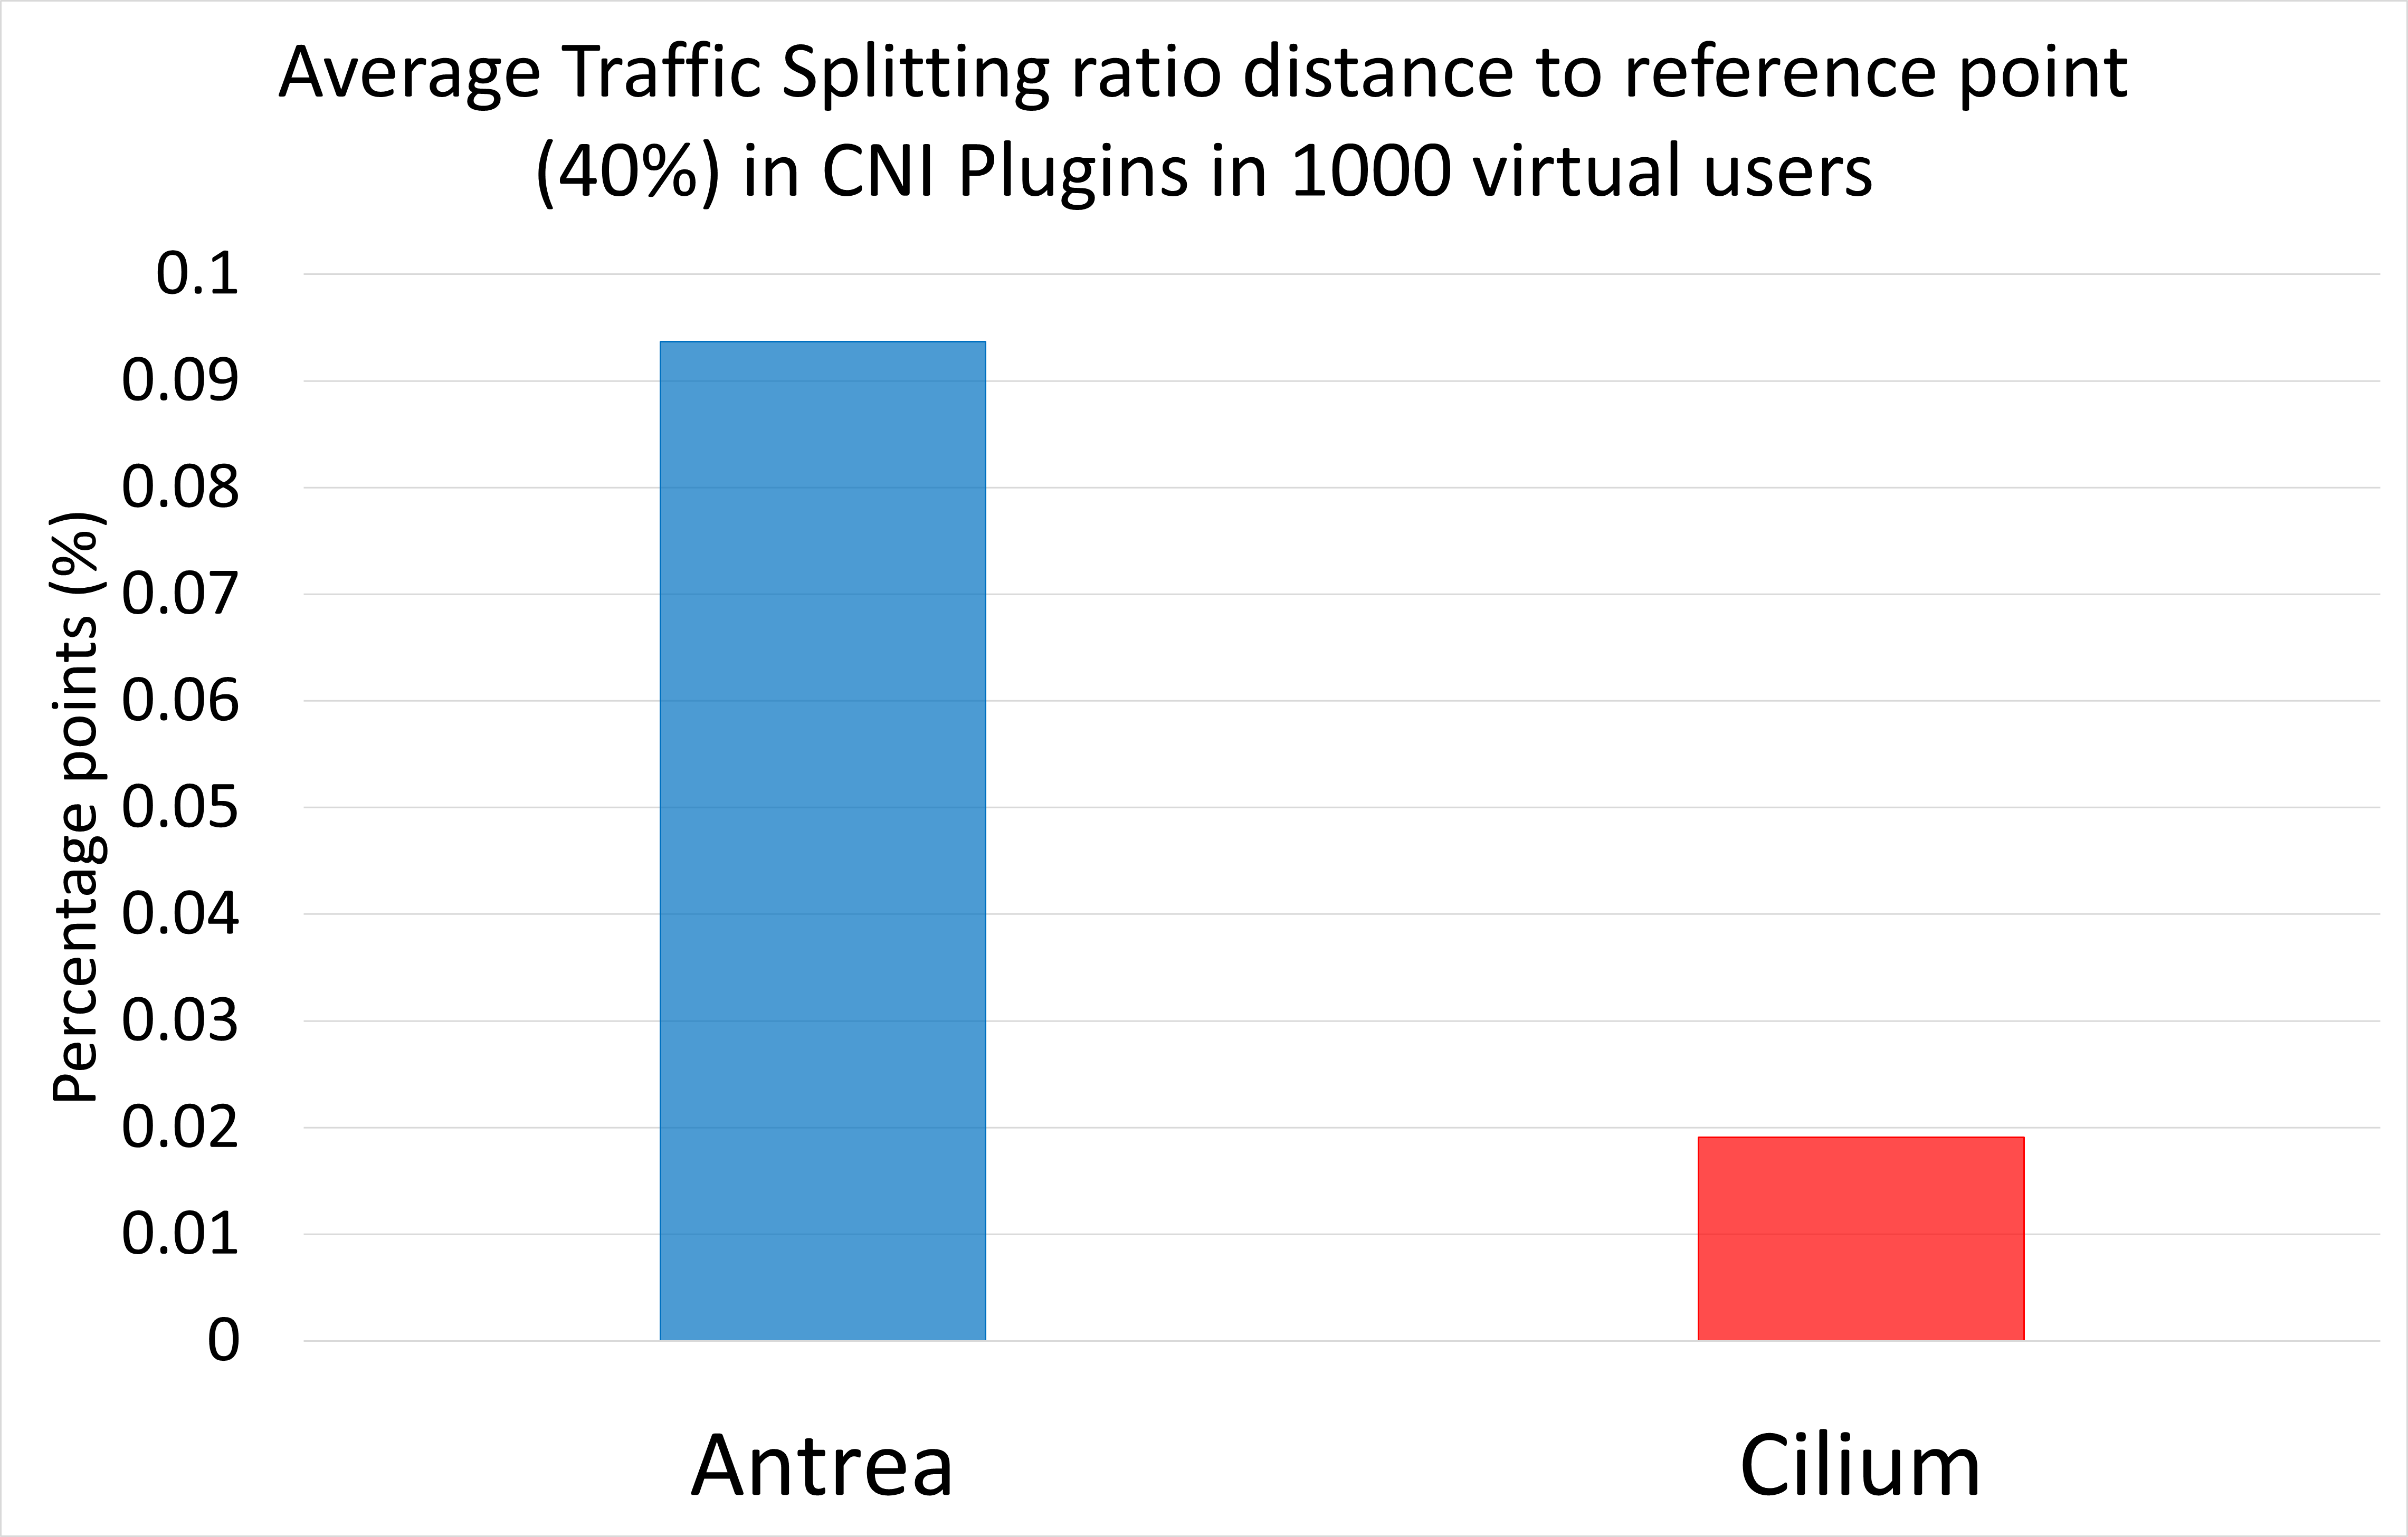
\includegraphics[width=\textwidth]{plots/traffic-splitting/time_window_5_1000vu_reference_cloud.png}
        \label{fig:reference_1000vu}
        \caption{}
    \end{subfigure}

    \caption{Average traffic splitting ratio distance to reference point in increasing virtual users, (a) one, (b) ten, (c) hundred, (d) thousand }
    \label{fig:referencesIngress}
\end{figure}

Analyzing plots in figure~\ref{fig:avg_vus} show overlapping confidence intervals in all cases, indicating some variability in the results. However, when averaging the values, it becomes clear that cilium performs better, especially as the number of VUs is one or a thousand. The distance to reference points can be seen in figure~\ref{fig:referencesIngress}. The overlapping confidence intervals show statistical uncertainty, but the average values demonstrate that cilium performs higher accuracy traffic weighting compared to Antrea and nginx test case.
